% !TEX program = pdflatex
% !TEX encoding = UTF-8 Unicode
 
% Plantilla, basada en la clase `scrbook` del paquete KOMA-script,  para la elaboración de un TFG siguiendo las directrices del la comisión del Grado en Matemáticas de la Universidad de Granada.

% Francisco Torralbo Torralbo

\documentclass[print, color]{ugrTFG}

% VERSIÓN ELECTRÓNICA PARA TABLETA
% Cambiando la opción "print" por "tablet" generaremos un pdf adaptado para leerlo en tabletas de 9 pulgadas.




\usepackage[]{graphicx}
\usepackage{eurosym}
\usepackage[]{wrapfig}
\usepackage[]{subcaption}
\usepackage{color}   %May be necessary if you want to color links
\usepackage[spanish,es-tabla]{babel}
\usepackage{hyperref}
\usepackage[a4paper , bindingoffset=0.2in, right=1in, left=1.4in,
            top=2in, bottom=2in, footskip=.3in]{geometry}
\usepackage[skip=10pt plus1pt, indent=40pt]{parskip}
\usepackage{indentfirst}
\usepackage{tabto}     
\usepackage{amsmath}
\usepackage{amsthm}
\usepackage{amssymb}
\usepackage[titletoc,toc,page]{appendix}
\definecolor{backcolour}{rgb}{0.95,0.95,0.92}
\usepackage{listings}
\usepackage{amsfonts}
\usepackage{mathabx}
\usepackage{verbatim}
\usepackage{longtable}

\usepackage{pdfpages}
\usepackage{soul}
\usepackage[strict]{changepage}
\usepackage[figurename=Figura]{caption}
\usepackage{afterpage}
\usepackage{lipsum}
\usepackage{fancyhdr}
\usepackage{hyperref}
\usepackage{float} % para [H]
\usepackage{enumitem}

\renewcommand{\appendixtocname}{Ap\'endices}
\renewcommand{\appendixpagename}{Ap\'endices}

\newcommand{\highlight}[1]{%
  \colorbox{yellow}{\parbox{\dimexpr\linewidth-2\fboxsep\relax}{\strut #1}}%
}


\newcommand{\ttimes}{{\,\otimes\,}}
\newcommand{\gtimes}{{\,\otimes_g\,}}
\newcommand{\bx}{\textnormal{\textbf{x}}}
\newcommand{\by}{\textnormal{\textbf{y}}}
\newcommand{\ba}{\textnormal{\textbf{a}}}
\newcommand{\bb}{\textnormal{\textbf{b}}}
\newcommand{\bu}{\textnormal{\textbf{u}}}
\newcommand{\bv}{\textnormal{\textbf{v}}}
\newcommand{\bw}{\textnormal{\textbf{w}}}
\newcommand{\kroprod}{\textnormal{\bigodot}}
\setlength{\parindent}{0pt}




% -------------------------------------------------------------------
% INFORMACIÓN DEL TFG Y EL AUTOR
% -------------------------------------------------------------------

\newcommand{\miTitulo}{Mejora de la Interpretabilidad en Modelos de Clasificación de Lesiones Cancerosas en Biopsias de Próstata mediante Técnicas de XAI.\xspace}
\newcommand{\miNombre}{Carlos Lara Casanova\xspace}
\newcommand{\miGrado}{Máster en Ciencia de Datos e Ingeniería de Computadores}
\newcommand{\miFacultad}{ETS Ingeniería Informática y de Telecomunicación}
\newcommand{\miUniversidad}{Universidad de Granada}

% Añadir tantos tutores como sea necesario separando cada uno de ellos mediante el comando `\medskip` y una línea en blanco
\newcommand{\miTutor}{
  Francisco Herrera Triguero\\ \emph{Departamento de Ciencias de la Computación e Inteligencia Artificial} 

  % Añadir tantos tutores como sea necesario. 

  \medskip
  Iván Sevillano-García \\ \emph{Departamento de Ciencias de la Computación e Inteligencia Artificial}
  }

\newcommand{\miCurso}{2024-2025\xspace}


\hypersetup{
	pdftitle={\miTitulo},
	pdfauthor={\textcopyright\ \miNombre, \miFacultad, \miUniversidad}
}

\begin{document}

\maketitle

% -------------------------------------------------------------------
% FRONTMATTER
% -------------------------------------------------------------------
\frontmatter % Desactiva la numeración de capítulos y usa numeración romana para las páginas

% !TeX root = ../tfg.tex
% !TeX encoding = utf8
%
%*******************************************************
% Declaración de originalidad
%*******************************************************

\thispagestyle{empty}

\hfill\vfill

\textsc{Declaración de originalidad}\\\bigskip

D./Dña. \miNombre \\\medskip

Declaro explícitamente que el trabajo presentado como Trabajo de Fin de Máster (TFM), correspondiente al curso académico \miCurso, es original, entendido esto en el sentido de que no he utilizado para la elaboración del trabajo fuentes sin citarlas debidamente.
\medskip

En Granada a \today 
\vspace{3cm}
\begin{center} 
Fdo: \miNombre 

\end{center}

\vfill

\cleardoublepage
\endinput
   
% !TeX root = ../tfg.tex
% !TeX encoding = utf8

%*******************************************************
% Table of Contents
%*******************************************************
\phantomsection
\pdfbookmark[0]{\contentsname}{toc}

\setcounter{tocdepth}{2} % <-- 2 includes up to subsections in the ToC
\setcounter{secnumdepth}{3} % <-- 3 numbers up to subsubsections

\tableofcontents 

%*******************************************************
% List of Figures and of the Tables
%*******************************************************

    % *******************************************************
    %  List of Figures
    % *******************************************************    
    \phantomsection 
    % \listoffigures

    %*******************************************************
    % List of Tables
    %*******************************************************
    \phantomsection 
    % \listoftables
    
    %*******************************************************
    % List of Listings
    % The package \usepackage{listings} is needed
    %*******************************************************      
	  % \phantomsection 
    % \renewcommand{\lstlistlistingname}{Listados de código}
    % \lstlistoflistings 

\cleardoublepage
            
% !TeX root = ../tfg.tex
% !TeX encoding = utf8

%*******************************************************
% Agradecimientos
%*******************************************************

\chapter{Agradecimientos}

Gracias a Francisco e Iván por brindarme la oportunidad de trabajar con ellos y guiarme durante la realización de este trabajo. Gracias a mi familia por apoyarme durante el tiempo que me llevó desarrollar este trabajo. 
\cleardoublepage
\endinput
            % Opcional

% !TeX root = ../tfg.tex
% !TeX encoding = utf8
%
%*******************************************************
% Summary
%*******************************************************

\selectlanguage{english}
\chapter{Summary}
\paragraph*{KEYWORDS:} neural networks, xai, explainable ai, prediction, explainability, artifical inteligence, machine learning, computer vision, deep learning, prostate cancer, gleason score, gleason groups.  

Aquí va el resumen en inglés
\thispagestyle{empty}


\selectlanguage{spanish} 
\endinput
                    
% !TeX root = ../tfg.tex
% !TeX encoding = utf8
%
%*******************************************************
% Introducción
%*******************************************************

% \manualmark
% \markboth{\textsc{Introducción}}{\textsc{Introducción}} 

\chapter{Resumen}

\paragraph*{PALABRAS CLAVE:} redes neuronales, xai, ia explicable, clasificación, explicabilidad, inteligencia artificial, aprendizaje automático, visión por computador, aprendizaje profundo, cáncer de próstata, gleason score, gleason groups.

Resumen en español.
\thispagestyle{empty}

\endinput
               

% -------------------------------------------------------------------
% MAINMATTER
% -------------------------------------------------------------------
\mainmatter % activa la numeración de capítulos, resetea la numeración de las páginas y usa números arábigos

\newpage
\chapter{Introducción}

En 2020, el \textbf{cáncer de próstata}, (\textit{Prostate Cancer, PCa}) fue el segundo tipo de cáncer más frecuente, y el quinto más mortal, en varones \cite{GlobalCancer}. Una \textbf{biopsia de próstata} es una prueba que consiste en la extracción de pequeños tejidos de la próstata para examinar posibles signos de cáncer (Ver Figura \ref{fig:biopsias_ejemplos}). El \textbf{Sistema de Puntuación de Gleason} (\textit{Gleason Score}) es una calificación, en el rango de 2 a 10, que se da a biopsias de la próstata tras ser examinadas bajo un microscopio \cite{GleasonGov}. Valores más altos indican cánceres más agresivos y de crecimiento más rápido. En 2014 la \textbf{Sociedad Internacional de Patología Urológica} (\textit{International Society of Urological Pathology, ISUP}) propuso un nuevo sistema basado en la Puntuación de Gleason, que propone cinco grupos ordenados (\textbf{Gleason Groups, GGs}) \cite{ISUP2014Disc}:
\begin{itemize}
\item \textbf{GG1: } Cáncer de grado bajo. Puntuación de gleason 6 o inferior.
\item \textbf{GG2: } Cáncer de grado medio. Puntuación de gleason 7.
\item \textbf{GG3: } Cáncer de grado medio pero más agresivo que GG2. Puntuación de gleason 7 pero percibido más agresivo.
\item \textbf{GG4: } Cáncer de grado alto. Puntuación de gleason 8.
\item \textbf{GG5: } Cáncer de grado alto. Puntuación de gleason 9 o 10.
\end{itemize}

\begin{figure}[H]
    \centering
    \begin{subfigure}[b]{0.3\textwidth}
        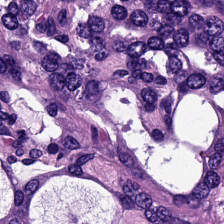
\includegraphics[width=\linewidth]{images/EjemploBiopsia1.png}
    \end{subfigure}
    \hfill
    \begin{subfigure}[b]{0.3\textwidth}
        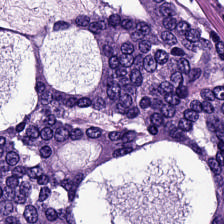
\includegraphics[width=\linewidth]{images/EjemploBiopsia2.png}
    \end{subfigure}    
    \hfill
    \begin{subfigure}[b]{0.3\textwidth}
        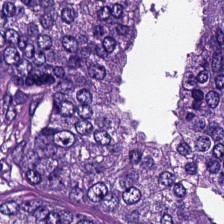
\includegraphics[width=\linewidth]{images/EjemploBiopsia3.png}
    \end{subfigure}

    \caption{Tres imágenes correspondientes a tres biopsias distintas.}
    \label{fig:biopsias_ejemplos}
\end{figure}


En el campo de la \textbf{Inteligencia Artificial (IA)}, la necesidad de asegurar transparencia y confiabilidad a dado pie a acuñar el término de \textbf{Inteligencia Artificial eXplicable} (\textit{eXplainable Artificial Inteligence, XAI}) \cite{XAIManifesto}. El uso de XAI es especiamente importantes en ámbitos donde la toma de decisiones repercute directamente en la vida de las personas, como es el caso de la medicina. La Unión Europea ha propuesto una \href{https://eur-lex.europa.eu/eli/reg/2024/1689/oj}{regulación} para el uso de IA asistida en estos aspectos, entre ellos, que estos sistemas sean capaces de explicar sus decisiones de forma clara y comprensible.

Dentro del campo de la XAI, hay diferentes propuestas para la evaluación y la mejora de las explicaciones generadas. Por un lado, herramientas como \textbf{REVEL} \cite{REVEL} permiten analizar la calidad de las mismas de manera robusta. Por otro, enfoques como \textbf{X-SHIELD} \cite{XSHIELD} buscan mejorar las explicaciones mediante técnicas de regularización que aseguran el buen comportamiento de la generación de explicaciones. Aplicar estas técnicas en imagen médica puede ayudar a mejorar la interpretación de las personas profesionales de la salud de las decisiones de una IA que asista.

En este contexto este Trabajo de Fin de Máster trata de resolver el problema de \textbf{construir un modelo de IA de clasificación para lesiones cancerosas en biposias de próstata} y de la \textbf{mejora en interpretabilidad del modelo mediante técnicas de XAI}. Para esto se vamos a utilizar las herramientas REVEL y XSHIELD, y propondremos posibles mejoras de XSHIELD.


El TFM se estructura del siguiente modo. En primer lugar vamos a introducir los fundamentos teóricos necesarios para el correcto entendimiento del trabajo realizado (Capítulo \ref{cap:ft}). Después se va a hacer un estudio del estado del arte (Capítulo \ref{cap:eda}). A continuación presentamos las propuestas de este TFM (Capítulo \ref{cap:met}). En el Capítulo \ref{cap:exp} se describe el conjunto de datos con el que trabajamos, los distintos experimentos que realizamos y discutimos los resultados . Finalmente en el Capítulo \ref{cap:conc} se incluyen conclusiones y posibles trabajos futuros.


\section{Objetivos}

El objetivo principal del TFM es la utilización (y propuesta) de técnicas de evaluación y mejora de explicaciones  para modelos de clasificación de imágenes para detección de tejidos cancerosos en biopsias de próstata. Para el desarrollo del TFM, se divide el objetivo en distintos subobjetivos:

\begin{itemize}
\item Revisión del estado del arte.
\item Estudio del código que implementa \cite{REVEL, XSHIELD} para su correcto entendimiento.
\item Proposición de nuevos métodos XAI para mejora de explicaciones para modelos de explicación.
\item Modificación del código para implementar dichas propuestas.
\item Diseño de los experimentos a realizar e implementación de estos.
\item Evaluación de los resultados y subsecuente discusión.
\end{itemize}

Aquí introduciría el objetivo principal del TFM y lo dividiría en algunos sub-objetivos (revisión del estado del arte, estudio de las implementaciones de las métricas ReVEL/regularización X-Shield, proposición de mis regularizaciones, implementación de estas, experimentación y finalmente evaluación/discusión de estos). 


\section{Planificación}

\highlight{
En esta sección hablo de cómo me he planificado el proyecto según estudio del problema/diseño de mis modelos/implementación/experimentación (haría una tabla). Luego haría una comparación de mi planificación vs cómo se ha repartido finalmente y haría una estimación final de cuántas horas me ha llevado el TFM y en cuánto se estima el coste del proyecto final.

POR HACER
}


\clearpage
\chapter{Fundamentos teóricos} \label{cap:ft}


\section{Aprendizaje automático}

El \textbf{aprendizaje automático} (AA) o \textbf{machine learning} (ML) es una rama de la \textbf{inteligencia artificial} que se encarga del desarrollo de algoritmos que aprendan de datos o experiencias con el fin de mejorar su rendimiento en ciertas tareas \cite{alpaydin_introduction_2010-1, Mostafa2012, PatternRecogLibro, pml1Book}. Estos algoritmos disponen de un \textbf{modelo} definido por ciertos parámetros y dichos parámetros serán los que se aprendan a través del \textbf{entrenamiento} o \textbf{aprendizaje}.

Para saber a qué nos referimos cuando se habla de que el algoritmo \textit{``aprende''} conviene destacar la siguiente definición proveniente de \cite{mitchell_machine_1997}: \textit{``Un programa se dice que aprende de una experiencia E con respecto a una clase de tareas T y a una medida de rendimiento T, si su rendimiento en las tareas en T, medido por P, mejora con la experiencia E."}

El AA se utiliza habitualmente para resolver problemas complejos que no se pueden o se saben resolver con algoritmos tradicionales diseñados por humanos. Además se requiere tener datos de los que poder aprender. Algunos de los campos donde se utilizan el AA para resolver este tipo de problemas son el procesamiento de lenguaje natural, el reconocimiento del habla o la visión por computador, entre muchos otros.

Los algoritmos de AA se clasifican en distintos paradigmas dependiendo de los datos o experiencia de la que se disponga. Existen tres paradigmas principales: el \textbf{aprendizaje supervisado}, el \textbf{aprendizaje no supervisado} y el \textbf{aprendizaje por refuerzo} \cite{Mostafa2012,Goodfellow-et-al-2016}.

El aprendizaje supervisado hace referencia a los algoritmos de AA en los que se tiene un conjunto de datos agrupados en pares dato-\textbf{etiqueta}. La etiqueta se corresponde con la salida que se requiere del algoritmo de AA cuando tenga de entrada dicho dato. Un ejemplo típico de conjunto de datos de este tipo sería un conjunto de imágenes de números escritos a mano y para cada imagen el número que está escrito en dicha imagen.

El aprendizaje no supervisado hace referencia a los algoritmos de AA en los que se disponen de datos que no están etiquetados. En este tipo de algoritmos no se quiere aprender algo específico de los datos sino más bien encontrar patrones o estructurar los datos de entrada. Por ejemplo se dispone de distinta información relativa a libros (autor, título, número de páginas, etc) y el algoritmo categoriza los libros en distintas categorías, aunque no se sepa a qué se corresponde cada categoría.

En el aprendizaje por refuerzo no se disponen de datos de entrada, sino de una entrada y una \textit{recompensa} correspondiente a cada salida posible para dicha entrada. Este tipo de AA es especialmente útil para aprendizaje de juegos o tareas relacionadas con la teoría de control.

Para este TFG es relevante el aprendizaje supervisado. En particular serán relevantes los dos siguientes problemas típicos de aprendizaje supervisado.

\subsection{Problema de clasificación}
Este problema trata de clasificar las entradas de un tipo concreto en un número de clases $k$. Es decir, para una entrada el programa deberá clasificar dicha entrada en una de las $k$ clases. Por lo tanto el algoritmo produce una función $f:\mathbb{R}^n \rightarrow \{1,...,k\}$ que a cada entrada $\bx$ le asocie una clase $y = f(\bx)$. Dicha función tratará de aproximar una función objetivo $g$ que clasifique perfectamente todas las entradas.

Para este problema se disponen de una serie de datos de entrada $\{\bx_1,...,\bx_N\}$ con $\bx_i\in\mathbb{R}^n$ y sus clases correspondientes $\{y_1,...,y_N\}$ con $y_i \in \{1,...,k\}$. 

Algunas formas de resolver estos problemas son mediante árboles de clasificación, máquinas de vectores-soporte o mediante redes neuronales.

Un caso particular de este problema que es más relevante para este trabajo es el caso en el que hay dos clases. Este problema se denomina \textbf{problema de clasificación binaria}. En este TFG se tratará de determinar visibilidad de puntos de la cara de una persona en una imagen luego las dos clases se corresponden con visible o no visible.

\subsection{Problema de regresión}
Este problema es similar al de clasificación, pero la función que aprende el algoritmo es de la forma $f:\mathbb{R}^n \rightarrow\mathbb{R}^m$. Por lo tanto ahora el programa debe predecir un valor numérico (o varios si $m > 1$) para una entrada concreta. Al igual que ocurría en el problema de clasificación se disponen de una serie de datos de entrada y el resultado que se espera del programa para dichas entradas, es decir $\{\bx_1,...,\bx_N\}$ con $\bx_i\in\mathbb{R}^n$ y  $\{\by_1,...,\by_N\}$ con $\by_i \in \mathbb{R}^m$. 

Algunas formas de resolver este tipo de problemas son mediante la regresión lineal, máquinas de vectores-soporte o redes neuronales.

\subsection{Optimización} \label{optimización}

Ya se ha hablado de algunos problemas de AA. En ellos se quiere mejorar el rendimiento de una función $f$ para una tarea. La forma en la que se mide el rendimiento es mediante otra función denominada \textbf{función de error}, \textbf{función de pérdida} o \textbf{función de coste} \cite{Goodfellow-et-al-2016}. Esta función mide el error de la aproximación de la salida de $f$ para una entrada $\bx$. Por lo tanto se busca minimizar dicha función.

Por ejemplo, una función de coste habitual es el error cuadrático medio:

\begin{align*}
ECM = \frac{1}{n}\sum_{i=1}^{n}(y_i-\hat{y_i})^2
\end{align*} 

Donde $\hat{y_i}$ es la predicción de nuestro modelo para un dato $x_i$ y $y_i$ es el valor correcto de salida para esa entrada.

El método principal en el AA para minimizar dicha función es el \textbf{gradiente descendente}. Este método iterativo se basa en que, para una función multivariable dos veces diferenciable, el gradiente de dicha función en ese punto (que es un vector) apunta en la dirección contraria al ascenso más empinado. Por lo tanto tomando pasos en la dirección contraria al gradiente, debería disminuir la función de coste y por lo tanto dar un mejor rendimiento.


Se recuerda que el gradiente de una función $E:\mathbb{R}^n \rightarrow \mathbb{R}$ en un punto no es más que le vector compuesto de las derivadas parciales respecto a cada variable en dicho punto:

\begin{align*}
\nabla E(\bw) = \left[ \frac{\partial E}{\partial x_1}(\bw),...,\frac{\partial E}{\partial x_n}(\bw) \right]^\top
\end{align*}


Normalmente, el método utilizado para resolver el problema de AA hace que las funciones que se pueden representar en la solución estén parametrizadas por un vector de parámetros o \textbf{pesos} $\bw$. Por ejemplo, en un problema de regresión con función objetivo $f:\mathbb{R}^n \rightarrow \mathbb{R}$ que se plantea resolver mediante regresión lineal se tiene que la función que se aprende toma la forma: 
\begin{align*}
f_\bw(\bx) = \bw^\top \bx \quad \quad , \bx \in \mathbb{R}^n, \bw \in \mathbb{R}^n
\end{align*}
 
Donde el vector $\bw$ son los parámetros que se pueden cambiar a la función para mejorar su rendimiento.

La función de coste dependerá de dichos parámetros. Luego el gradiente descendiente cambiará el valor de los parámetros en cada paso buscando minimizar la función de coste. Estos cambiarán según la siguiente regla:
\begin{align*}
\bw_n = \bw - \eta \nabla E(\bw)
\end{align*} 
Donde $\bw_n\in\mathbb{R}^l$ son los nuevos parámetros, $\bw\in\mathbb{R}^l$ son los parámetros del paso actual, $E$ es el función de coste, $\nabla E$ representa el gradiente de $E$ y $\eta$ es un hiperparámetro (parámetro del algoritmo) en $\mathbb{R}$ llamado \textbf{learning rate}(lr).

El lr determina el tamaño de los pasos tomados por el algoritmo en cada iteración. Un valor del lr alto puede hacer que	el algoritmo converja más rápido pero también puede hacer que el algoritmo no llegue a converger o se salte soluciones. Por otro lado un valor bajo del lr hace que el algoritmo converja demasiado lento a un mínimo de la función. En la práctica se suelen utilizar métodos que hacen que el lr varíe a lo largo del entrenamiento, normalmente de mayor a menor.

El algoritmo del gradiente descendente inicia los pesos $\bw$ a un valor aleatorio y empieza a iterar con la regla anteriormente descrita buscando reducir el error en cada paso durante un número de \textbf{épocas} (cada época itera sobre todos los datos de entrenamiento), aunque hay otros criterios de parada del algoritmo. En caso de ser satisfactorio el algoritmo para en un mínimo local (o global idealmente) del error de pérdida. 

El cálculo del gradiente del error conlleva utilizar todos los datos de entrenamiento lo que en la práctica resulta muy costoso. Por ello se suele utilizar el \textbf{descenso de gradiente estocástico} (SGD), que en cada paso calcula una estimación del gradiente real a partir de un subconjunto aleatorio de los datos de entrenamiento denominado \textbf{minibatch}. Destacar que los datos de entrenamiento no se deben repetir entre \textit{minibatches} hasta que se hayan utilizado todos los de entrenamiento entre cada repetición.

\subsection*{Sobreentrenamiento}

Cuando se optimiza un modelo, puede ocurrir que el modelo se ajuste muy bien para los datos de entrada con los que se ha entrenado, pero tenga mal rendimiento para datos con los que no se ha entrenado y por lo tanto no generaliza bien lo aprendido de los datos de entrenamiento al problema. Cuando esto ocurre se dice que el modelo se ha \textbf{sobreentrenado} o \textbf{sobreajustado}. Una forma de identificar este problema es guardándonos un número de datos con los que no se va a entrenar el modelo y comparar el error del modelo a lo largo del entrenamiento de los datos de entrenamiento con los que nos se han guardado. El sobreentrenamiento se puede observar cuando el error en los datos con los que no se entrena empieza a aumentar a medida que se sigue entrenando el modelo como se puede ver en la Figura \ref{fig:sobreentrenamiento}.


\begin{figure}[h]
\noindent
\makebox[\textwidth]{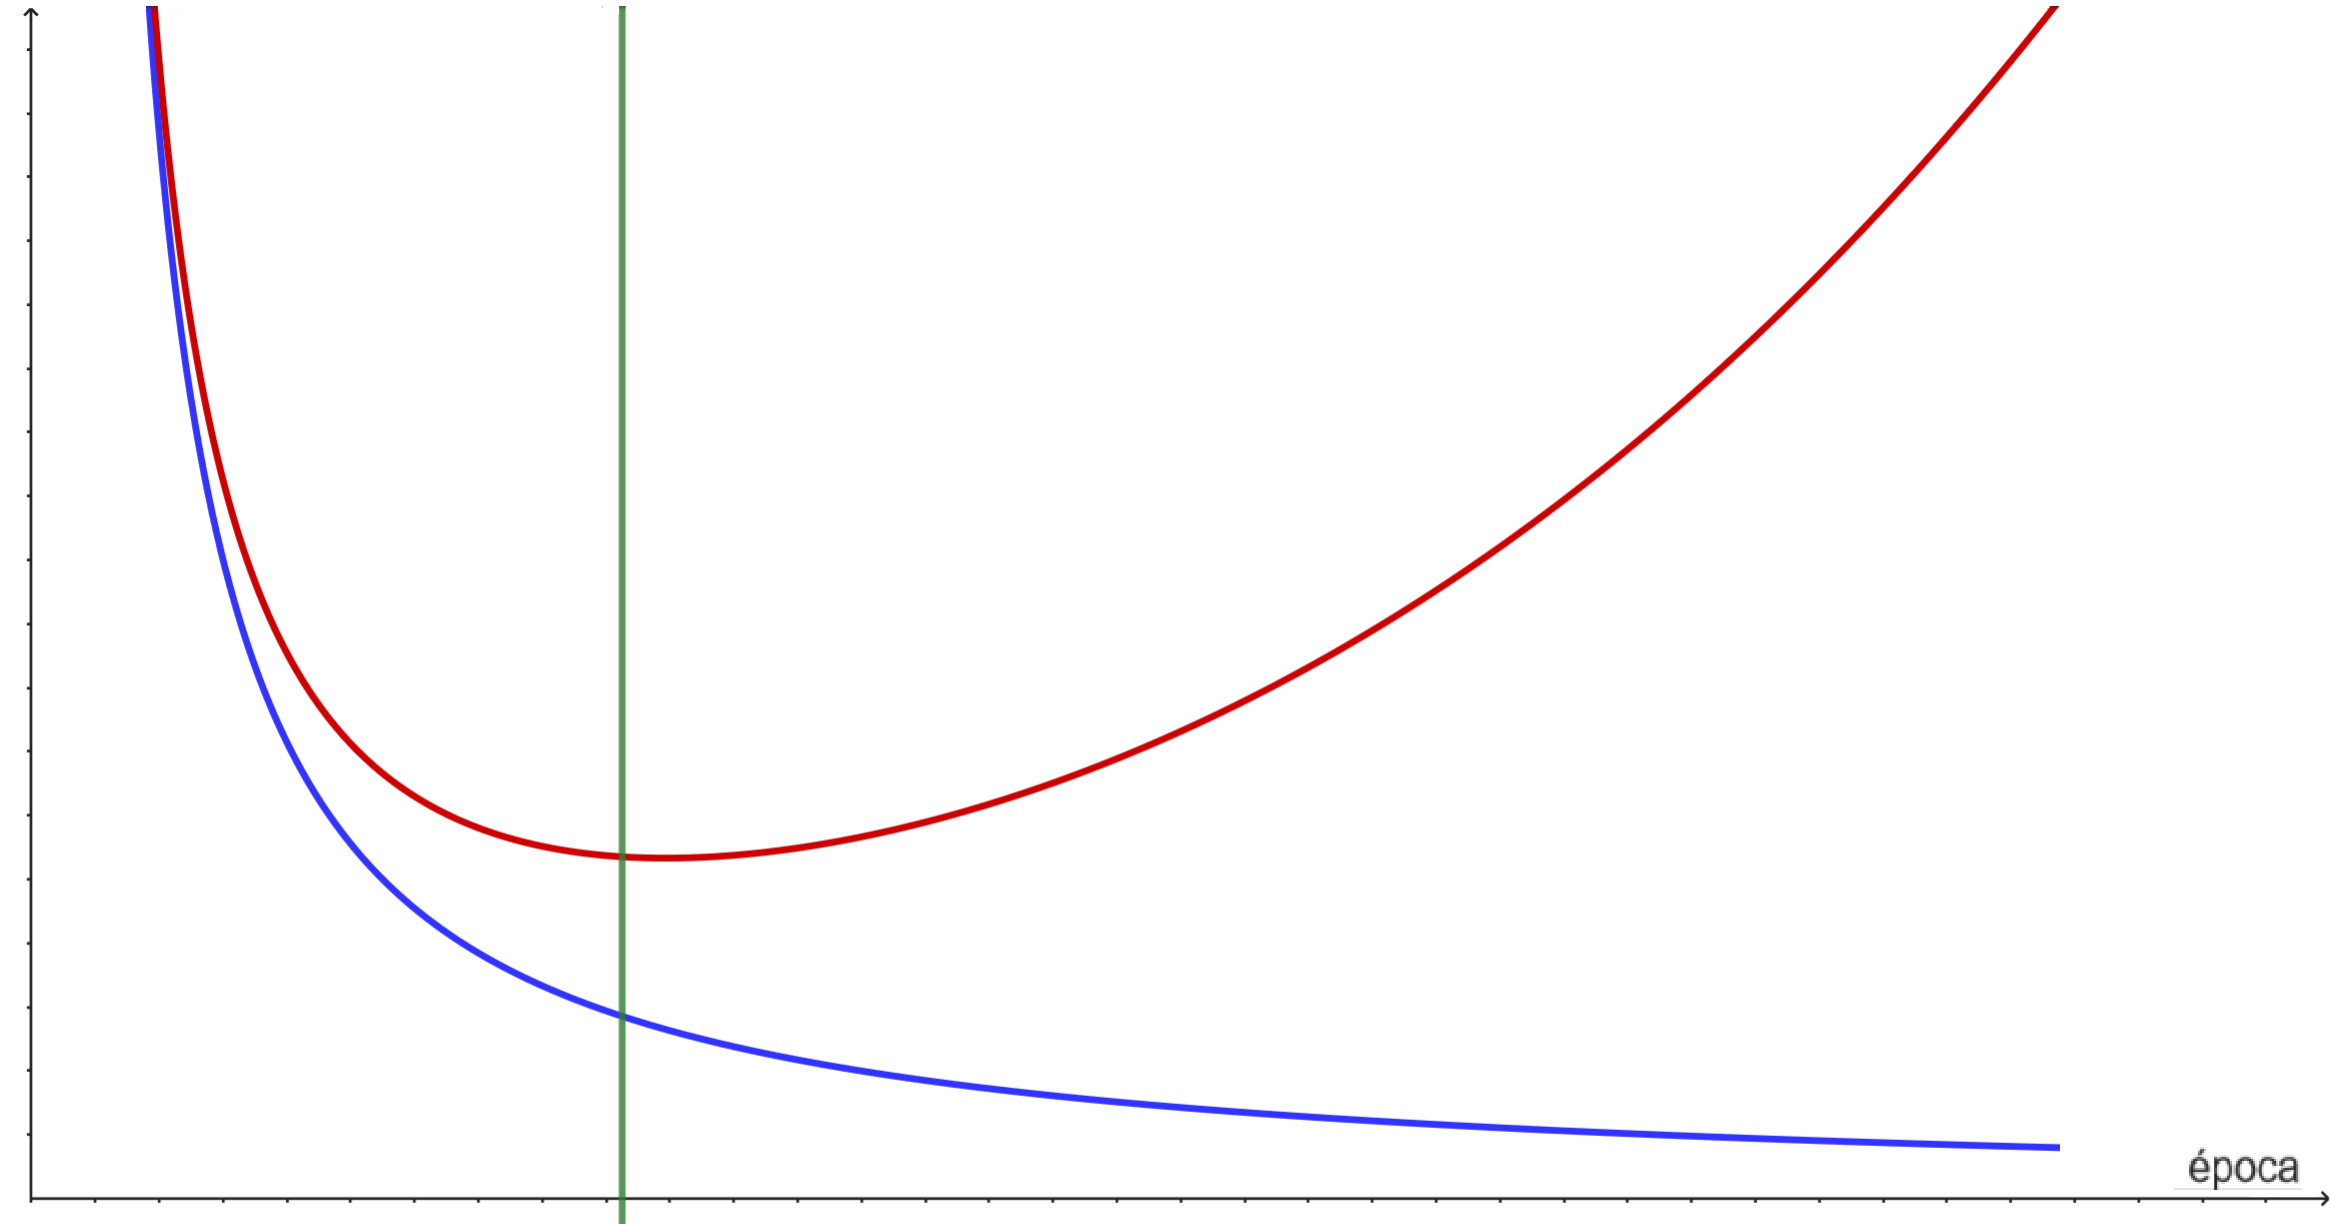
\includegraphics[scale=0.3]{images/sobreentrenamiento}}
\caption{ Esta figura muestra el error en entrenamiento en azul y el error en los datos con los que no se entrena el modelo en rojo a lo largo del entrenamiento. Se puede ver como a partir de la línea verde el modelo sigue aprendiendo de los datos de entrada pero empeora el poder de generalización con los datos con los que no entrena.}
\label{fig:sobreentrenamiento}
\end{figure}

\section{Deep Learning}
\textbf{Deep learning}(DL) \cite{DeepLearningFoundationsConcepts, Goodfellow-et-al-2016, LeCun-Yann-Bengio, UnderstandingDeepLearning, Schmidhuber_2015} es un subcampo del AA determinado por los métodos con los que aprende y tipo de datos con los que trata. Los algoritmos de DL pueden tratar datos poco estructurados como pueden ser imágenes o textos. Este tipo de algoritmos automatizan la extracción de características, es decir, determinan qué información de los datos es relevante para la resolución del problema. Esto elimina mucha de la intervención necesaria por los humanos a la hora de crear el algoritmo.

El DL en los últimos años ha supuesto un avance significativo en muchos campos en los que apenas se avanzaba con otras técnicas de IA como el reconocimiento del habla o el procesamiento de lenguaje natural.

\subsection*{Redes neuronales}
Una \textbf{red neuronal} (\textit{artificial neural network}, ANN) \cite{NNPatternRecogLibro,Haykin,NNTricks} es un modelo de AA que consiste en una red conectada de \textbf{nodos} o \textbf{neuronas}. Cada neurona recibe una serie de números reales (señales) de las neuronas conectadas a esta, hace una operación con dichos números que resulta en otro número real y lo manda a los nodos conectados a esta. 

La operación que realiza una neurona con $n\in\mathbb{N}$ entradas es la siguiente:

\begin{align} \label{eq:salida_neurona}
y = \sum_{i=1}^{n}\sigma({w_i x_i} + w_0) \quad \quad , w_i,x_i \in \mathbb{R}
\end{align}

Dónde $x_i$ son las entradas de la neurona, $w_i$ son los \textbf{pesos} de la neurona, en particular a $w_0$ se le denomina sesgo, y $\sigma$ es una función de los números reales a los números reales y se le denomina \textbf{función de activación} \cite{article_func_activacion}. Al conjunto de los pesos de todas las neuronas de una red se les denomina, naturalmente, \textbf{pesos de la red}. A través de la modificación de dichos pesos es como se entrenará a una red para realizar una tarea concreta.

Existen dos tipos de ANN según el flujo de la información dentro de la red. Nos centramos en el caso en el que este flujo es una única dirección, en cuyo caso se tiene una \textbf{red neuronal hacia delante} (\textit{feedforward neural network} o \textit{multilayer perceptron}, MLP).

Las MLP son el modelo fundamental del \textit{Deep Learning}. Estas están compuestas por distintas \textbf{capas}, cada una compuesta de varias neuronas en paralelo. La primera capa es la \textbf{capa de entrada} que recibe la entrada a la red y la propaga a la siguiente capa. Luego puede haber una o más \textbf{capas ocultas}, donde cada una de estas están compuestas de neuronas que reciben las señales de la capas anterior y propagan su salida a las neuronas de la siguiente capa. Por último está la \textbf{capa de salida} que está compuesta por uno o varias neuronas cuya salida se considera la salida de la red. El número de capas ocultas determina la \textbf{profundidad} de la red. Se puede ver un ejemplo de un modelo de este tipo en la figura \ref{fig:red_neuronal_ff}.


\begin{figure}[h]
\noindent
\makebox[\textwidth]{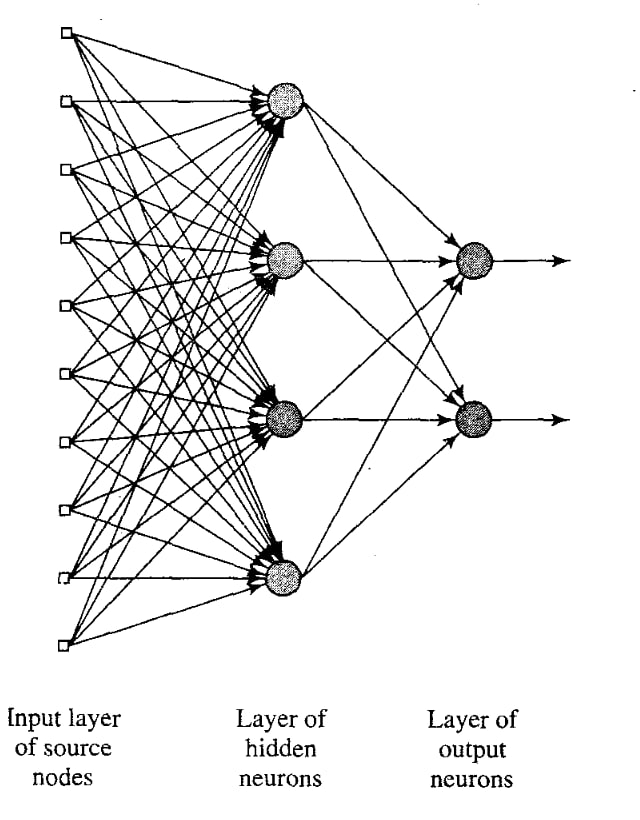
\includegraphics[scale=0.5]{images/MLP}}
\caption{ Ejemplo de ANN con una única capa oculta y con dos salidas. Imagen extraída de \cite{Haykin}.}
\label{fig:red_neuronal_ff}
\end{figure}

Si se considera ahora la función $f$ que implementa un red MLP, se tiene que esta depende de los pesos de la red. Una vez se tengan unos datos con los que entrenar la red y una función de coste que evalúe el rendimiento de la red, se puede aplicar el gradiente descendente estocástico para entrenar la red modificando los pesos de esta. Sin embargo, el cálculo del gradiente de la función de error en un red puede resultar muy costoso, especialmente para el cálculo de las derivadas parciales del error respecto de los pesos de las neuronas en las capas menos profundas. Es por esto que se suele utilizar un algoritmo, denominado \textbf{backpropagation}, para el cálculo del gradiente. 

Este algoritmo está basado en la aplicación de la regla de la cadena que dicta que si se tiene una función $f$ que depende de otra función $g$ que a su vez depende de otra función $h$, entonces se cumple que:
\begin{align*}
\frac{\partial f}{\partial z} = \frac{\partial f}{\partial g} \frac{\partial g}{\partial z}
\end{align*}

De esta forma se puede calcular la parcial de la función de coste respecto a los pesos de una capa utilizando las parciales respecto de los pesos de la siguiente. Luego aplicando esto desde el final al principio de la red, se consigue agilizar el cálculo del gradiente de la función de coste.

\subsection*{Funciones de activación}

Como se comenta en la ecuación \eqref{eq:salida_neurona}, la salida de una neurona es una suma ponderada de las entradas más un sesgo, a las que se le aplica una función de activación. La inclusión de este tipo de funciones es para evitar que la red sea lineal. Si la ecuación \eqref{eq:salida_neurona} fuese idéntica sin aplicar la función de activación entonces la salida de la red sería una función lineal respecto de la entrada, esto es, un polinomio de primer grado. Esto haría que la red no pudiera implementar funciones complejas lo que es necesario para aprender patrones más complejos presentes en los datos.  Es por esto que normalmente las funciones de activación deben ser funciones no lineales. Destacar que la función de activación debe ser derivable para poder calcular el gradiente de la función de coste con el algoritmo \textit{backpropagation} cuando se entrene la red.

Existen varias funciones de activación que se pueden utilizar, sin embargo son especialmente interesantes la función de activación \textbf{ReLU} (\textit{rectifier linear unit}) definida como $ f(x) = max\{0,x\}$ y la \textbf{sigmoidal} definida como $f(x) = \frac{1}{1+e^{-x}}$. Se pueden ver sus gráficas en la figura \ref{fig:ejemplos_activacion_relu} y la figura \ref{fig:ejemplos_activacion_sigmoidal}, respectivamente.

La función de activación ReLU es la que se suele usar en las neuronas de las capas ocultas pues contrarresta el \textbf{problema de desvanecimiento del gradiente}. Un problema que afecta al entrenamiento de las redes neuronales que causa que cuando se calcula el gradiente del error para actualizar los pesos este tome valores muy pequeños haciendo que los pesos de la red cambien muy lentamente. Esto dificulta, o incluso impide, el entrenamiento de la red. Además esta función de activación es la más usada normalmente y tiene mejor rendimiento en la mayoría de los casos.

La función de activación sigmoidal se suele utilizar en la capa de salida en los problemas de clasificación binarios.

\begin{figure}[h]
\noindent
\makebox[\textwidth]{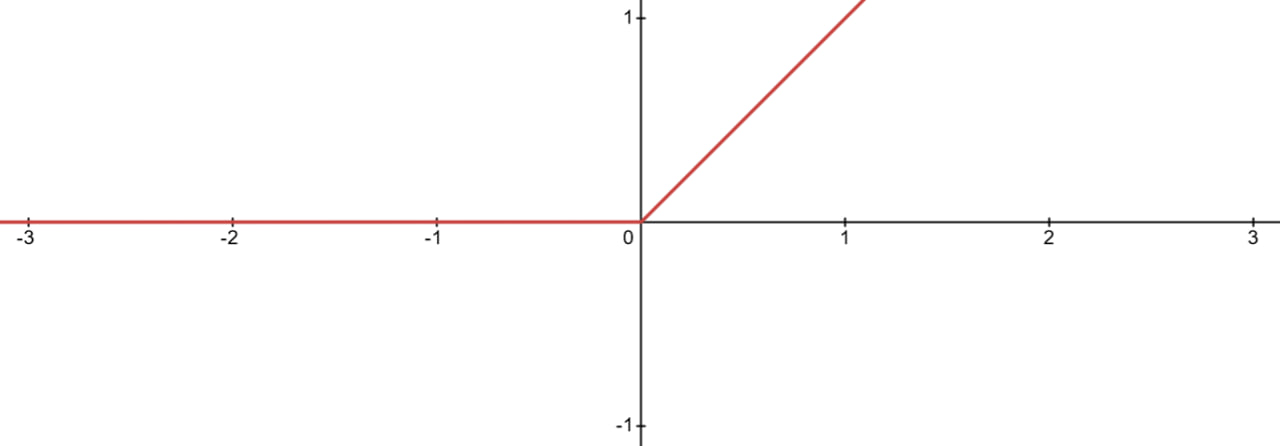
\includegraphics[scale=0.35]{images/relu}}
\caption{Función de activación ReLU.}
\label{fig:ejemplos_activacion_relu}
\end{figure}

\begin{figure}[h]
\noindent
\makebox[\textwidth]{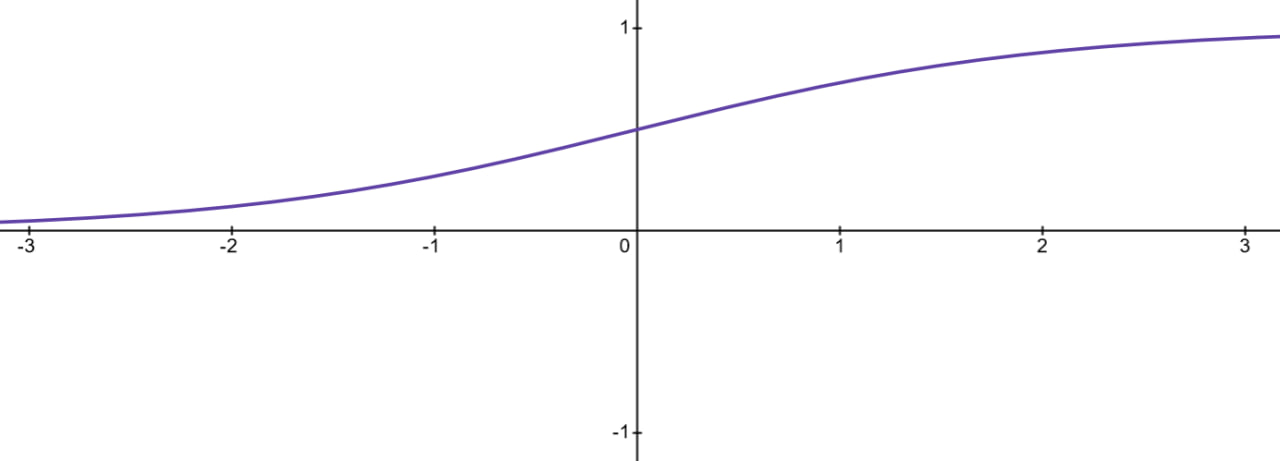
\includegraphics[scale=0.35]{images/sigmoidal}}
\caption{Función de activación sigmoidal.}
\label{fig:ejemplos_activacion_sigmoidal}
\end{figure}



\subsection*{Batch normalization}

\textbf{Batch normalization} \cite{ioffe2015batch} es una método consistente en normalizar los datos de entrada de cada capa. De esta manera se consigue independizar la distribución de los datos de entrada de cada capa de la red, con los parámetros aprendidos por la red. Está probado que este método hace que el entrenamiento de la red sea más estable y más rápido. Además también se sabe que tiene un efecto regularizador en la red, lo que disminuye la probabilidad de que la red sobreentrene.

\subsection*{Dropout}

\textbf{Dropout} \cite{hinton2012improving} se refiere a la técnica utilizada en redes neuronales consistente en ignorar algunas neuronas de forma aleatoria durante el periodo de entrenamiento. Usualmente se le da a cada neurona una probabilidad $p$ de ser ignorado, y en cada paso del algoritmo de entrenamiento se desconecta cada neurona de la red con dicha probabilidad. De esta forma se busca que ninguna neurona sea muy dependiente de la salida de otra neurona específica. Esta técnica regulariza la red lo que hace que la red sea menos propensa a sobreentrenar.

\subsection{Redes convolucionales}
La \textbf{redes convolucionales} (\textit{Convolutional neural networks}, CNN) \cite{9451544} son un tipo de red neuronal feedforward diseñadas para procesar datos en forma de múltiples arrays. En nuestro caso nos centraremos en el caso en el que la entrada son imágenes, que son arrays en 2 dimensiones (matrices) que contienen tres \textbf{canales}, uno por cada color.  La estructura las CNNs es una capa de entrada, seguida de varias capas ocultas y una capa de salida. Las capas ocultas suelen estar compuestas por una o varias \textbf{capas convolucionales} seguidas de una \textbf{capa de pooling}, esto repetido varias veces. Además al final de la red se suelen colocar una o varias \textbf{capas totalmente conectadas} hasta la capa de salida.

\subsection*{Capas convolucionales}
Una \textbf{convolución} es un operador matemático que recibe dos funciones $f,g:\mathbb{R}\rightarrow \mathbb{R}$ y la transforma en otra función $f\ast g$ definida como sigue:
\begin{align*}
(f \ast g)(t) = \int_{-\infty}^{\infty} f(x)g(t-x)dx
\end{align*}
Basado en este operador, existe la \textbf{convolución discreta} en 2 dimensiones, que se define como sigue:

\begin{align*}
(f\star g)[i,j] = \sum_{m=-\infty}^{\infty}\sum_{n=-\infty}^{\infty}f(m,n)g(i-m,j-n)
\end{align*}

Este operador no es más que la adaptación de la convolución al caso en el que $f$ y $g$ sean funciones discretas, es decir, definidas sobre los números enteros, $\mathbb{Z}$. Este es el operador que aplican las capas convolucionales a sus entradas. En el caso de las convoluciones aplicadas en una CNN $f$ se corresponde con la entrada de la capa convolucional y $g$ con el \textbf{núcleo}, \textbf{kernel} o \textbf{filtro}. de la convolución. El \textit{kernel} no es más que una matriz de dimensiones $n\times m$ de valores reales. Véase la Figura \ref{fig:ejemplo_convolucion} para ver un ejemplo de una convolución.

 
\begin{figure}[h]
\noindent
\makebox[\textwidth]{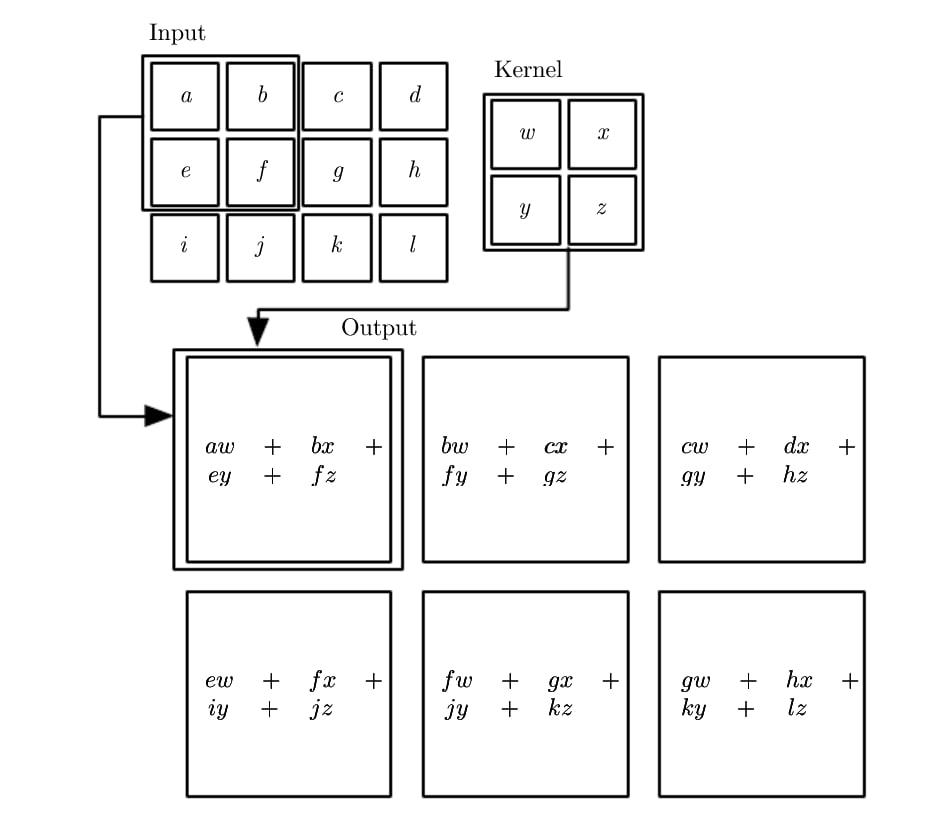
\includegraphics[scale=0.5]{images/ejemplo_convolucion}}
\caption{En esta imagen se puede ver un ejemplo de una convolución aplicada a una entrada de dimensiones $3\times 4$ por un kernel de dimensiones $2\times 2$. Se puede ver que la salida tiene tamaño $2\times 3$. Notablemente se puede ver que al contrario que en la definición de la operación de convolución dada, aquí no se le da la vuelta al kernel, como suele ocurrir en la práctica. Imagen extraída de \cite{Goodfellow-et-al-2016}.}
\label{fig:ejemplo_convolucion}
\end{figure}

Usualmente la entrada de las capas convolucionales tienen más de un canal (por ejemplo la capa inicial suele tener 3 canales, uno por cada color primario), en tal caso, el \textit{kernel} tiene tantos canales como la entrada y aplica cada uno a su canal correspondiente, sumando la salida. Para un ejemplo ver la Figura \ref{fig:ejemplo_convolucion_3canales}. A la salida de una convolución se le llama \textbf{mapa de características}. 

Por lo visto hasta ahora, el filtro se aplica posición a posición de izquierda a derecha y de arriba hacia abajo. Se denomina \textbf{stride} al parámetro que determina cada cuantas posiciones se aplica el filtro. Por ejemplo un stride de 1 aplica el filtro de forma normal. Otro parámetro que se utiliza es el \textbf{padding} que indica si se debe expandir la imagen por los bordes y con qué valores expandirla en caso de hacerlo. Por ejemplo, en la figura \ref{fig:ejemplo_convolucion} no se utiliza \textit{padding} y por lo tanto la salida tiene una fila y una columna menos.

\begin{figure}[h]
\noindent
\makebox[\textwidth]{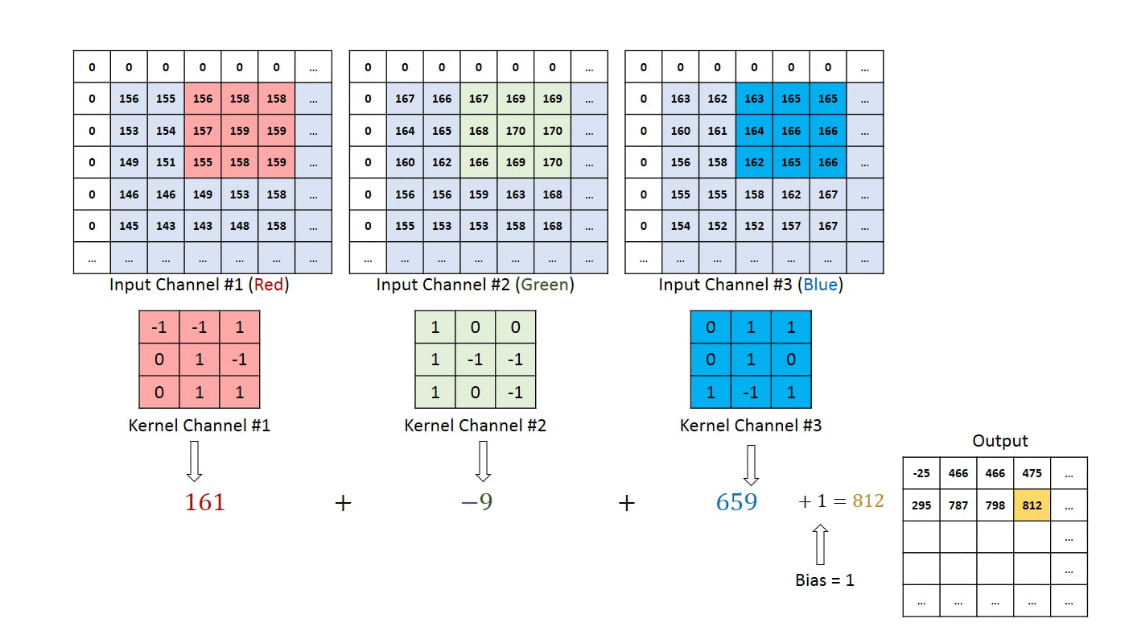
\includegraphics[scale=0.5]{images/ejemplo_convolucion_3canales}}
\caption{Aquí se puede ver un ejemplo de una convolución aplicada a una entrada con 3 canales, uno por cada color primario. Se ve cómo el kernel ahora tiene 3 canales también. Imagen extraída de \url{https://saturncloud.io/blog/a-comprehensive-guide-to-convolutional-neural-networks-the-eli5-way/}.}
\label{fig:ejemplo_convolucion_3canales}
\end{figure}

Ahora que ya está claro qué es una convolución, ya se puede definir una capa convolucional como una capa que aplica $n\in \mathbb{N}$ convoluciones a una entrada. Al número de convoluciones se le denomina \textbf{profundidad} y determina el número de canales que tendrá la salida de la capa. Las dimensiones espaciales de la salida dependerán de las dimensiones espaciales de la entrada y a las decisiones de \textit{padding} y \textit{stride} que se hagan. Además se aplica una función de activación, posición a posición, a la salida de la capa. Esta función habitualmente es la ReLU por las razones que ya se dieron en la subsección de funciones de activación.

El objetivo de las capas convolucionales es la detección de características locales de la entrada de la capa anterior ya que cada convolución aplica la misma operación localmente a lo largo de toda la entrada. Además, este tipo de capas tienen un número reducido de parámetros a aprender por la red ya que sólo hace falta aprender los pesos de los filtros.

\subsection*{Capas de pooling}

Las capas de \textit{pooling} se encargan de reducir las dimensiones espaciales de la entrada manteniendo el número de canales. Esto es, disminuyen el número de filas y columnas. Para ello dividen cada mapa de características en ventanas disjuntas que cubren todas las filas y columnas, y ``\textit{resumen}''  todos los valores en una ventana a uno sólo. Esto disminuye el coste computacional de la red. Este tipo de capas también busca juntar valores que son similares en uno sólo.

Los dos tipo típicos de \textit{pooling} son el \textbf{max pooling} que toma el máximo de los valores de la ventana y el \textbf{average pooling} que toma la media aritmética de los valores de la ventana. Se cree que \textit{max pooling} tiene mejor rendimiento y, de hecho, en la parte matemática de este TFG se pueden ver argumentos de por qué podría ser cierto. En la Figura \ref{fig:ejemplo_pooling} se puede ver un ejemplo de ambos tipos de \textit{pooling}.



\begin{figure}[h]
\noindent
\makebox[\textwidth]{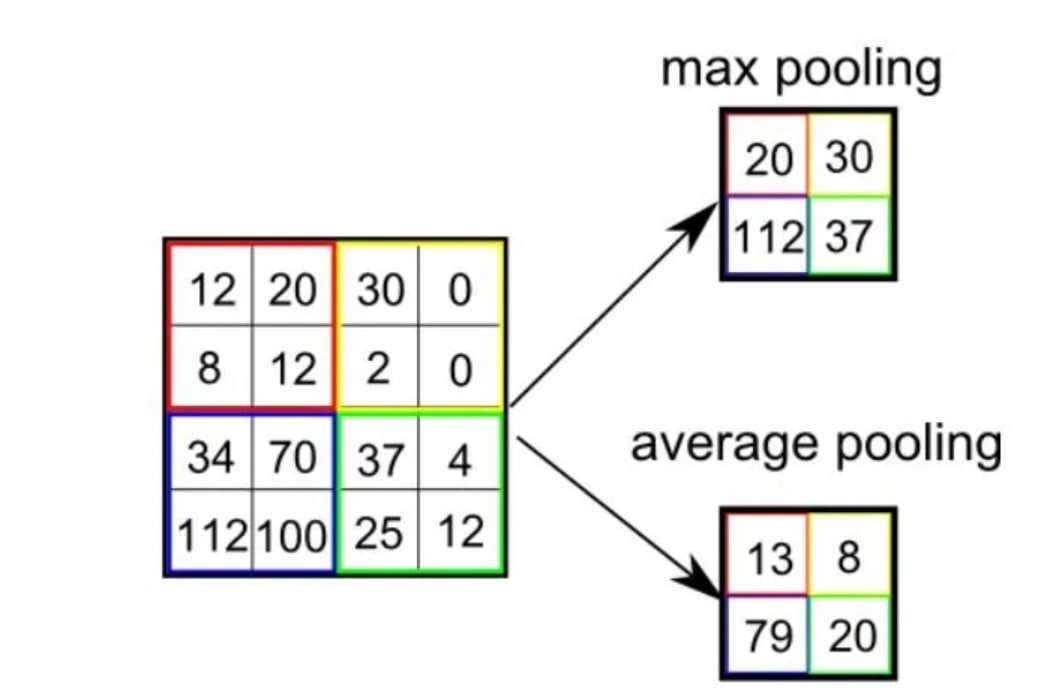
\includegraphics[scale=0.3]{images/ejemplo_pooling}}
\caption{En la figura se ver cómo se aplica \textit{max pooling} y \textit{average pooling} a una entrada. Como las ventanas tienen tamaño $2\times 2$ se dice que se aplica \textit{pooling} $2\times 2$. Imagen extraída de \url{https://saturncloud.io/blog/a-comprehensive-guide-to-convolutional-neural-networks-the-eli5-way/}.}
\label{fig:ejemplo_pooling}
\end{figure}

\subsection*{Capas totalmente conectadas}
Este tipo de capas no son más que una capa típica de MLP que conecta todos los valores de las neuronas de la capa anterior con todas las neuronas de esta capa. Se colocan después de todas las capas convolucionales de \textit{pooling}. Por ejemplo, si se quisiera resolver un problema de clasificación de imágenes en cinco clases, se tendría una última capa totalmente conectada con cinco neuronas.


\section{XAI}

Los modelos de ML se pueden dividir en dos tipos: los \textbf{modelos de caja negra} (\textit{black-box models}) y \textbf{modelos de caja blanca} (\textit{white-box models}) \cite{XAIWHATWEKNOW, XAINOTIONS}.

 Los modelos de caja blanca producen resultados que pueden ser interpretados por los usuarios o expertos que utilizan el modelo, normalmente mirando sus parámetros. Los modelos primitivos de ML, como la regresión lineal, regresión logística o árboles de decisión, suelen ser de este tipo. 
 
Por otro lado los modelos de caja negra son modelos difíciles de interpretar y explicar debido a que tiene estructuras complejas, con una gran cantidad de parámetros y no lineales. Los modelos más importantes pertenecientes a esta clase son las ANNs. 

Algunos trabajos incluyen una categoría conocida como \textbf{modelos de caja gris} (\textit{gray-box models}), los cuales son modelos que se pueden interpretar, al menos parcialmente, si se diseñan adecuadamente.


La \textbf{Inteligencia Artificial eXplicable} (\textit{eXplainable Artificial Inteligence, XAI}) \cite{XAIManifesto, XAIWHATWEKNOW, XAINOTIONS, XAICONCEPTS} es un campo de estudio que pretende desarrollar métodos para construir modelos de ML que aumenten la interpretabilidad de estos sin que esto afecte demasiado a su rendimiento. Para ello hay caminos:

\begin{itemize}
\item Construir modelos de caja blanca o gris con rendimientos altos.
\item Dotar a los modelos de caja negra de un mayor nivel de interpretabilidad.
\end{itemize}

En XAI, la \textbf{Interpretabilidad} se refiere a la capacidad de comprender cómo los modelos de IA toman sus decisiones. Por otro lado la \textbf{explicabiliad} se refiere a la capacidad de hacer interpretaciones y describir el funcionamiento interno de un sistema de IA en términos humanos. Estos dos son los dos principales criterios a la hora de evaluar métodos de XAI, además de ellos existen otros como \textbf{transparencia}, \textbf{justicia} (\textit{fairness}) y \textbf{robustez}. 

En general el objetivo de la explicabilidad es hacer algún aspecto del modelo entendible para el usuario. Si lo que se intenta hacer expllicable es una salida del modelo para una instancia, se habla de \textbf{explicabilidad local}. En cambio si es el dataset entero se habla de \textbf{explicabilidad global}.

Una distinción en los métodos de XAI es si el método es \textit{\textbf{ante-hoc}} o \textit{\textbf{post-hoc}}. Los métodos \textit{ante-hoc} son aquellos que entrenan un método explicable en primer lugar. Por otro lado los \textit{post-hoc} pretenden explicar un modelo de caja negra después de ser explicado. A su vez, los métodos \textit{post-hoc} se dividen en métodos \textbf{agnósticos al modelo} si funcionan para cualquier modelo, y métodos \textbf{específicos al modelo} si sólo funcionan para un tipo (o clase) de modelos.

Por último está la siguiente distinción de métodos según la metodología que utilicen: \textbf{basados en retropropagación} y \textbf{basados en perturbaciones}. Los que se basan en retropropagación propagan una señal de la salida del modelo hacia la entrada. Los basados en perturbaciones modifican la entrada del modelo utilizando distintas técnicas para investigar el impacto de estas modificaciones en la salida del modelo.


\subsection{Explicaciones lineales locales y LIME} \label{subsec:LIME}

Las \textbf{Explicaciones lineales locales} (\textit{Linear Local Explanation, LLE}) \cite{REVEL,LIME} son una clase de explicaciones para modelos de caja negra.

 Sea $X \subset \mathbb{R}^F$ el datatset de entrada, siendo $F$ el número de características por ejemplo, y sea $f : \mathbb{R}^F \rightarrow \mathbb{R}^C$ la función que implementa un modelo de caja negra, dónde $C$ es el número de clases de un problema de clasificación al que se aplica. Sea $x\in X$ una entrada a ser explicada. Un explicador LLE de caja blanca es una función $g: \mathbb{R}^F \rightarrow \mathbb{R}^C$ definida como:
 
\begin{equation}
g(x) = Ax + B, \quad A \in \mathcal{M}_{F,C}, B \in \mathbb{R}^C
\end{equation}

Dónde $\mathcal{M}_{F,C}$ es el conjunto de todas las matrices con $F$ filas y $C$ columnas. Es decir, $g$ no es más que una función lineal que lleva una entrada del modelo al espacio de salida del modelo. Este modelo se puede interpretar pues intuitivamente para cada peso $a_{i,j}$ de $A$ denota la importancia que tiene la característica de entrada $i$ con la predicción de la salida $j$. Por otro lado cada valor $b_j$ del vector $B$ está conectado con la importancia en general de la salida $j$.

Para obtener la función $g$ anterior los métodos LLE utilizan regresión lineal sobre una vecindad del ejemplo $x$. El error que minimizan es el siguiente:

\begin{equation}
\mathcal{L}(f,g,\pi_x) = \sum_{z \in N(x)} \pi_x(z)(f(z)-g(z))^2
\end{equation} 

Nótese que esto no es más que el error cuadrático medio ponderando cada vecino por una función $\pi_x$ que mide la proximidad a $x$ para cada vecino generado $z$, que dependerá del LLE utilizado.  Aquí $N(x)$ representa el vecindario de $x$ para el número de vecinos generados es un parámetro del LLE.


El método de \textbf{explicaciones locales interpretables agnósticas al modelo} (\textit{Local Interpretable Model-agnostic Explanations, LIME}) \cite{REVEL,LIME} es una técnica LLE considerada como estado del arte. En LIME se realiza una regresión de cresta (\textit{Ridge regresion}) para obtener $g$, definiendo la $\pi_x(z)$ como sigue:

\begin{equation}
\pi_x(z) = e^{\frac{-d(x,y)^2}{\sigma^2}}
\end{equation}

dónde $d(\cdot,\cdot)$ es la distancia euclídea (en el caso de imágenes) y $\sigma$ es un factor de regularización.

Para la generación de vecinos en $N(x)$ se muestrea un valor $v'$ de la distribución exponencial $Exp(\lambda)$ con $\lambda = \frac{1}{\sigma}$. Después se toma $v = \min\{\lfloor v' \rfloor, F\}$. El valor $v$ determina cuantas características de $x$ se van a ocluir. Estas se escogen de forma aleatoria (uniformemente).

La elección de lo que es una característica depende del tipo de dato con el que se trate. En el caso de este TFM se trata con imágenes. Para las imágenes se puede tratar cada pixel individualmente como una característica. Sin embargo esto hace que haya muchas características lo que hace que generar este tipo de explicaciones sea caro. Además desde un punto de vista humano un pixel individual no suele tener un significado específico en una imagen, es más natural que un conjunto de pixeles tengan un significado. Por ello consideramos una división de la imagen en cuadrados del mismo tamaño y cada uno de ello conlleva una característica.

\subsection{Métricas ReVEL} \label{subsec:revel}

El framework \textbf{Evaluación robusta vectorizada de explicaciones-lineales-locales} (\textit{Robust Evaluation VEctorized Loca-linear-explanation, REVEL}) \cite{REVEL} ofrece un análisis robusto y consistente de explicaciones LLEs generadas para modelos de caja negra. En este se presentan cinco métricas que miden distintos aspectos cualitativos de la explicación. 

Antes de introducir estás métricas introduzco algunas matrices antes. Nos situamos en un problema de clasificación en el que hemos entrenado un modelo de caja negra, sea $g$ una explicación generada por un LLE, tal que $g: F \rightarrow Y_l$ dónde $Y_l$ es el espacio \textit{logit}. Este espacio no es más que la salida del modelo de caja negra antes de aplicar la función \textit{softmax} que transforma la salida del modelo a probabilidades de cada clase. Recordar que $g(x) = Ax + B$. 

Se define la \textbf{matriz de importancia con signo}, $A^l$ como la matriz derivada sobre el espacio \textit{logit}. Como es evidente al ser lineal $A^l = A$. Por otro lado, para la obtención del vector de probabilidades $p$ se necesita aplicar la función \textit{softmax} a $g(x)$ luego $p=softmax(g(x))=softmax(Ax+B)$. Se define la matriz $A^p = D(softmax(g(x)))(x)$ siendo $D(\cdot)$ el operador derivada. La función $softmax$ es la función que para clase $c$ se define como:

\begin{equation}
softmax(y_1,y_2,...,y_C)_c = \frac{e^{y_c}}{\sum_{i=1}^C e^{y_i}}
\end{equation}
 
La forma de interpretar estas dos matrices es teniendo en cuenta que el elemento en la fila $i$ y columna $j$ de cada matriz representa la importancia de la característica $i$ sobre la clase $j$ sobre los espacios \textit{logit} y \textit{probabilidad}. Por un lado $A^l$ da información sobre como afecta, positiva o negativamente dependiendo del signo, cada característica a los distintos \textit{logits} de las clases. Por otro lado, $A^P$ proporciona información sobre las clases en las que el ejemplo es más probable de ser clasificado.

Como ambas matrices presentan información relevante se define la \textbf{matriz de importancia} como la matriz que combina la información de $A^l$ y $A^p$ como sigue:

\begin{equation}
A_{i,j} = sign(A^l_{i,j}) \sqrt{|A^l_{i,j}|\cdot|A^p_{i,j}|}
\end{equation}

A partir de esta matriz se define la \textbf{matriz de importancia normalizada} $A_r=\frac{A}{ max_{A_{i,j}}\{|A_{i,j}|\} }$ que lleva los valores de $A$ al rango $[-1,1]$ manteniendo su signo. Finalmente se define la \textbf{matriz de importancia absoluta} como la matriz $|A|$ que simplemente es la matriz $A_r$ con todos sus elementos en positivo. 

\highlight{Leyendo tu artículo no me queda claro si la matriz de importancia absoluta es $|A_z|$ o $|A|$}

Ya estamos en condiciones de introducir las cinco métricas introducidas en REVEL. De aquí en adelante $g(x)$ se toma en el espacio de probabilidades, no en el de \textit{logit}.

\subsubsection*{Local concordance}

Se define como:

\begin{equation}
Local\_Concordance(g) =  1 - \frac{||f(x)-g(x)||}{C'}
\end{equation}

Dónde $||\cdot||$ es una norma arbitraria (por ejemplo la norma euclídiana $||\cdot||_2$) y $C'$ es la distancia máxima posible entre dos vectores de probabilidad (por ejemplo en el caso de $||\cdot||_2$ se cumple que $C'=\sqrt{2}$). 

Notemos que esta métrica está definida en el intervalo $[0,1]$ dónde el valor máximo se alcanza cuando $f(x) = g(x)$ y la mínima ocurre cuando ambas funciones clasifican $x$ en clases distintas con probabilidad 1.

Esta métrica mide cómo de similar es la explicación al ejemplo original de la caja negra. Es importante que esté cercana a 1 ya que en otro caso la explicación propuesta no se corresponde con el ejemplo escogido.

\subsubsection*{Local fidelity}

Se define como:

\begin{equation}
 Local\_Fidelity(g) =  \frac{1}{|N(x)|} \sum_{z\in N(x)} 1 - \frac{||f(z)-g(z)||}{C'}
\end{equation}

Dónde $|N(x)|$ es el número de vecinos generados para la explicación. 

Esta métrica se puede ver como la media de la métrica anterior sobre los vecinos de $x$, por lo tanto también está definida en el intervalo $[0,1]$. Esta métrica mide cómo de cercan están las probabilidades calculadas por el modelo de caja blanca de las que calcula el modelo de caja negra. Luego mide la similitud entre la explicación y el modelo $f$ en la vecindad de $x$. Al igual que pasaba con la \textit{local concordance}, debe ser cercano a 1 para obtener buenas explicaciones.

\subsubsection*{Prescriptivity}
Se define como:

\begin{equation}
Presciptivity(g) =  1 - \frac{||f(x+h)-g(x+h)||}{C'}
\end{equation}

Dónde $h$ es una perturbación sobre $x$ que quita la presencia de las características más importantes (de forma positiva) de la clase asignada por $g$ al ejemplo $x$. De esta forma, para encontrar $h$ se van quitando dichas características hasta que se cumpla que $argmax(g(x))\neq argmax(g(x+h))$.

Notemos que esta métrica también está contenida en $[0,1]$ y obtiene el valor 1 cuando $f(x+h)=g(x+h)$ y obtiene el valor 0 cuando ambas funciones clasifican $x+h$ en clases distintas con probabilidad 1.

Esta métrica pretende estudiar si la explicación $g$ es capaz de predecir correctamente los cambios necesarios en el ejemplo $x$ para cambiar la clase original. Para ello busca un valor lo suficientemente alejado del ejemplo para que la explicación cambie la clase predicha y mida cómo cambia la predicción respecto del modelo de caja negra. Al contrario que las dos métricas anteriores un valor cercano a 1, aunque buscado, no es necesario para obtener buenas explicaciones.

\subsubsection*{Conciseness}
Se define como:

\highlight{Aquí he adaptado la fórmula de \href{tu artículo}{https://arxiv.org/abs/2211.06154} con la información de la documentación de tu código en github para que quede más claro (a mi me queda más claro).} 

\begin{equation}
Conciseness(g) =  \frac{1}{f'-1} \sum_{i=1}^{f'} 1-I_i \\
\end{equation} 



Dónde $f'$ es el número de filas de la matriz de importancia absoluta (equivalentemente, número de clases), sea $v_i$ el vector fila $i$ de la matriz $|A|$ entonces:
\begin{equation}
I_i = \frac{||v_i||}{max_{1\leq  j \leq f'}\{||v_j||\}}
\end{equation}

Observemos que $v_i$ es un vector en que cada elemento $j$ representa la importancia de la característica $i$ para la clase $j$ luego se puede interpretar que $I_i$ es la importancia de dicha característica (normalizada a $[0,1]$). Si analizamos la expresión de la métrica tenemos que esta está comprendida entre $[0,1]$ y alcanza 1 si una métrica tiene importancia 1 y el resto tiene importancia 0. Si todas las características tuvieran la misma importancia, por estar $I$ normalizada serían todas 1 y se obtendría el menor valor posible en 0.

Esta métrica busca medir la brevedad de la explicación, es decir, cuantas menos características sean relevantes para la explicación, más concisa se considera la explicación. Luego mide la habilidad de la explicación de concentrarse en las características importantes. Al contrario que las métricas anteriores, dependiendo de la tarea se podría querer más o menos \textit{conciseness} ya que valores demasiados bajos podrían indicar que el modelo se centra en cosas irrelevantes (por ejemplo en imágenes que se centre en pocos píxeles podría ser malo).

\subsubsection*{Robustness over explanations}

Se define como:

\begin{equation}
Robustness(G) =  \mathbb{E}[similarity(g,g')]
\end{equation}

Dónde $G$ representa el conjunto de todas las explicaciones que podría generar el LLE, $\mathbb{E}$ es la esperanza y $similiarity$ es una función que mide cuanto difieren dos explicaciones distintas y se define como:

\begin{equation}
similarity(g,g') = \left(\frac{A_r\cdot A'_r}{||A_r|| ||A'_r||} \right)  \left(1-  \frac{|\quad  ||A_r||-||A'_r|| \quad |}{max\{||A_r||,||A'_r||\}}\right)
\end{equation}

Observemos que la componente de la derecha mide cómo de similares son las magnitudes de las las matrices de importancia absoluta normalizadas de las explicaciones mientras que el valor de la izquierda se corresponde con la similaridad coseno entre $A_r$ y $A_r'$ (matrices correspondientes con $g$ y $g'$ correspondientemente), esta mide como distan las direcciones de las explicaciones. El producto de matrices de esta función es el elemento a elemento. El mejor caso, cuando ambas explicaciones son iguales, se tiene que la similaridad es 1 y el peor caso ocurre son ``perpendiculares'' y la similaridad es 0. 

En la práctica, para aproximar la \textit{Robustness} se hace la media de la similaridad generando muchas otra explicaciones $g'$ para $x$. Esto únicamente se puede hacer para LLEs que no son deterministas, pues en otro caso siempre se tendría la misma explicación y obtendrían siempre 1. Por ejemplo con LIME sí se puede calcular esta métrica pues tiene no determinismo en la generación de la vecindad.


Esta no es una métrica sobre la explicación en específico sino sobre el método que las genera. Cuanta más cercana a 1 menos varían las explicaciones generadas por el método estudiado. Esta métrica al contrario que todas las anteriores puede obtener valores negativos, lo que indicaría explicaciones que se ``contradicen''.

\subsection{Regularización X-Shield} \label{subsec:XSHIELD}

La \textbf{regularización} \cite{XSHIELD, Regularization} es la modificación de la arquitectura del modelo, del proceso de aprendizaje o inferencia para imponer algún criterio sobre este. Por ejemplo, dropout, que ya se vió previamente, es una regularización. 

En particular nos interesan las regularizaciones que implican añadir a la función de coste un nuevo término que indica el criterio que queremos minimizar en el modelo. Algunos ejemplos típicos son la regularización L1 o L2. En general se tiene que una regularización de este tipo se expresa como:

\begin{equation}
coste\_regularizado(\Theta, X, Y) = coste(f_\Theta (X), Y) + regularizacion(X,\Theta )
\end{equation}

Dónde se tiene que $\Theta$ son el conjunto de parámetros del modelo, $X$ son las entradas del conjunto de datos y $Y$ las salidas. Por lo tanto la regularización es una función que puede ser de los parámetros y de las datos de entrada.

En primer lugar presentamos la familia de regularizaciones \textbf{\textit{Transformation-Selective Hidden Input Evaluation for Learning} ,T-SHIELD} \cite{XSHIELD}. Esta esta diseñada para hacer que el modelo aprenda con menos features. Para ello se ocluye parte de la entrada. 

Para ello se utiliza una transformación $T: \mathbb{R}^F \rightarrow \mathbb{R}^F$ tal que $T(x)_i = x_0$ si $i$ es una característica a esconder y $T(x)_i = x_i$ si no lo es. Es decir está transformación cambia todas las características de una entrada $x$ por un valor constante $x_0$ y deja el resto intactos.

Para una transformación $T$ como la anterior descrita, se define la regularización T-SHIELD como sigue:

\begin{equation}
T-SHIELD(x,\Theta) = KL(f_\Theta(T(x)),f_\Theta(x)) + KL(f_\Theta(x),f_\Theta(T(x))) 
\end{equation}

Dónde $KL(\cdot,\cdot)$ denota la distancia de Kullback-Leibler, que se trata de un tipo de distancia que mide como difieren dos distribuciones distintas. Por lo tanto esta regularización no es más que la distancia de Kullback-Leibler simétrica. Según como se construya la transformación $T$ esta regularización penalizará ciertos aspectos del modelo. En la Figura \ref{fig:tshield_flow} se puede ver cómo funcionaría una regularización de esta familia de forma general.

\begin{figure}[h]
\noindent
\makebox[\textwidth]{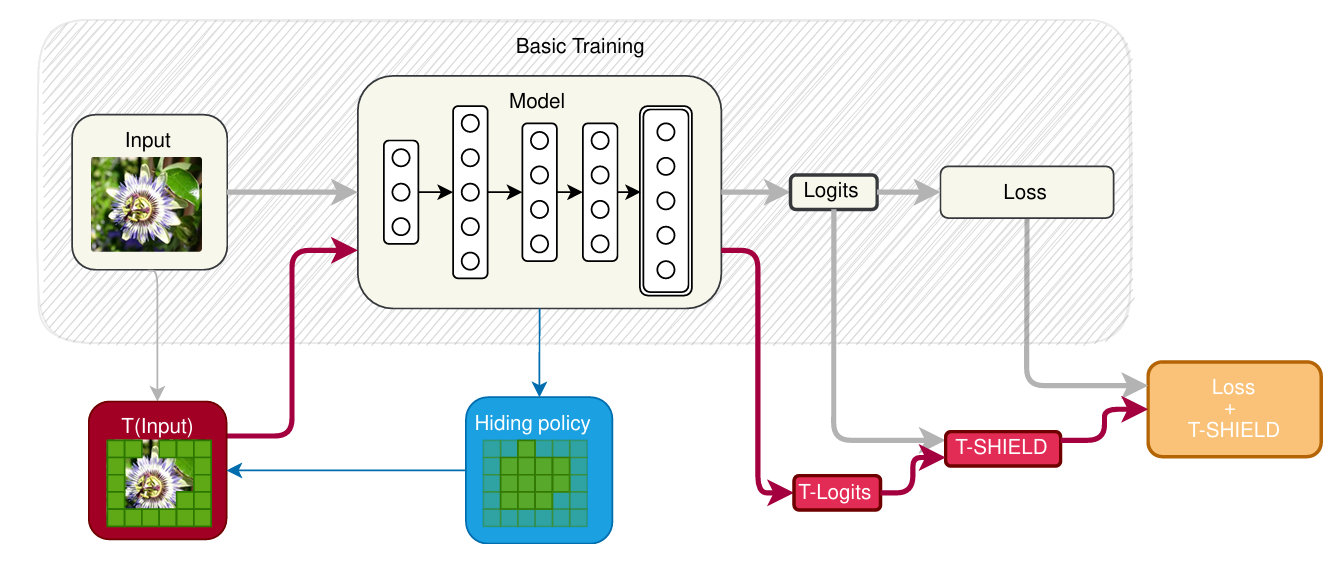
\includegraphics[scale=0.5]{images/tshield_flow}}
\caption{ En esta figura se puede ver cómo funciona en general la familia de regularizaciones T-SHIELD durante el entrenamiento. En gris se puede ver el flujo normal de la imagen en el modelo. En azul se encontraría la forma en la que la regularización decide qué características ocluir. Finalmente en rojo se encontraría el flujo de la imagen con las características ya ocluidas y cómo se calcula la función de regularización. Imagen extraída de \cite{REVEL}.}
\label{fig:tshield_flow}
\end{figure}

Se denomina \textbf{Random-SHIELD (R-SHIELD)} a la regularización de la familia T-SHIELD que para un parámetro $\lambda \in [0,100]$ define la transformación $T$ como aquella que esconde un $\lambda\%$ de las características de forma aleatoria (misma probabilidad para cada una).

\begin{figure}[h]
\noindent
\makebox[\textwidth]{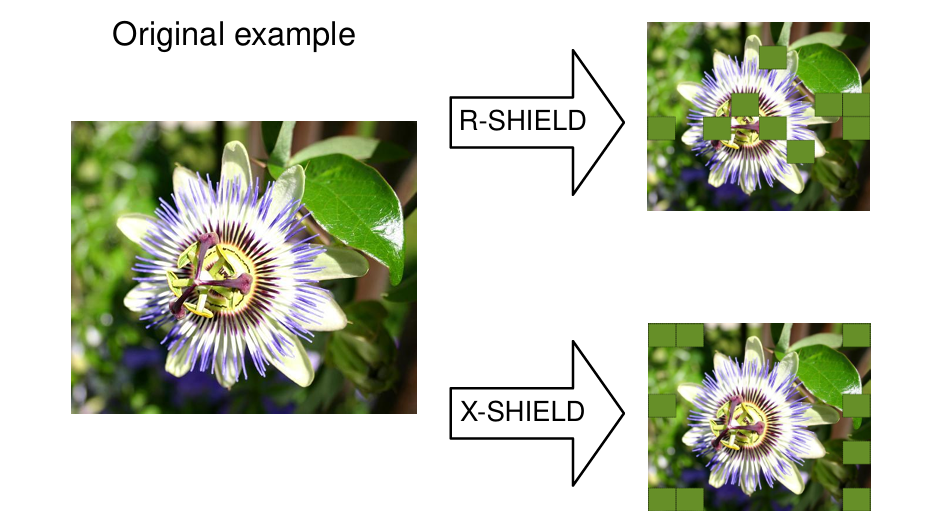
\includegraphics[scale=0.5]{images/rshield_vs_xshield}}
\caption{ Comparación entre el comportamiento de $T$ en R-SHIELD y X-SHIELD. La imagen está sacada del dataset \textit{Flowers} de clasificación de imágenes de flores. Se puede ver que R-SHIELD ocluye partes de la imagen aleatorias, incluyendo partes de la flor a clasificar. Por otro lado X-SHIELD ocluye partes del fondo de la imagen que intuitivamente no parecen útiles para clasificar dicha flor. Imagen extraída de \cite{REVEL}.}
\label{fig:rshield_vs_xshield}
\end{figure}


Se denomina \textbf{XAI-SHIELD (X-SHIELD)} a otra regularización de la familia T-SHIELD. Comparte el parámetro $\lambda$ de R-SHIELD pero en vez de ocultar el $\lambda\%$ de características aleatorias, va a ocultar las $\lambda\%$ menos importantes. Para ello, a cada característica le otorga la importancia $||v_i||$ donde $v_i$ es la fila $i$ de la matriz de importancia $A$ introducida en la subsección \ref{subsec:revel}, pero para el modelo que se está entrenando.

De manera más formal se describe $T_{xai}(x;\lambda)$ como la transformación:

\begin{equation}
T_{xai}(x_1,...,x_F; \lambda) = (\underbrace{x_0,x_0...,x_0,x_0}_{0 \leq i\leq F : \quad \lambda < \frac{i}{n}\cdot 100\%},x_i,x_{i+1},....,x_F)
\end{equation}



Dónde se ha supuesto los atributos $x_i$ ordenados de menor a mayor por importancia y tenemos que $i$ es el menor valor tal que se ocluyen al menos el $\lambda \%$ de características.



En la Figura \ref{fig:rshield_vs_xshield} se puede apreciar la diferencia entre los comportamientos de los dos tipos de regularización T-SHIELD vistos.




\newpage
\chapter{Estado del arte} \label{cap:eda}
Este Trabajo de Fin de Máster trata de resolver el problema de construir un modelo de IA de clasificación para lesiones cancerosas en biposias de próstata y de la mejora en interpretabilidad del modelo mediante técnicas de XAI. Por lo tanto vamos a hacer una revisión del estado del arte para los cuatro siguientes puntos que son relevantes:


\begin{itemize}
\item Redes convolucionales para clasificación de imágenes.
\item Métodos de XAI para producción de explicaciones, en particular, LLEs.
\item Métodos de XAI de regularización para mejoras las explicaciones.
\item Métricas de XAI de calidad de las explicaciones producidas para poder comparar los distintos métodos utilizados.
\end{itemize}

\subsection*{Modelo de clasificación}

\textbf{Efficientnet} \cite{efficientnet2019} es una red introducida en 2019 que se sigue considerando estado del arte en clasificación de imágenes cuando se mide eficiencia computacional, es decir, rendimiento obtenido número de parámetros. En la Figura \ref{fig:efficientnet_grafica} se puede apreciar como es más eficiente en cómputo respecto otros modelos de clasificación de imágenes ResNet \cite{resnet} o DenseNet \cite{densenet} para el dataset Imagenet. 

Existen otros modelos más modernos como CoCa \cite{coca}, DaViT \cite{DaViT} o ConvNeXt V2 \cite{ConvNext}, que utilizan transformadores en el caso de Coca y DaViT, o autoencoders en el caso de ConvNeXt V2. Estos modelos alcanzan precisiones mayores que EfficientNet sin embargo aumentan demasiado el número de parámetros utilizado para que sea una propuesta viable para nuestro trabajo.

Por ello hemos decidido utilizar el modelo EfficientNet en este trabajo ya que ofrece un balance muy bueno entre número de parámetros y precisión. En la Tabla \ref{tab:comparacion_modelos_efficientnet} se puede apreciar las diferencias entre el modelo que utilizaremos EfficientNet-B2 y las versiones más pequeñas de los modelos mentados. Se aprecia que EfficientNet es más eficiente en el número de parámetros.

\begin{table}[ht]
\centering
\begin{tabular}{|l|l|c|c|}
\hline
\textbf{Modelo} & \textbf{Arquitectura Base} & \textbf{Parámetros (M)} & \textbf{Precisión Top-1 (\%)} \\
\hline
EfficientNet-B2 & CNN & 9.1 & 80.1 \\
DaViT-Small     & CNN + Transformer & 49.7 & 84.2 \\
ConvNeXt V2-Tiny & CNN moderna (con Masked Autoencoder) & 28.6 & 85.1 \\
CoCa-Base & Transformer & 383 & 91.0 \\
\hline
\end{tabular}
\caption{Comparación de modelos en términos de precisión Top-1 en ImageNet y número de parámetros.}
\label{tab:comparacion_modelos_efficientnet}
\end{table}


\begin{figure}[h]
\noindent
\makebox[\textwidth]{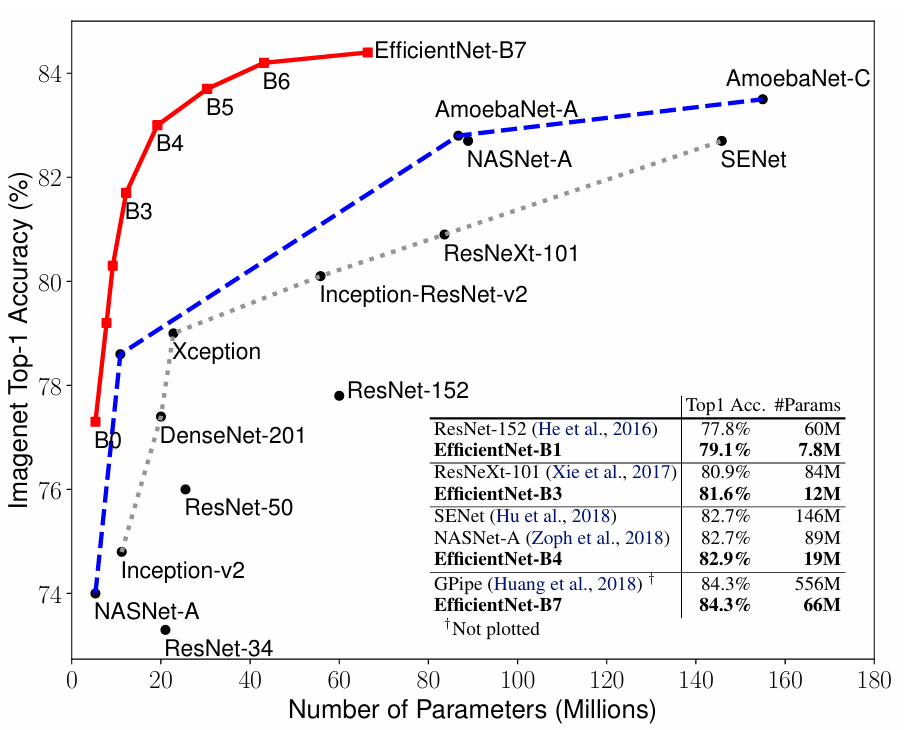
\includegraphics[scale=0.75]{images/Efficientnet_grafica}}
\caption{En esta gráfica se compara las distintas versiones de Efficientnet, B0-7, contra otros modelos de redes convolucionales. Se puede apreciar que es la más eficiente. Imagen extraída de \cite{efficientnet2019}.}
\label{fig:efficientnet_grafica}
\end{figure}



\subsection*{Métodos de XAI para producción de explicaciones}

Una revisión de todos los métodos de explicabilidad \textit{post-hoc}, que son los que se aplican a modelos de caja negra, está fuera de el alcance de este trabajo pues sería inabarcable. Sin embargo resumimos algunos métodos populares (esquema en la Tabla \ref{tab:xai_explicaciones}):

\begin{itemize}
    \item \textbf{LIME} \cite{LIME}: Modelo explicado con detalle en la subsección \ref{subsec:LIME}.
    
    \item \textbf{SHAP} (\textit{SHapley Additive exPlanation}) \cite{SHAP}: Basado en valores de Shapley de teoría de juegos. Atribuye importancia a cada variable de forma consistente; permite explicaciones locales y globales. 
    
    \item \textbf{LRP} (\textit{Layer-wise Relevance Propagation}) \cite{LRP}: Propaga hacia atrás la relevancia de la predicción a través de cada capa de la red. Muy usado en visión y señales neuronales. 
    
    \item \textbf{CRP} (\textit{Concept Relevance Propagation}) \cite{CRP}: Extiende LRP incorporando información contextual o conceptual. Promete explicaciones más interpretables en términos humanos. 
    
    \item \textbf{Grad-CAM} (\textit{Gradient-weighted Class Activation Mapping}) \cite{Gradcam}: Técnica visual para CNNs que genera mapas de calor mostrando qué regiones de una imagen influyen en la clasificación. 

    \item \textbf{Integrated Gradients} \cite{IntGradients}: Método axiomatizado de atribución que compara la entrada con una baseline. Proporciona asignaciones más estables que gradientes simples. 
    

\end{itemize}


\begin{longtable}{|p{3.5cm}|p{3.5cm}|p{3.5cm}|}
\hline
\textbf{Técnica} & \textbf{Tipo} & \textbf{Enfoque} \\
\hline
\endfirsthead
\hline
\textbf{Técnica} & \textbf{Tipo} & \textbf{Enfoque} \\
\hline
\endhead

\textbf{LIME} & Modelo-agnóstico & Local \\
\hline

\textbf{SHAP} & Modelo-agnóstico  & Local y Global  \\
\hline

\textbf{LRP} & Modelo-específico (DNN) & Local \\
\hline

\textbf{CRP / Concept R.P.} & Modelo-específico (DNN) & Local\\
\hline

\textbf{Grad-CAM (+ variantes)} & Modelo-específico (CNNs) & Visual  \\
\hline

\textbf{Integrated Gradients} & Modelo-específico (DNN) & Local (atribución) \\
\hline

\caption{En esta tabla se muestran algunas técnicas clave de XAI.}
\label{tab:xai_explicaciones}
\end{longtable}

En este estudio nos hemos dejado muchos métodos como explicaciones por ejemplos (como generación de \textit{counterfactuals} \cite{counterfactuals}) o las muchas extensiones de los métodos mentados (por ejemplo para LIME en \cite{LIMESURVEY} hay una taxonomía de estos).


\subsection*{Métricas para explicaciones}

Debido a que hay muchos tipos de explicaciones en la literatura (LLEs, mapas de atribución, reglas...) no hay manera de comparar estas directamente. Debido a esto, se existen distintas métricas para medir de forma cuantitativa la calidad de las explicaciones.

En \cite{metricasReglas} se proponen cuatro métricas para medir la calidad de explicaciones. Sin embargo estas son específicas para explicaciones basadas en reglas. Las métricas que representan son:
\begin{itemize}
\item $D$: la diferencia en rendimiento entre el modelo a explicar y la explicación basada en reglas. Cuantifica el cambio entre el modelo de caja negra y el mejor modelo de caja blanca observado.
\item $R$: El número de reglas de la explicación. Busca cuantificar lo simple que es la explicación.
\item $F$: El número de características que se han utilizado para construir la explicación. Es similar a $R$, cuanto menor es mejor se considera la explicación.
\item $S$: La estabilidad de la explicación. Cuantifica la habilidad de la explicación de manejar robustamente perturbaciones pequeñas.
\end{itemize} 

En \cite{LEAF} se propone el framework \textit{LEAF}. En este se introducen 5 métricas para evaluar de forma clara las explicaciones de LLEs. Las métricas son las siguientes:

\begin{itemize}
\item \textit{Conciseness: }se interpreta como hasta qué punto el modelo es entendible por un humano. Se define como el número de pesos de la explicación (es una LLE) son no nulos.
\item \textit{Local Fidelity: }mide el modelo de caja blanca $g$ (la explicación) aproxima el comportamiento del modelo de caja negra $f$ para un ejemplo $x$ y su vecindad $N(x)$. Este se calcula con el \textit{F1-score} sobre dicha vecindad y dependerá por lo tanto de cómo se muestree esta. 
\item \textit{Local Concordance: }mide como $g$ aproxima a $f$ justo en el ejemplo $x$. Se mide como $max\{0, 1-|f(x)-g(x)|\}$.  
\item \textit{Reiteration Similarity: }muchos métodos de LLEs utilizan aleatoriedad para generar sus explicaciones. Debido a esto aplicar muchas veces un algoritmo para generar una explicación para un mismo ejemplo $x$ puede generar explicaciones distintas cada vez. Se propone esta métrica para medir la similaridad del conjunto de explicaciones generadas. Esta se calcula como la similaridad de \textit{Jaccard} $J$ esperada entre dos explicaciones $g$ y $g'$. Es decir $\mathbb{E}[J(g,g')]$.
\item \textit{Prescriptivity: }mide en qué medida una explicación local puede usarse para modificar una instancia y cambiar su clasificación. Se calcula proyectando $x$ sobre la frontera de decisión del modelo explicativo $g$, y evaluando qué tan cerca está esa proyección del límite. Sea $x'$ dicha proyección entonces se calcula como la pérdida \textit{hinge} normalizada de $f(x')-g(x')$.
\end{itemize}

Finalmente, en \cite{REVEL} se introducen las métricas REVEL, que ya hemos introducido en \ref{subsec:revel}. Este framework propone cinco métricas al igual que LEAF. REVEL está compuesto de las mismas 5 métricas, cambiando \textit{Reiteration Similarity} por \textit{Robustness} que busca medir lo mismo. Sin embargo REVEL cambia cómo se calcula cada una de las métricas introduciendo mejoras en todas ellas. Es por esto por lo vamos a utilizar en este trabajo estas métricas para medir la calidad de nuestras explicaciones.

\highlight{¿Debería ir una por una explicando las mejoras de las métricas REVEL respecto a LEAF?}



\subsection*{Métodos de regularización XAI}

Los métodos de regularización en XAI \cite{XSHIELD, EstadoArteMetodos}, que añaden un término regularizador a la función de pérdida, plantean una manera sencilla para modificar el comportamiento del modelo, favoreciendo criterios buscados. Estos son por construcción agnósticos al modelo, aunque algunos requieren que  este sea diferenciable, y sencillos de implementar. Por ello son uno de los métodos más estudiados en la técnicas de XAI.

En \cite{RRR} se introduce \textit{Right for the Right Reasons} (RRR) que busca optimizar el razonamiento del modelo. En este trabajo el conjunto de datos $X$, a parte es estar etiquetado, debe proveer una máscara en la que se indique si cada dimensión de la entrada debe ser relevante o irrelevante para la decisión. En este trabajo las explicaciones se hacen mediante el gradiente respecto el logaritmo de la salida del modelo. 

En \cite{REGINPUTGRAD} se realiza un método similar al anterior, pero solucionan el problema de la anotación manual de los datos para determinar qué parte de las entradas son irrelevantes. En este se generan perturbaciones de la entrada y se calcula sus mapas de atribución. El componente regularizador penaliza cambios significativos en las explicaciones. Este método busca que las explicaciones sean más estables y robustas. 

En \cite{simpleregularizacion} se introduce \textit{Contextual Decomposition Explanation Penalization} (CDEP). Este utiliza la diferencia absoluta entre la explicación producida y la explicación dada por un experto. Para ello, se emplea el método \textit{Contextual Decomposition} (CD) como técnica de atribución, que permite calcular explicaciones diferenciables durante el entrenamiento. De esta forma, se penaliza directamente en la función de pérdida cualquier discrepancia entre el razonamiento del modelo y el conocimiento previo.

Finalmente, en \cite{XSHIELD} se introduce X-SHIELD el método del que partimos. Este método no tiene restricciones teóricas sobre la entrada, salida o tarea que realiza el modelo, sólo que el modelo sea diferenciable. Está probado que este mejora el rendimiento en las métricas REVEL, que son las utilizadas en este trabajo, lo que nos proporcionará un método base con el que comparar nuestras propuestas. XSHIELD también ha demostrado que es capaz de aumentar no sólo las métricas REVEL sino que también mejora en muchos casos el rendimiento en clasificación del modelo.


\newpage
\chapter{Métodos} \label{cap:met}

\section{EfficientNet}

El modelo de clasificación de imágenes que vamos a entrenar sobre nuestro conjunto de datos y sobre el que aplicaremos las distintas regularizaciones XAI se trata de \textbf{EfficientNet} \cite{efficientnet2019}. EfficientNet es una familia de CNNs muy eficiente en rendimiento, obteniendo buenos resultados en accuracy versus número de parámetros presentes en la red (Figura \ref{fig:efficientnet_grafica}). Esto hace que sea muy versátil y se adapte al poder de computo del que disponemos. Además la precisión final obtenida por la red, aunque es relevante, no es el objetivo central que ocupa este trabajo ya que también buscamos mejorar la interpretabilidad del modelo.

De entre la familia de estas redes hemos elegido \textbf{EfficientNet-B2} para realizar nuestros experimentos pues es el que mejor se adapta a nuestra potencia de cómputo (en la Tabla \ref{tab:EfficientNet_Params} se pueden ver los detalles).

\begin{table}[h!]
\centering
\begin{tabular}{lcc}
\hline
\textbf{Modelo} & \textbf{Parámetros (M)} & \textbf{FLOPs (B)} \\
\hline
EfficientNet-B0 & 5.3  & 0.39 \\
EfficientNet-B1 & 7.8  & 0.7 \\
EfficientNet-B2 & 9.2  & 1 \\
EfficientNet-B3 & 12   & 1.8 \\
EfficientNet-B4 & 19   & 4.2 \\
EfficientNet-B5 & 30   & 9.9 \\
EfficientNet-B6 & 43   & 19 \\
EfficientNet-B7 & 66   & 37 \\
\hline
\end{tabular}
\caption{Modelos EfficientNet B0--B7 con número de parámetros y FLOPs (\textit{Floating Point OPerations per second}). Datos extraídos de \cite{efficientnet2019}}
\label{tab:EfficientNet_Params}
\end{table}

En la Tabla \ref{tab:EfficientNetB2_arquitectura} muestro la arquitectura de EfficientNet-B2. Los bloques \textbf{MBConv1} y \textbf{MBconv6} son los bloques \textit{inverted bottleneck} introducidos en \cite{mobilenet} combinados con bloques \textit{Squeeze-and-excitation (SE)} introducidos en \cite{SE}.

\begin{table}[h!]
\centering
\begin{tabular}{lcccc}
\hline
\textbf{Estapa} & \textbf{Operador} & \textbf{Resolución} & \textbf{\#Canales de entrada} & \textbf{\#Capas} \\
\hline
1 & Conv3x3                & 224 × 224 & 32   & 1 \\
2 & MBConv1, k3x3          & 112 × 112 & 16   & 1 \\
3 & MBConv6, k3x3          & 112 × 112 & 24   & 2 \\
4 & MBConv6, k5x5          & 56 × 56   & 48   & 2 \\
5 & MBConv6, k3x3          & 28 × 28   & 88   & 3 \\
6 & MBConv6, k5x5          & 14 × 14   & 120  & 3 \\
7 & MBConv6, k5x5          & 14 × 14   & 208  & 4 \\
8 & MBConv6, k3x3          & 7 × 7     & 352  & 1 \\
9 & Conv1x1 + Pooling + FC & 7 × 7     & 1408 & 1 \\
\hline
\end{tabular}
\caption{Arquitectura de EfficientNet-B2 con entrada de 224 × 224.}
\label{tab:EfficientNetB2_arquitectura}
\end{table}

\section{XSHIELD}

\textbf{X-SHIELD} \cite{XSHIELD} es el método de regularización XAI con el que vamos a comparar los métodos propuestos a continuación. Además nuestros métodos están basados en los mismos principios que este método, esconder al modelo las características menos relevantes y penalizar la diferencia entre la predicción original del modelo y la predicción sin dichas características. Todos los detalles acera de XSHIELD están en la subsección \ref{subsec:XSHIELD}.



\section{Mis métodos propuestos}
En las siguientes tres subsecciones voy a introducir mis propuestas de métodos de regularización.

\subsection{FXShield}

En \textbf{FX-SHIELD} (\textit{Feature X-SHIELD}) proponemos una regularización que ocluye la distintas características extraídas por la parte de red convolucional del modelo. Sea $x \in \mathbb{R}^F$ un dato de entrada, luego $F$ es el número de características de la entrada. Sea $f:\mathbb{R}^F \rightarrow \mathbb{R}^C$ la función que implementa el modelo de caja negra siendo $C$ el número de clases del problema. En el caso de una red convolucional se tiene que $f(x) = l(c(x))$ dónde $c:\mathbb{R}^F \rightarrow \mathbb{R}^{F_c}$ es la función que implmentan las capas convolucionales de la red y $l:\mathbb{R}^{F_c} \rightarrow \mathbb{R}^C$ la función que implementan las capas no convolucionales (por ejemplo una o varias capas totalmente conectadas). En las expresiones anteriores $F_c$ representa el número de características que extrae la red convolucional de las entradas (ver Figura \ref{fig:fxshield_esquema}). Por ejemplo, en la Tabla \ref{tab:EfficientNetB2_arquitectura} podemos ver que para EfficientNet-B2 se tiene que $F_c=1408$. 

\begin{figure}[h]
\noindent
\makebox[\textwidth]{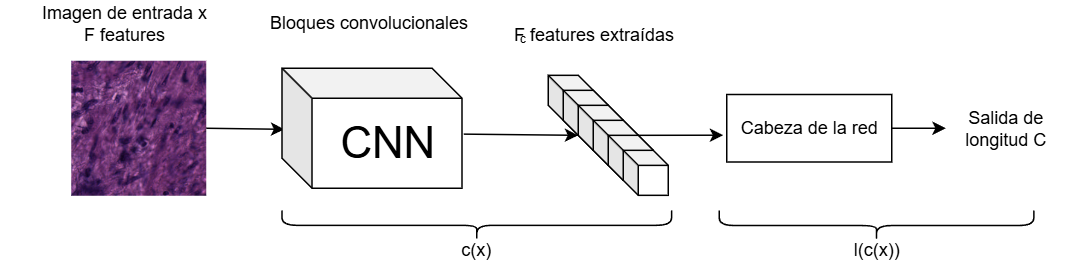
\includegraphics[scale=0.45]{images/fxshield_esquema}}
\caption{Esquema de la red completa. En este se diferencian las características extraídas por las capas convolucionales de la red de las características de la entrada.}
\label{fig:fxshield_esquema}
\end{figure}


Para X-SHIELD las características de las entradas, si son imágenes, dependen de como se quieran definir. Hay varias posibilidades como tomar que cada píxel se corresponda a una características, dividir la imagen en de entrada en cuadrados del mismo tamaño o utilizar métodos para dividir la imagen de entrada en superpíxeles. En FX-SHIELD la toma de esta decisión no es necesaria porque independientemente de la imagen de entrada (incluso para distintos tamaños de esta) siempre se va a obtener el mismo número $F_c$ de características extraídas por los bloques convolucionales. 

Notemos como $z=c(x)$ las características intermedias. Ahora buscamos ocluir las características menos importantes de $z$. La importancia que se le da a las distintas características se puede definir con la matriz de importancia $\mathcal{A} = \frac{\delta f}{\delta Z}(x) = \frac{\delta l}{\delta Z}(z)$. Para cada características $i \in \{1,2,...,F_c\}$ vamos a definir la importancia de esta como:

\begin{equation}
I_i(z) =  \frac{||\mathcal{A}_i||_1}{C} = \frac{1}{C}\sum_{j=1}^C |\mathcal{A}_{i,j}| 
\end{equation}

Por lo tanto esta es la media aritmética de la suma absoluta de la derivada de cada valor de salida sobre dicha características. Volviendo al ejemplo de la arquitectura de EfficientNet-B2 \ref{tab:EfficientNetB2_arquitectura} tenemos que la cabeza de la red consta de una única capa totalmente conectada, es decir en este caso se tiene que:

\begin{equation}
l(z) = Az + B
\end{equation}

Dónde $A$ es una matriz real de dimensión $C\times F_c$ y $B$ es un vector de $C$ valores. Como $l$ es una aplicación lineal se sigue que $\mathcal{A}=A$ y la importancia no es más que la suma para cada característica de los valores de $A$ para esta.

Sea $\lambda\in [0,100]$ un parámetro que determina que porcentaje de las características se va a ocultar, definimos la siguiente transformación $T_{fxshield}: \mathbb{R}^{F_c} \rightarrow \mathbb{R}^{F_c}$ que enmascara el $\lambda \%$ de elementos menos importantes. En la práctica se escoge el menor $m$ tal que $\lambda < \frac{m}{F_c} \cdot 100$ y se enmascaran las $m$ características menos importantes. En X-SHIELD, como se enmascaran características de la entrada que son imágenes, lo que se hace es sustituir estas por el color medio de la entrada. Para FX-SHIELD estamos en el espacio de features, dónde los valores que van de $-\infty$ a $\infty$. Por lo tanto hemos decidido sustituir dichos valores por $0$. Suponiendo, sin pérdida de generalidad, que las características en $z$ están ordenadas de menor importancia a mayor, se define $T_{fxshield}$ como:

\begin{equation}
z' = T_{fxshield}(z) = (0,0,...,0,z_{m+1},...,z_{F_c})
\end{equation}

Ahora podemos medir la predicción del modelo para este ejemplo modificado simplemente pasándolo por la cabeza de la red. 

Ya estamos en condiciones de definir el factor de regularización que se utiliza en este método. Para un ejemplo $x$ y unos parámetros $\Theta$ del modelo específicos, sean $y=f_\Theta(x)=l(z)$ la predicción original del modelo y $y'=l(T_{fxshield}(c_\Theta(x))) = l_\Theta(z')$ la predicción para el ejemplo con las características intermedias modificadas, entonces se tiene que:

\begin{equation}
FX-SHIELD(x,\Theta) = KL(y,y') + KL(y',y)
\end{equation}

Dónde $KL$ es la divergencia de Kullback-Leibler que se utiliza para medir la distancia estadística entre las distribuciones de probabilidad entre los modelos.

Es decir, FX-SHIELD utiliza este valor regularizador en el entrenamiento por lo que en este método se minimiza la siguiente función:

\begin{equation}
coste\_fxshield(\Theta,X,Y) = funcion\_perdida(f_\Theta(X),Y) + FX-SHIELD(X,\Theta)
\end{equation}


Una ventaja que presenta este método sobre X-SHIELD es que no necesita que el modelo de caja negra sea diferenciable, aunque sigue necesitando que la cabeza del modelo lo sea (para el cálculo de la importancia de las características). A cambio, FX-SHIELD no es totalmente agnóstico al modelo, pues es necesario poder extraer unas características intermedias.

Otra ventaja es que es más rápido que X-SHIELD ya que para el cálculo de la regularización no hace falta pasar las características enmascaradas por toda la red sino por las capas posteriores a las convolucionales, que suelen ser mucho más rápidas y con menos parámetros.

En X-SHIELD se esconden las características menos relevantes de la entrada a la red, que es una imagen, con la idea de eliminar partes de imagen que no son relevantes para la tarea de clasificación. En FX-SHIELD se esconden las características menos relevantes de las extraídas por las capas convolucionales. Esto puede ser interesante pues varios trabajos anteriores como \cite{NetDiss,tcav,distill} muestran que las capas intermedias en CNNs representan conceptos de alto nivel. Por lo tanto tiene sentido trabajar con estas características intermedias que codifican conceptos que tienen sentido para los humanos. Esto se puede ver como una ventaja de FXSHIELD sobre X-SHIELD (cuando se toman características de la imagen de entrada como una división de la imagen en cuadrados) ya que estas features intermedias pueden tener un mayor significado.

\subsection{FRShield}

\textbf{FRSHIELD} (\textit{Random FX-SHIELD}) es el mismo método que FX-SHIELD pero cambia en que las características que oculta se escogen de forma aleatoria sin tener en cuenta la importancia de estas. Este método nos permite comparar FX-SHIELD con un método no informado. Además el hecho de que se oculten las características de forma aleatoria puede ayudar al modelo a no depender únicamente de las características más importantes y que las explicaciones estén apoyadas en más características. Finalmente este método se parece a \textit{Dropout}, lo que también lleva a pensar que podría hacer que la red no sobreentrene.

\subsection{HShield}

Finalmente introducimos \textbf{H-SHIELD} (\textit{Hybrid} X-SHIELD) un método que combina X-SHIELD con FX-SHIELD. Para ello modificamos el valor regulador para tener en cuenta ambos de la siguiente forma:

\begin{align*}
coste\_hshield(\Theta,X,Y) = &funcion\_perdida(f_\Theta(X),Y) + \\
&\alpha_1 \cdot X-SHIELD(X,\Theta) +\\
&\alpha_2 \cdot FX-SHIELD(X,\Theta)
\end{align*}

Dónde $\alpha_1, \alpha_2$ son dos parámetros positivos que utilizaremos para darle cambiar el peso que le damos a cada una de las regularizaciones por separado. 

Con esta propuesta intentamos combinar las bondades de ambos métodos. El principal inconveniente de este método es su mayor coste computacional a los métodos por separado. La determinación de los parámetros $\alpha_1$ y $\alpha_2$ se hará empíricamente comparando los valores de regularización individuales que se obtienen para cada método por separado. El porcentaje de elementos que se ocultan por cada método, que denotabamos como $\lambda$, ahora son dos parámetros distintos $\lambda_1$ y $\lambda_2$, que serán dicho parámetro para X-SHIELD y FX-SHIELD respectivamente.

\section{Implementación}

Para la realización de este TFM se ha partido del \href{https://github.com/isega24/SHIELD/tree/X-SHIELD}{código} correspondiente al proyecto de X-SHIELD original \cite{XSHIELD}. Este está escrito en \textit{Python}. Se ha realizado un estudio de todo el código de el proyecto original para entender correctamente como funciona y así poder implementar los nuevos métodos que proponemos. Además se han escrito varios \textit{scripts} en \textit{bash} para la ejecución de los entrenamientos de los modelos aplicando los distintos métodos de regularización  en los servidores de GPUs de la UGR.

A continuación hacemos un resumen de todos los módulos del proyecto que se han utilizado, sin contar los \textit{scripts} de \textit{bash} de , y mencionamos cuando se han modificado para el TFM:

\begin{itemize}
\item \textbf{SHIELD/shield.py:} este es el módulo más importante de todo. En él vienen las funciones para calcular las importancias de las características y las implementaciones de los distintos métodos. En particular se ha añadido a este archivo los métodos X-SHIELD y R-SHIELD.

\item \textbf{procedures/cargar\_datos.py:} este módulo es completamente nuevo y es necesario para cargar los datos del TFM en un \textit{dataset} de \textit{pytorch}. Este módulo se basa en la manera en la que se cargan los \textit{datasets} utilizados en el trabajo original de X-SHIELD, cuya implmentación se puede ver en el \href{https://github.com/ari-dasci/S-ReVel}{GitHub} de las métricas REVEL.

\item \textbf{procedures/procedures.py:} aquí vienen implementadas las funciones para cargar el modelo clasificador (\textit{EfficientNet} en nuestro caso) y las funciones que realizan un paso en entrenamiento y validación.

\item \textbf{tests/test.py y tests/train.py:} scripts para el entrenamiento de la red con X-SHIELD y para obtención de \textit{accuracy} en test, respectivamente.

\item \textbf{tests/mitrain.py, tests/mitest.py, tests/mitrain\_hibrido.py:} los dos primeros son scripts para el entrenamiento de la red con X-SHIELD o FX-SHIELD y para obtención de \textit{accuracy} en test, respectivamente. El tercero es una adaptación para entrenar H-SHIELD. Estos son muy parecidos a los anteriores pero están adaptados para utilizar nuestro conjunto de datos y los nuevos métodos.

\item \textbf{tests/REVEL\_metrics.py y tests/mi\_REVEL\_metrics.py:} \textit{script} original para calcular las métricas REVEL para un modelo y la versión modificada para utilizar el conjunto de datos de este TFM.
\end{itemize}

Además durante la ejecución de los experimentos se disponía de una carpeta llamada \textbf{datosTFM} dónde había dos carpetas, \textbf{train} y \textbf{val} que contenían los datos de entrenamiento y test respectivamente.

Para la gestión de paquetes de \textit{Python} se ha utilizado la herramienta \textit{Conda} que permite crearentornos con los paquetes de \textit{Python} necesarios para el proyecto. Se ha utilizado la versión de Conda 4.10.1 y se ha creado un entorno con Python 3.9.23. Se han instalado los siguiente paquetes paquetes de \textit{Python}:

\begin{itemize}
    \item torch (versión 2.0.1): con CUDA versión 11.7
    \item torchvision
    \item tensorboard
    \item efficientnet\_pytorch
    \item torchsummary
    \item numpy
    \item pandas
    \item scipy
    \item scikit-learn
    \item scikit-image
    \item matplotlib
    \item seaborn
    \item plotly
    \item tqdm
    \item opencv-python
    \item ipywidgets
    \item ipython
    \item wget
    \item captum
    \item revel-xai: paquete con la implementación de las métricas REVEL.
\end{itemize}

Todo el código desarrollado para el TFM está disponible en el siguiente \href{https://github.com/CarlosLaraCasanova/Codigo_TFM/tree/main}{enlace}.


\clearpage


\newpage
\chapter{Experimentos} \label{cap:exp}



\section{Datos empleados} \label{sec:datos}

El conjunto de datos empleado está desarrollado por la iniciativa \textit{aI4HealthyAging}. En particular se creó para el paquete de trabajo 7: cribado y vigilancia activa en cánceres prevalente de la 3ª edad.

\highlight{LA CITA BIBLIOGRÁFICA SIGUIENTE (\cite{datosObtencion} la he creado yo. Se corresponde al archivo que  me mandaste con información del dataset, pero no he podido encontrarlo online.} 

\paragraph*{Metodología de obtención y etiquetado de imágenes}

Para la obtención de las imágenes siguieron la metodología que se puede consultar en \cite{datosObtencion}. En esta siguen el procedimiento estándar de procesamiento hispatológico. Partían de muestras de prostatectomía radical (la extirpación completa de la próstata). A continuación la fijan en formalina. Tras esto un patólogo o residente de patología realiza un examen macróscopico para extraer muestras para estudiar con microscopio. Estas muestras de tejido se procesan deshidratándolos e impregnándolos en parafina. Luego se cortan secciones del tejido de entre 3 $\mu m$ y 5 $\mu m$. Después se colocan en láminas de vidrio y se tiñen con hemaxtoxilina-ecosina. Finalmente se cubren con otra lámina de vidrio para ser examinados con un microscopio.

A continuación las muestras se escanearon en un escáner de láminas, lo que produjo imágenes en formato \textit{TIFF}. Dichas imágenes fueron segmentadas manualmente por patólogos profesionales del servicio de anatomía patológica del Hospital Miguel Servet de Zaragoza (ver Figura \ref{fig:datoSegmentado}). Los diferentes segmentos fueron anotados como pertenecientes a una de las 14 clases posibles, presentes en la Tabla \ref{tab:datasetClases}. Para llevar a cabo el etiquetado hicieron uso de la plataforma \textit{Cytomine}. 


Finalmente las imágenes se fragmentan en parches de tamaño $224\times 224$ píxeles. Cuando cuando un parche contiene una proporción de píxeles perteneciente a una clase superando el umbral $h = 0.75$ este parche se anota con dicha clase, si esto no ocurre para ninguna clase se descarta el parche. 

Esta es la versión del conjunto de datos con el que partimos nosotros, tenemos los parches que han sido anotados con una de las 14 clases.

\begin{longtable}{|p{4cm}|p{8cm}|p{3cm}|}

\hline
\textbf{Nombre} & \textbf{Descripción} & \textbf{Tipo} \\
\hline
\endfirsthead

\multicolumn{3}{c}%
{{\bfseries \tablename\ \thetable{} -- continuación}} \\
\hline
\textbf{Nombre} & \textbf{Descripción} & \textbf{Tipo} \\
\hline
\endhead

\hline \multicolumn{3}{r}{{Continúa en la siguiente página}} \\
\endfoot

\endlastfoot

Tejido sano diferente a estroma (HT) & Tejido sano sin estructuras relevantes asociadas a malignidad & Tejido no maligno \\
\hline
Estroma sano (HS) & Estroma sin estructuras relevantes asociadas a malignidad & Tejido no maligno \\
\hline
Glándulas no neoplásicas (NG) & Glándulas con morfología no neoplásica & Tejido no maligno \\
\hline
Tejido inflamatorio (IT) & Tejido con signos de inflamación &  Tejido no maligno \\
\hline
Gleason 3 (G3) & Glándulas individuales, bien formadas, de tamaño variable, separadas por estroma &  Tejido maligno \\
\hline
Gleason 4, patrón cribiforme (G4c) & Glándulas compuestas por células tumorales dispuestas en trabéculas redondeadas o irregulares, cohesivas, con perforaciones o luces perforadas &  Tejido maligno \\
\hline
Gleason 4, patrón glándulas fusionadas (G4f) & Glándulas sin estroma entre ellas, con luz glandular conservada & Tejido maligno \\
\hline
Gleason 4, patrón glándulas pobremente formadas (G4p) & Glándulas pequeñas con luces desproporcionadas & Tejido maligno \\
\hline
Gleason 4, patrón glomeruloide (G4g) & Glándulas con un nido de células tumorales que ocupa la luz y está unida a la glándula por un polo &  Tejido maligno \\
\hline
Gleason 5, patrón comedonecrosis (G5c) & Nidos tumorales redondeados con necrosis central de tipo comedo & Tejido maligno \\
\hline
Gleason 5, patrón sin glándulas definidas (G5w) & Células tumorales sueltas, en hilera o trabéculas. Ausencia de diferenciación glandular &  Tejido maligno \\
\hline
Neoplasia intraepitelial prostática de alto grado (PIN) & Glándulas con capa basal y proliferación de células epiteliales con atipia y pérdida de mucosecreción; patrones micropapilar, cribiforme, plano, hiperplásico & Tejido maligno \\
\hline
Adenocarcinoma ductal (DA) & Glándulas cribiformes y estructuras papilares y/o complejas revestidas por células altas columnares pseudoestratificadas & Tejido maligno \\
\hline
Carcinoma intraductal (IC) & Grandes ductos con capa basal y luz dilatada, distendida y ocupada por proliferación de células epiteliales con marcada atipia y crecimiento papilar, cribiforme laxo o cribiforme denso &  Tejido maligno \\
\hline

\caption{En esta tabla se muestra la clasificación de los tejidos, una breve descripción de qué significan y si el tejido es maligno. Tabla extraída y adaptada de \cite{datosObtencion}.} \label{tab:datasetClases} 
\end{longtable}


\begin{figure}[h]
\noindent
\makebox[\textwidth]{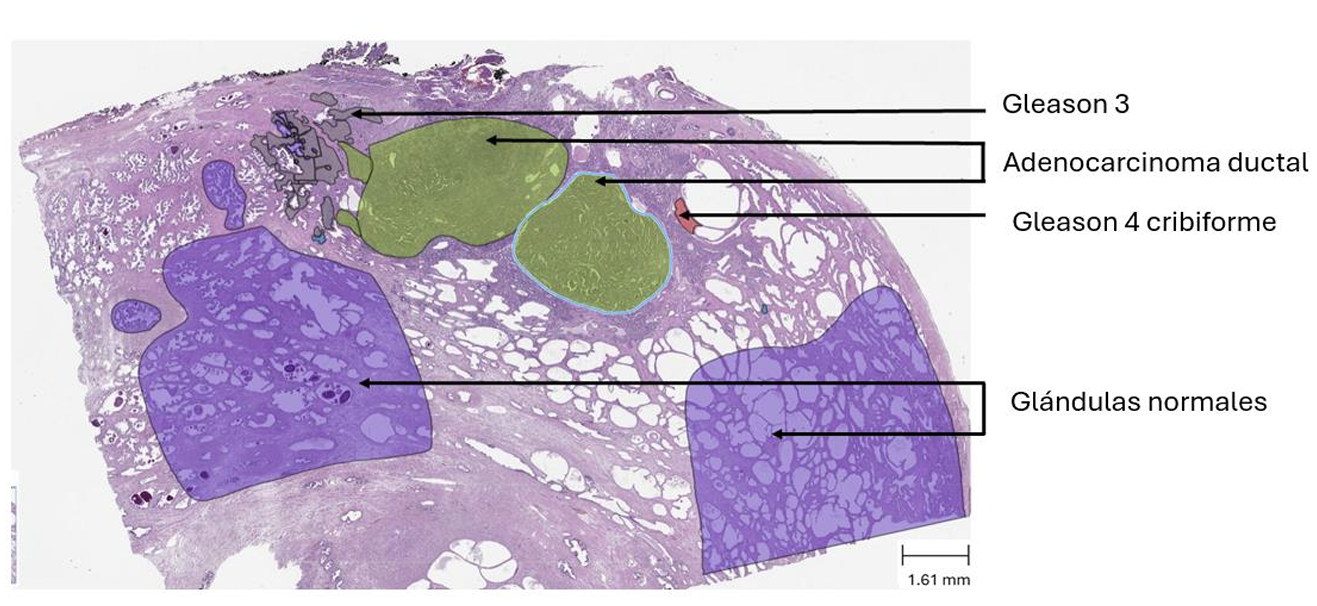
\includegraphics[scale=0.6]{images/datoSegmentado}}
\caption{Imagen de tejido segmentado. Imagen extraída de \cite{datosObtencion}.}
\label{fig:datoSegmentado}
\end{figure}

\paragraph*{Distribución de los datos}

En total, el conjunto de datos contiene 126.109 imágenes anotadas. La distribución de estos entre las distintas clases se muestra en la Figura \ref{fig:distribucionDatos}. Se puede apreciar un claro desbalanceo en los datos. La clase menos frequente es Gleason 4 glomeruloide (G4p) con 243 datos ($~0.19\%$ de los datos), mientras que la más frecuente es Glándulas no neoplásticas (NG) con 35.894 datos ($~28.46\%$ de los datos). 


\begin{figure}[h]
\noindent
\makebox[\textwidth]{\includegraphics[scale=0.6]{images/distribucionDatos}}
\caption{Distribución de las imágenes del conjunto de datos según su clase.}
\label{fig:distribucionDatos}
\end{figure}


Además los datos están divididos en dos carpetas \textit{train} y \textit{val}. La carpeta \textit{train} contiene 113.491 imágenes ($~90\%$ de los datos) mientras que \textit{val} contiene las 12.618 imágenes restantes ($~10\%$ de los datos). Está partición de los datos se realizó para entrenamiento/test de los modelos y vamos a respetarla. Se puede comprobar que esta partición de los datos mantiene la proporción de las clases como se puede ver en la Figura \ref{fig:distribucionDatosTrainTest}.


\begin{figure}[h!]
\noindent
\makebox[\textwidth]{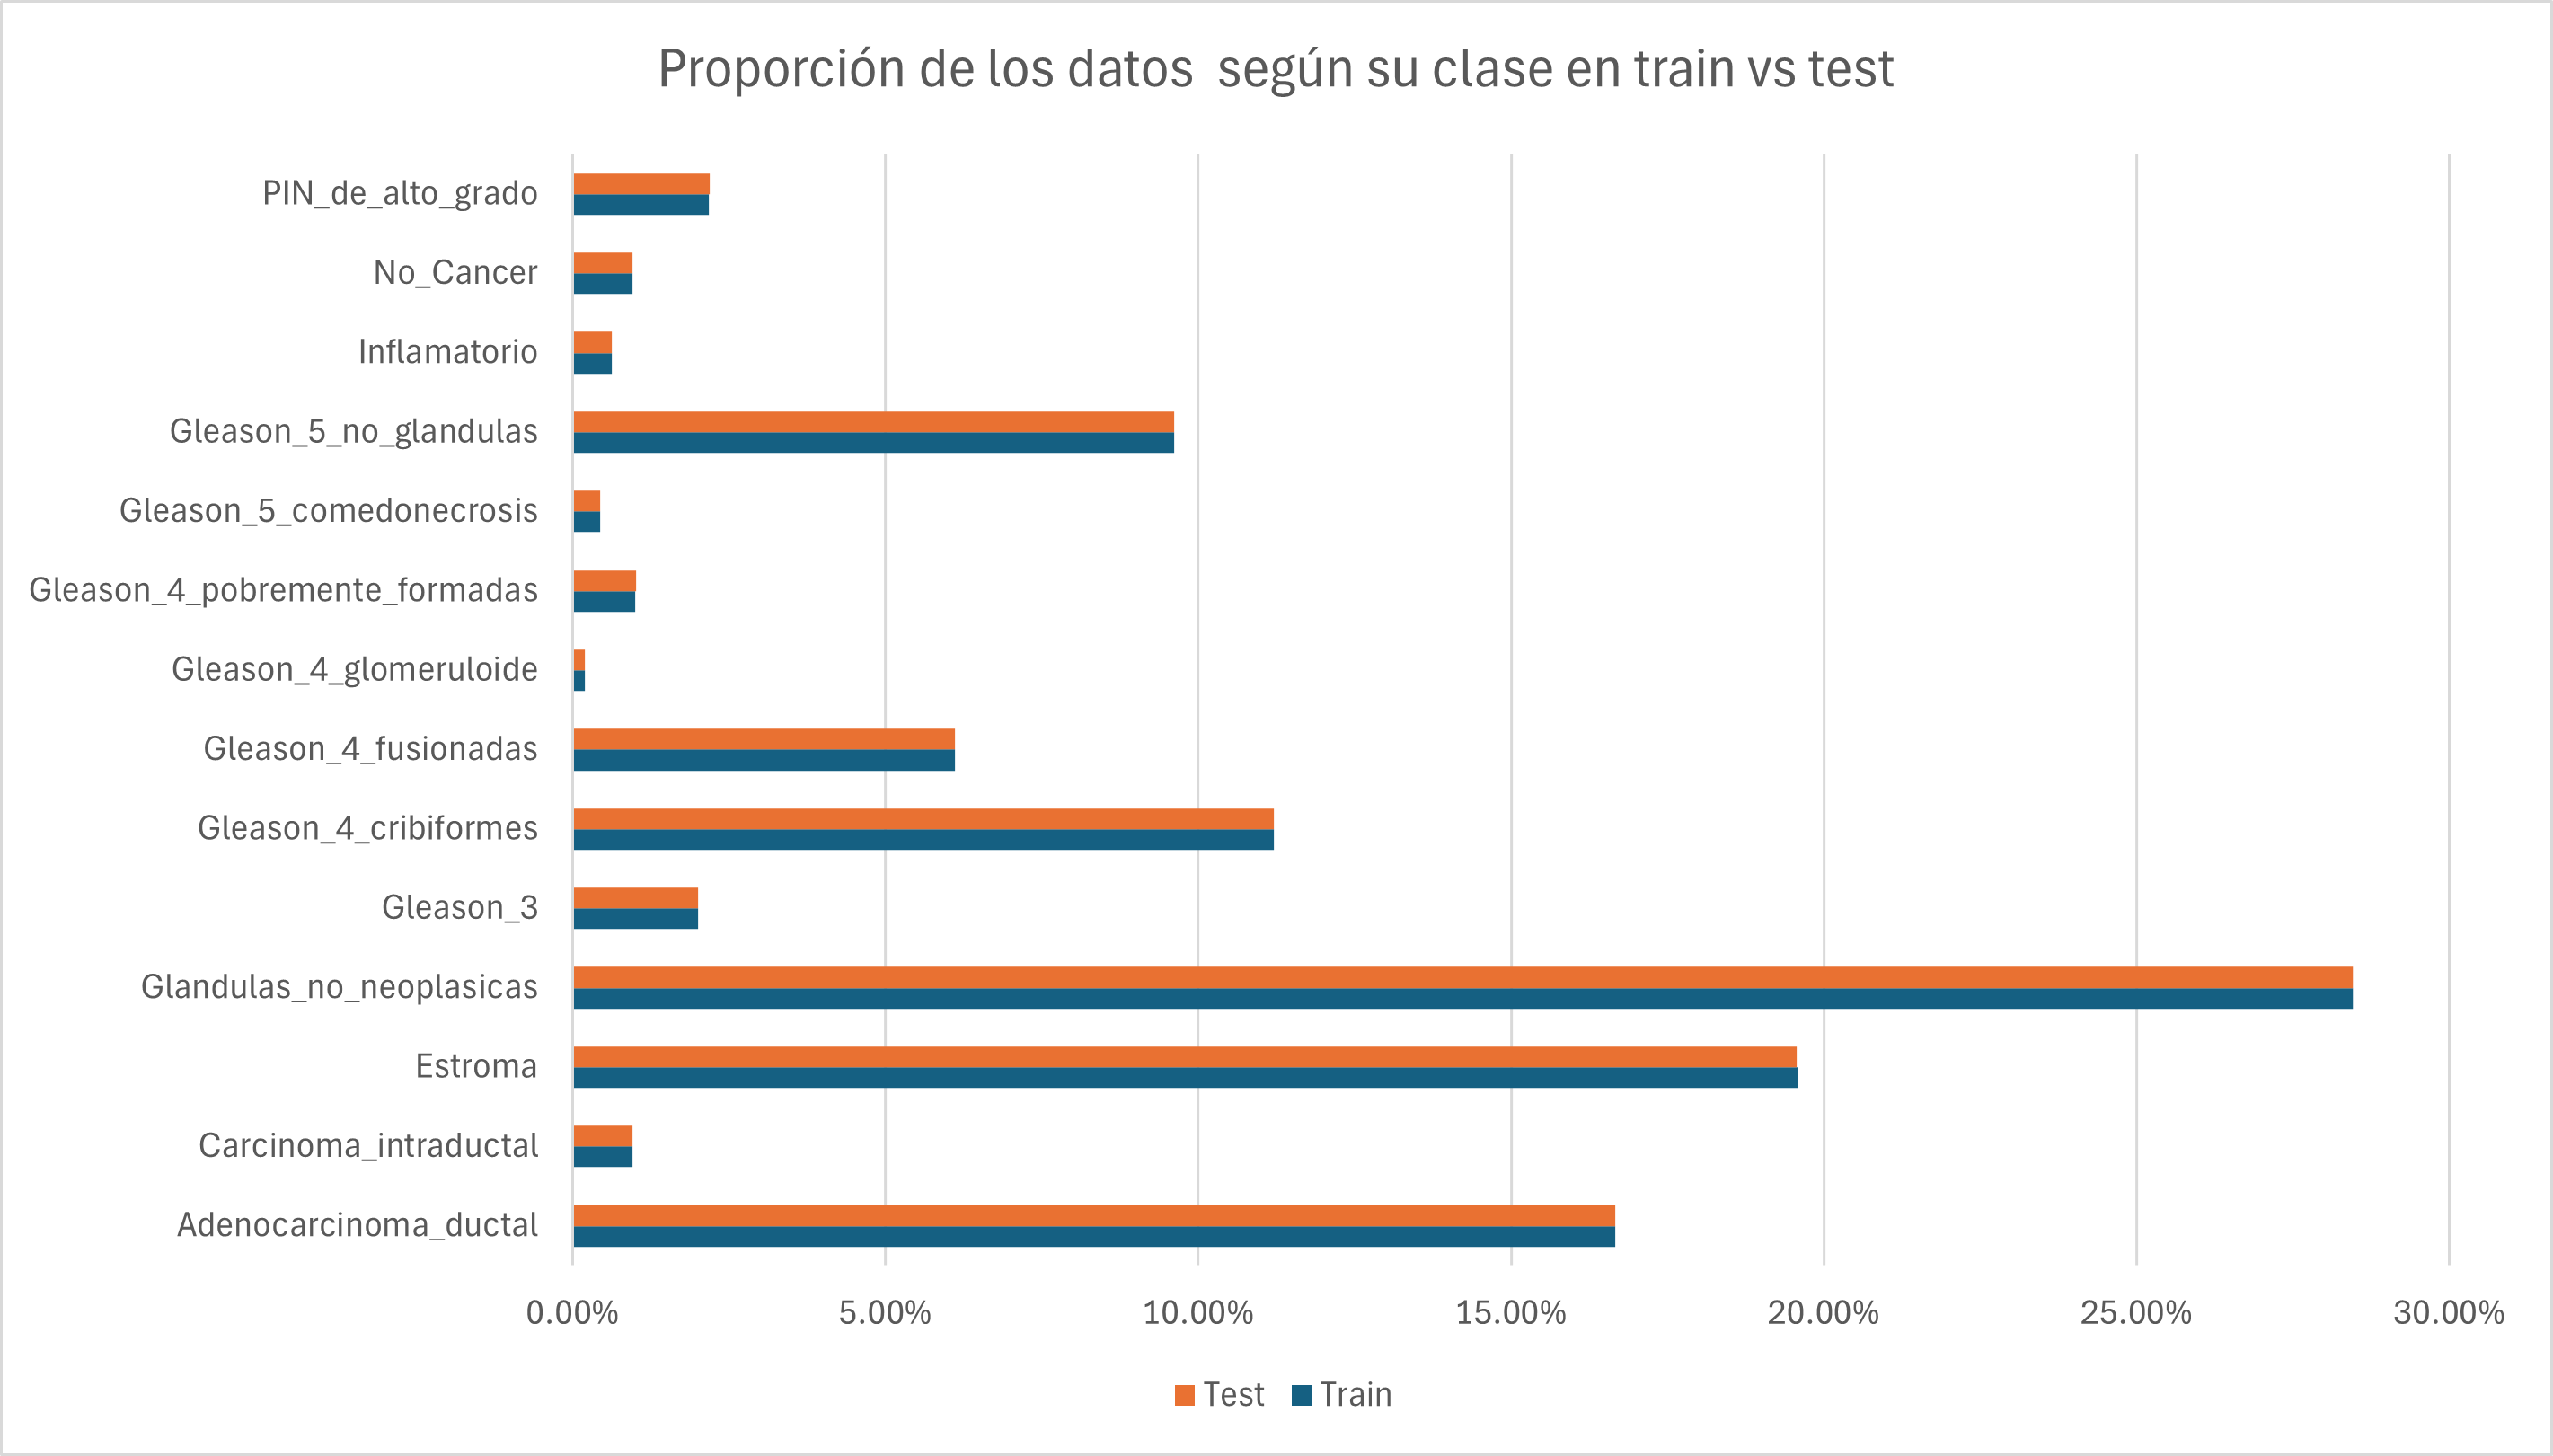
\includegraphics[scale=0.6]{images/DatosProporcionTestTrain}}
\caption{Distribución de las imágenes del conjunto de datos para entrenamiento y para test según su clase.}
\label{fig:distribucionDatosTrainTest}
\end{figure}



\section{Experimentos realizados}

Los experimentos han sido ejecutados en los servidores de cómputo Atenea y Hera, de los servidores NGPU de la Universidad de Granada. Las gráficas utilizadas son GTX Titan Xp con 128 Gb DDR4 y Titan RTX con 128 Gb DDR4, respectivamente.

\subsection{Separación de datos}

Cómo ya hemos comentado realizamos una división 90/10 de los datos totales entre entrenamiento/test. Los modelos se van a entrenar con el conjunto de entrenamiento y se evaluará con los datos del conjunto de test. Esta división de los datos se realiza para tener un conjunto,
el de test, que no haya visto el modelo durante el entrenamiento para evaluar el rendimiento
real del modelo para datos que aún no ha visto. Esta práctica es muy importante para evitar
el sobreentrenamiento de la red. La división de 90/10 de los datos tiene sentido sobre otras típicas como 80/20 porque disponemos de una cantidad muy grande de datos (126.109 imágenes).

\paragraph*{Validacion}

Teniendo en cuenta el tamaño de nuestro conjunto de datos y de los recursos computacionales de los que disponemos hemos decidido utilizar un conjunto de validación fijo sobre otros métodos como \textit{k-fold cross validation}. 


Esta técnica consiste en separa un porcentaje del conjunto de entrenamiento para no entrenar con él. Sin embargo se va a utilizar para evaluar el modelo al final de cada época, calculando su función de error sobre este conjunto. Esta técnica es importante para el entrenamiento del modelo porque que cumple un rol distinto a los conjuntos de entrenamiento y test. Este nos ayudará a realizar un ajuste de hiperparámetros del modelo y ayuda a prevenir el sobreajuste, eligiendo el modelo que menor error tenga en validación, en vez de en entrenamiento. 

Nosotros vamos a dividir el conjunto de entrenamiento en 90/10 para entrenamiento y para validación respectivamente. En la Figura \ref{fig:distribucionTrainTestVal} presentamos un esquema con la división del conjunto de datos seguida para los experimentos.


\begin{figure}[h!]
\noindent
\makebox[\textwidth]{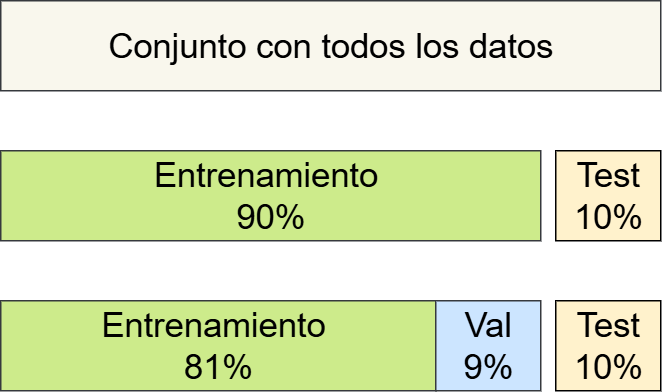
\includegraphics[scale=0.4]{images/divisionDatos}}
\caption{Distribución de los datos en los conjuntos finales de entrenamiento, validación y test.}
\label{fig:distribucionTrainTestVal}
\end{figure}

\subsection{Elección de hiperparámetros}


El \textbf{optimizador} elegido para entrenar el modelo es Adam \cite{adam}, que es una modificación de SGD. Se ha elegido este optimizador porque es el que se utilizó originalmente en el artículo de X-SHIELD \cite{XSHIELD} y porque está probado empíricamente que tiene mejor rendimiento que el resto de optimizadores para una gran variedad de tareas.

Cómo \textbf{\textit{learning rate}} inicial Adam se ha escogido el valor $0.0004$. Un \textit{learning rate} inicial es muy importante porque dicta como converge el modelo. Para la elección de este parámetro se han hecho pruebas iniciales sobre los modelos y hemos determinado que este valor es el que mejor convergencia daba al modelo.

El tamaño del \textbf{\textit{minibatch}} escogido ha sido 32. Está demostrado que tamaños grandes de \textit{minibatches} acelera el entrenamiento y estabiliza la convergencia del modelo. Por otro lado un tamaño pequeño puede mejorar la capaz de generalizar del modelo \cite{batchSize}. El tamaño suele escogerse como una potencia de $2$. Hemos escogido tamaño $32$ ya que para $64$ la gráfica dónde ejecutamos los experimentos se quedaba sin memoria y empíricamente se comprobó que $32$ daba mejores resultados que tamaños menores.

Para el número de \textbf{épocas} hemos escogido un número no muy alto ya por los recursos computacionales de los que disponemos. Por ello se hicieron pruebas experimentales previas para buscar un valor que garantizaba la convergencia de estos pero no se excedía en tiempo de entrenamiento. El número de épocas es por lo tanto $24$. Con este número de épocas los modelos entrenados con la regularización X-SHIELD (la más costosa) tardan alrededor de 1 día (normalmente un poco más) en entrenarse.

Cómo ya sabemos el modelo que vamos a utilizar en los experimentos es EfficientNet-B2 con entradas de tamaño $224 \times 224$. Este modelo lo cargamos de la librería de \textit{pytorch}. Además lo vamos a cargar con los pesos preentrenados de esta red sobre el conjunto de datos IMAGENET-1K lo que se conoce como \textit{transfer learning} y nos permite no tener que entrenar el modelo desde cero.

En primer lugar vamos a entrenar el modelo EfficientNet-B2 base con los parámetros que hemos especificado. Después se entrenará esta red aplicando los distintos métodos de regularización explicados, estos son: el método original con el que comparamos los propuestos (X-SHIELD) y los métodos nuevos que proponemos en este trabajo (FX-SHIELD, FR-SHIELD y H-SHIELD).

Los hiperparámetros a los que se va a probar a cambiar sus valores son los correspondientes a los métodos de regularización de XAI. Estos son:

\begin{itemize}

\item $\lambda$: En el caso de X-SHIELD, FX-SHIELD y FR-SHIELD este parámetro determina que porcentaje de las caracterísitcas (de las entrada en el caso de X-SHIELD y los intermedios en el caso de los nuestros) se van a ocultar para el cálculo de los valores de regularización. Para X-SHIELD se ha probado con los parámetros 3, 6, 9 y 12, ya que en \cite{XSHIELD} se demostró que funcionaba mejor para valores similares a estos. Para los métodos nuevos, como no tenemos esta información hemos probado con más variedad de valores. Para FX-SHIELD hemos probado con los parámetros a 3, 6, 9, 12, 25, 35, 45, 55, 65, 75 y 85, como funcionaba mejor para 75 también probamos con los valores vecinos 70, 73 y 77. Para FR-SHIELD hemos probado con 3, 45, 65, 75 y 77.

\item $\alpha_1$ y $ \alpha_2$: Estos son los parámetros para H-SHIELD. Son los pesos que se aplican a la regularización X-SHIELD y FX-SHIELD respectivamente. Para los hiperparámetros $\lambda$ para cada uno de estos hemos escogido los que mejores resultados daban por individual que son 12 y 77 respectivamente. Para $(\alpha_1,\alpha_2)$ se han probado $(1,1)$, $(1,2)$ y $(1,3)$
\end{itemize}

Además para las características de X-SHIELD se divide la imagen de entrada en 64 cuadrados del mismo tamaño para cada imagen como se hace en \cite{XSHIELD}.

De esta manera, el modelo se entrena aplicando cada método con la distintas elecciones de hiperparámetros. Para evitar el sobreentrenamiento, durante el entrenamiento de los modelos en cada época se calcula la función de pérdida sobre el conjunto de validación y el modelo final del entrenamiento es el que menor pérdida en validación haya obtenido, no necesariamente el que minimice el error en entrenamiento. 

Para elegir los mejores hiperparámetros para cada método se escoge modelo entrenado que minimicen la \textit{accuracy} en validación para dichos hiperparámetros.


\section{Métricas}

Para el entrenamiento del modelo se utiliza como función de pérdida el \textbf{error de entropía cruzada} que es la función de pérdida que se utiliza habitualmente para entrenar redes en clasificación.

Para evaluar el rendimiento del modelo en la tarea de clasificación utilizamos la \textbf{\textit{accuracy}} que mide la proporción de ejemplos correctamente clasificados. Esta toma valores en $[0,1]$ y cuanto mayor es, mejor es el rendimiento del modelo. 

Por otro lado para evaluar el rendimiento utilizamos la métricas \textbf{REVEL}. Estas fueron formalmente introducidas en \ref{subsec:revel}. Recordamos que estas son: \textit{local concordance}, \textit{local fidelity}, \textit{presciptivity}, \textit{conciseness} y \textit{robustness}. Para cada método de regularización las calcularemos únicamente para el modelo final que ha sido calculado para los mejores parámetros para dicho método.

Para el cálculo de estas métricas se deben crear explicaciones con un LLE. Elegimos \textbf{LIME}. Utilizamos las mismas características que X-SHIELD para LIME, es decir 64 cuadrados del mismo tamaño sobre la imagen de entrada.  Para los cálculos de la explicación de un ejemplo generamos 1000 vecinos. El parámetro $\sigma$ (explicado en la subsección \ref{subsec:LIME}) lo ponemos a 12.

Para cada ejemplo generamos 10 explicaciones para el cálculo de las cuatro primeras métricas y calculamos la media aritmética de cada una para obtener su valor final para ese ejemplo. En total utilizamos 100 ejemplos. Para el cálculo de la \textit{robustness} utilizan las 10 explicaciones generadas para las otras métricas para calcular esta métrica. Hemos elegido estos parámetros para calcular estas métricas por límites de coste computacional. El cálculo de estas métricas para un modelo ya entrenado tarda alrededor de 1 día.


\paragraph*{Test estadísticos bayesianos}

Una vez tenemos los 100 valores de las métricas REVEL para cada método utilizamos la librería de \textit{Python} \href{https://baycomp.readthedocs.io/en/latest/\#baycomp}{baycomp}. Esta biblioteca introduce los tests bayesianos para comparación de método. Estos tests permiten comparar dos métodos de manera probabilística, estimando directamente la probabilidad de que uno sea mejor que otro, o que la diferencia entre ellos sea insignificante.

Los tests de baycomp se basan en la estimación de la distribución posterior de la diferencia de desempeño entre dos métodos. Se calculan las tres probabilidades siguientes:
\begin{itemize}

\item Método A es mejor que método B.
\item Método B es mejor que método A.
\item Diferencia es irrelevante (\textit{Region of Practical Equivalence}, ROPE)

\end{itemize}

ROPE define un umbral de diferencia prácticamente insignificante. En la página del propio método recomienda ROPE = 0.01 para métricas en el rango $[0,1]$ que es el caso de las métricas REVEL (técnicamente \textit{robustness} podría ser negativa, en la práctica suele estar en el rango).

Diremos que un método es mejor que otro para una métrica cuando la probabilidad de que sea mejor es $>95\%$. Además de los test mostraremos las gráficas de violin para las distintas métricas y métodos. En particular compararemos: FX-SHIELD con X-SHIELD, porque X-SHIELD es un método probado que mejora el rendimiento de las métricas REVEL, FX-SHIELD con FR-SHIELD, para ver como influye ocluir características aleatorias y FX-SHIELD con HSHIELD, para ver como se comparan estos dos métodos nuevos.

\section{Resultados}

\subsection{Entrenamiento y accuracy}

Los resultados de todas las redes entrenadas con los distintos métodos y para todas las combinaciones de hiperparámetros se encuentran en la Tabla \ref{tab:resultadosTodo}. En esta se puede ver que hiperparámetros son los mejores para cada modelo, es decir, con qué parámetros han conseguido la mejor \textit{accuracy} en el conjunto de validación. Es destacable que para FX-SHIELD se obtiene el mejor resultado para $\lambda = 77$ mientras que para FR-SHIELD alcanza su mejor rendimiento con $\lambda = 3$. En H-SHIELD la mejor \textit{accuracy} se alcanza cuando se combinan X-SHIELD y FX-SHIELD con el mismo peso. Por otro lado X-SHIELD obtiene su mejor rendimiento con $\lambda = 12$ y es el que mejor \textit{accuracy} en validación obtiene de todos, aunque por un margen del $1\%$.



\begin{table}[htbp]
\centering
\arrayrulecolor{black} % color de las líneas
\setlength{\arrayrulewidth}{0.8pt} % grosor de las líneas
\begin{tabular}{|l|cccccc|}
\hline
\rowcolor{gray!50} Modelo & Train/Acc & Train/Loss & Train/Reg & Val/Acc & Val/Loss & Val/Reg \\
\hline
\textbf{Baseline} & \textbf{0.994} & \textbf{0.000600} & \textbf{0.0000} & \textbf{0.957} & \textbf{0.006017} & \textbf{0.0000} \\
\hline
\rowcolor{gray!10} X-SHIELD ($\lambda = 3.0$) & 0.985 & 0.001359 & 0.001278 & 0.958 & 0.004424 & 0.000167 \\
\rowcolor{gray!10} X-SHIELD ($\lambda = 6.0$) & 0.983 & 0.001570 & 0.001400 & 0.956 & 0.004638 & 0.000549 \\
\rowcolor{gray!10} X-SHIELD ($\lambda = 9.0$) & 0.980 & 0.001834 & 0.001541 & 0.954 & 0.004533 & 0.000660 \\
\rowcolor{gray!10} \textbf{X-SHIELD ($\lambda = 12.0$)} & \textbf{0.981} & \textbf{0.001751} & \textbf{0.001533} & \textbf{0.959} & \textbf{0.004191} & \textbf{0.001043} \\
\hline
\textbf{FR-SHIELD ($\lambda = 3.0$)} & \textbf{0.994} & \textbf{0.000572} & \textbf{0.000637} & \textbf{0.957} & \textbf{0.006000} & \textbf{0.000042} \\
FR-SHIELD ($\lambda = 45.0$) & 0.993 & 0.000636 & 0.004487 & 0.956 & 0.006579 & 0.002367 \\
FR-SHIELD ($\lambda = 65.0$) & 0.993 & 0.000682 & 0.018442 & 0.953 & 0.007386 & 0.011644 \\
FR-SHIELD ($\lambda = 75.0$) & 0.992 & 0.000754 & 0.046440 & 0.956 & 0.006569 & 0.030981 \\
FR-SHIELD ($\lambda = 77.0$) & 0.930 & 0.026030 & 0.011845 & 0.933 & 0.025997 & 0.011897 \\
\hline
\rowcolor{gray!10} FX-SHIELD ($\lambda = 3.0$) & 0.994 & 0.000592 & 0.000187 & 0.956 & 0.006643 & 0.000005 \\
\rowcolor{gray!10} FX-SHIELD ($\lambda = 6.0$) & 0.994 & 0.000570 & 0.000192 & 0.952 & 0.007051 & 0.000007 \\
\rowcolor{gray!10} FX-SHIELD ($\lambda = 9.0$) & 0.995 & 0.000531 & 0.000188 & 0.956 & 0.006387 & 0.000010 \\
\rowcolor{gray!10} FX-SHIELD ($\lambda = 12.0$) & 0.994 & 0.000599 & 0.000207 & 0.956 & 0.006427 & 0.000014 \\
\rowcolor{gray!10} FX-SHIELD ($\lambda = 25.0$) & 0.994 & 0.000594 & 0.000212 & 0.953 & 0.006608 & 0.000018 \\
\rowcolor{gray!10} FX-SHIELD ($\lambda = 35.0$) & 0.993 & 0.000608 & 0.000213 & 0.955 & 0.006220 & 0.000021 \\
\rowcolor{gray!10} FX-SHIELD ($\lambda = 45.0$) & 0.993 & 0.000687 & 0.000237 & 0.954 & 0.006806 & 0.000029 \\
\rowcolor{gray!10} FX-SHIELD ($\lambda = 55.0$) & 0.992 & 0.000718 & 0.000250 & 0.954 & 0.006480 & 0.000027 \\
\rowcolor{gray!10} FX-SHIELD ($\lambda = 65.0$) & 0.992 & 0.000759 & 0.000268 & 0.953 & 0.006728 & 0.000028 \\
\rowcolor{gray!10} FX-SHIELD ($\lambda = 70.0$) & 0.992 & 0.000784 & 0.000278 & 0.954 & 0.006237 & 0.000029 \\
\rowcolor{gray!10} FX-SHIELD ($\lambda = 73.0$) & 0.992 & 0.000741 & 0.000272 & 0.952 & 0.006556 & 0.000032 \\
\rowcolor{gray!10} FX-SHIELD ($\lambda = 75.0$) & 0.992 & 0.000786 & 0.000272 & 0.956 & 0.006146 & 0.000024 \\
\rowcolor{gray!10} \textbf{FX-SHIELD ($\lambda = 77.0$)} & \textbf{0.991} & \textbf{0.000833} & \textbf{0.000302} & \textbf{0.958} & \textbf{0.006351} & \textbf{0.000025} \\
\rowcolor{gray!10} FX-SHIELD ($\lambda = 85.0$) & 0.991 & 0.000883 & 0.000339 & 0.954 & 0.006527 & 0.000033 \\
\hline
\textbf{H-SHIELD ($\alpha_1=1.0, \alpha_2=1.0$)} & \textbf{0.973} & \textbf{0.002492} & \textbf{0.001862} & \textbf{0.954} & \textbf{0.072262} & \textbf{0.015705} \\
H-SHIELD ($\alpha_1=1.0, \alpha_2=2.0$) & 0.965 & 0.003278 & 0.002162 & 0.948 & 0.083916 & 0.015020 \\
H-SHIELD ($\alpha_1=1.0, \alpha_2=3.0$) & 0.953 & 0.004343 & 0.002547 & 0.948 & 0.083336 & 0.018308 \\
\hline


\end{tabular}
\caption{Resultados de entrenamiento y validación para diferentes métodos. Para cada método se muestran su error, valor de regularización y \textit{accuracy} en entrenamiento y validación. Para cada método se ha puesto en negrita el modelo que mejor \textit{accuracy} obtiene en validación que se considera el mejor modelo con dicho método.}
\label{tab:resultadosTodo}
\end{table}

\newpage
En la Tabla \ref{tab:resultadosMejoresTest} tenemos los valores obtenidos en test para los mejores modelos de cada método. Cómo esperábamos el método X-SHIELD mejora la \textit{accuracy} del modelo \textit{baseline}, en este caso en 0.07. Luego es una mejora significativa. Por otro lado el método híbrido H-SHIELD consigue capturar está mejoría, empeorando únicamente en un 0.01 su \textit{accuracy} respecto de X-SHIELD. Por otro lado los métodos FX-SHIELD y FR-SHIELD no han conseguido mejorar al modelo base, obteniendo ambas 0.949 de \textit{accuracy}, prácticamente la misma que el modelo base (un 0.01 de diferencia a favor del modelo base). Observemos también que H-SHIELD tiene con diferencia el mayor valor de su función de regularización en test a pesar de ser la suma de X-SHIELD y FX-SHIELD. Esto parece indicar que no es capaz de minimizar ambos valores de regularización al mismo tiempo.

\begin{table}[htbp]
\centering
\arrayrulecolor{black} % color de las líneas
\setlength{\arrayrulewidth}{0.8pt} % grosor de las líneas
\begin{tabular}{|l|ccc|}
\hline
\rowcolor{gray!50} Modelo & Test/Acc & Test/Loss & Test/Reg \\
\hline
Baseline & 0.950 & 0.005000 & 0.000 \\
X-SHIELD ($\lambda = 12.0$) & 0.957 & 0.004000 & 0.001 \\
FR-SHIELD ($\lambda = 3.0$) & 0.949 & 0.005000 & 0.000 \\
FX-SHIELD ($\lambda = 77.0$) & 0.949 & 0.005295 & 0.000064 \\
H-SHIELD ($\alpha_1=1.0, \alpha_2=1.0$) & 0.956 & 0.071610 & 0.015749 \\
\hline
\end{tabular}
\caption{Resultados de los mejores modelos en test. Se muestra la \textit{accuracy}, la pérdida y el valor de regularización.}
\label{tab:resultadosMejoresTest}
\end{table}


En la Figura \ref{fig:metrics_xshield} se encuentran las curvas de aprendizaje de X-SHIELD para sus distintos parámetros. Se observa un comportamiento natural de convergencia de la red, podría parecer que podría incluso mejorar un poco más viendo la gráfica del error en entrenamiento, aunque la de validación si parece que ha convergido. Es interesante ver que aunque en validación los valores de regularización siguen un orden y parecen converger a valores distintos (mayor cuanto mayor es el $\lambda$) lo cual es esperable, en entrenamiento estos convergen a valores muy cercanos.


% === Figura: xshield ===
\begin{figure}[H]
    \centering
    % Fila 1: Train (3 columnas)
    \begin{subfigure}[b]{0.3\textwidth}
        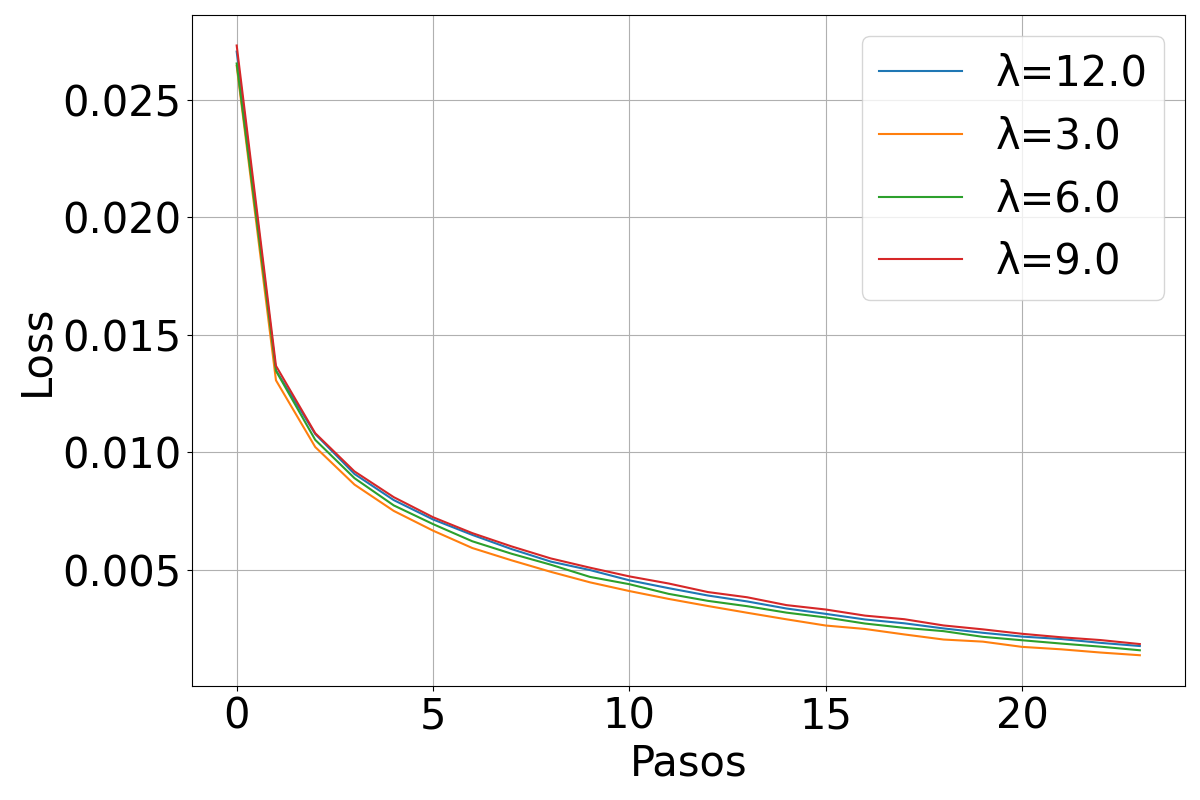
\includegraphics[width=\linewidth]{images/Train_Loss_evolucion_xshield.png}
        \caption{X-SHIELD - Train Loss}
    \end{subfigure}
    \hfill
    \begin{subfigure}[b]{0.3\textwidth}
        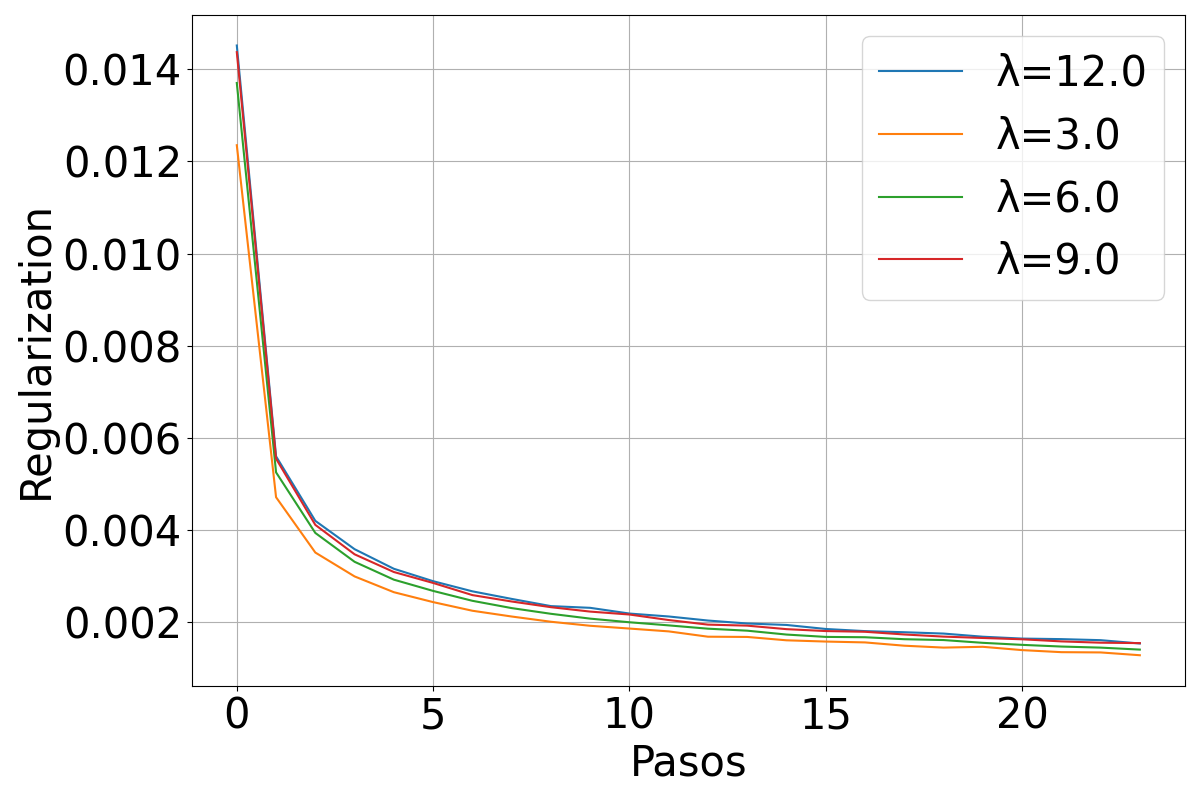
\includegraphics[width=\linewidth]{images/Train_Regularization_evolucion_xshield.png}
        \caption{X-SHIELD - Train Reg.}
    \end{subfigure}
    \hfill
    \begin{subfigure}[b]{0.3\textwidth}
        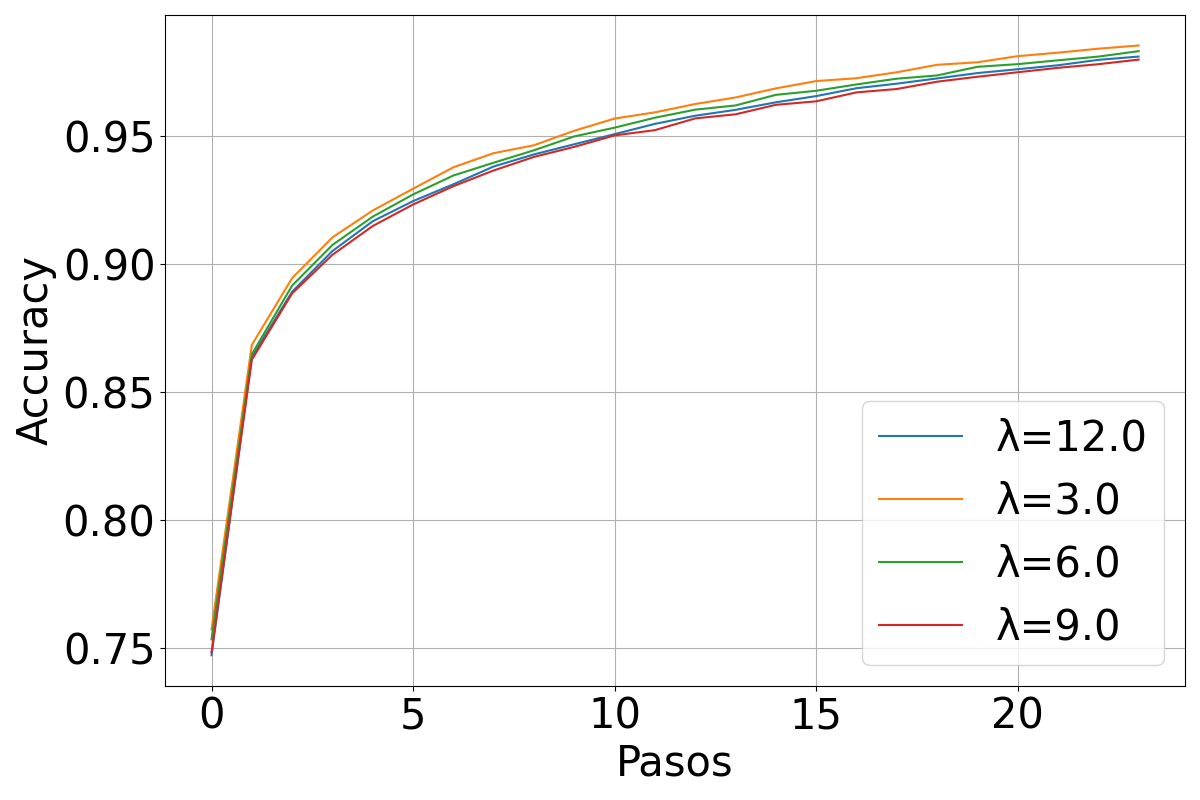
\includegraphics[width=\linewidth]{images/Train_Accuracy_evolucion_xshield.png}
        \caption{X-SHIELD - Train Acc.}
    \end{subfigure}

    \vspace{0.5em}

    % Fila 2: Val (3 columnas)
    \begin{subfigure}[b]{0.3\textwidth}
        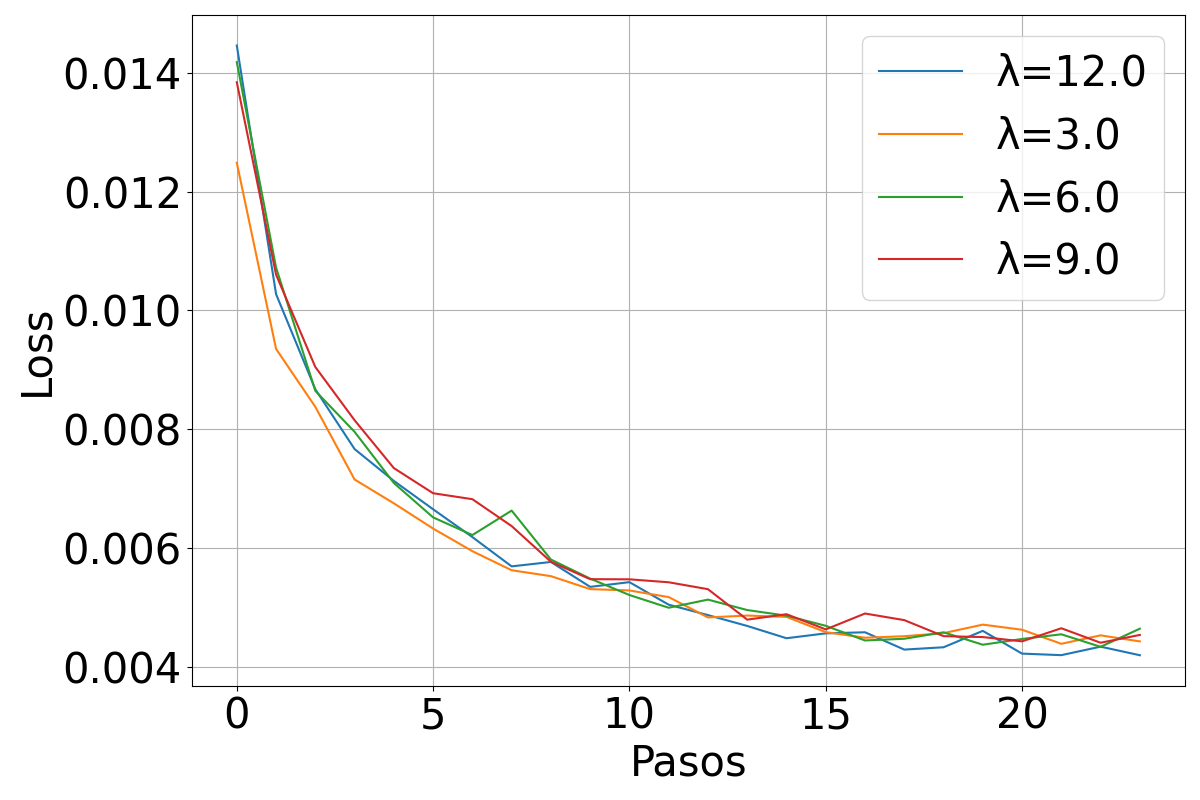
\includegraphics[width=\linewidth]{images/Val_Loss_evolucion_xshield.png}
        \caption{X-SHIELD - Val Loss}
    \end{subfigure}
    \hfill
    \begin{subfigure}[b]{0.3\textwidth}
        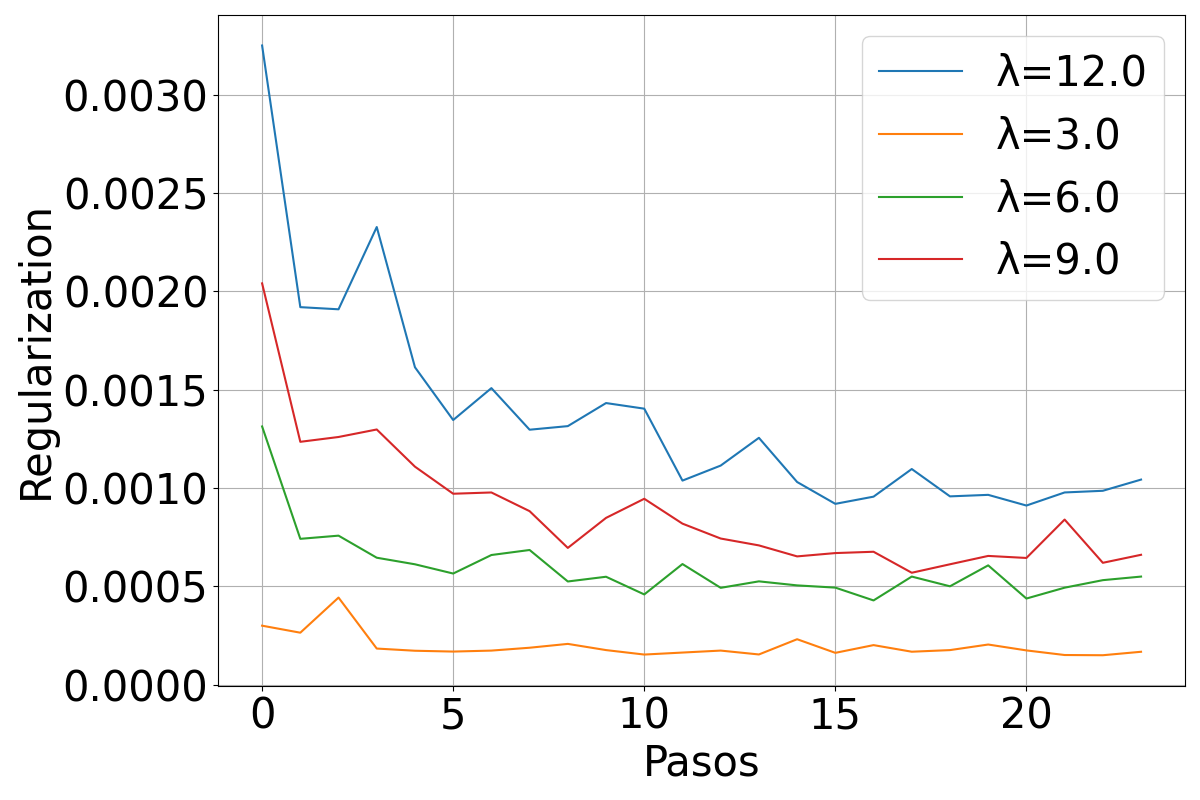
\includegraphics[width=\linewidth]{images/Val_Regularization_evolucion_xshield.png}
        \caption{X-SHIELD - Val Reg.}
    \end{subfigure}
    \hfill
    \begin{subfigure}[b]{0.3\textwidth}
        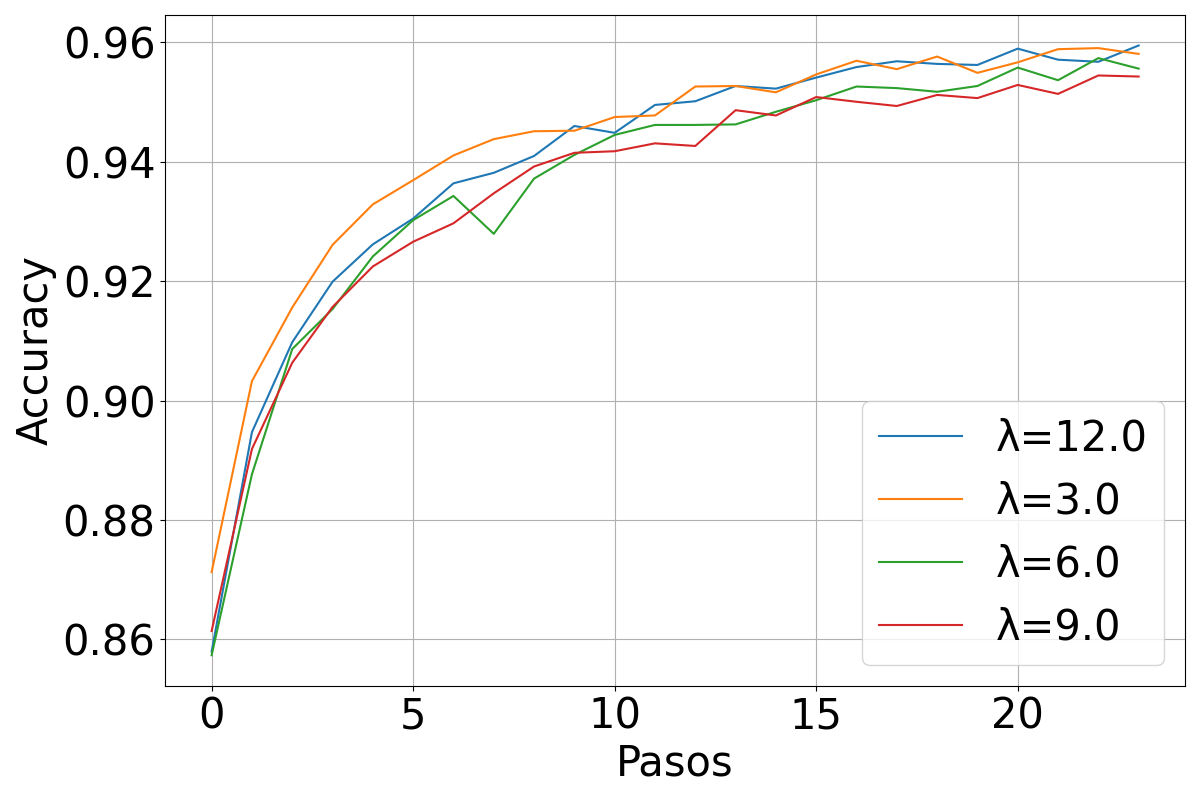
\includegraphics[width=\linewidth]{images/Val_Accuracy_evolucion_xshield.png}
        \caption{X-SHIELD - Val Acc.}
    \end{subfigure}

    \caption{Evolución de métricas para el modelo \texttt{X-SHIELD}}
    \label{fig:metrics_xshield}
\end{figure}

Por otro lado en las curvas de aprendizaje de FX-SHIELD (Figura \ref{fig:metrics_fxshield}) se observa un comportamiento normal. Al igual que ocurría con X-SHIELD sus valores de regularización convergen todos a valores muy cercanos en entrenamiento. Por otro lado, y esto es más sorprendente, esto también ocurre con sus valores de regularización. Podemos ver que la función de pérdida en entrenamiento converge correctamente y en validación este método necesita menos épocas para aprender ya que el valor en validación de la pérdida empieza a aumentar ligeramente (aunque la accuracy en validación sigue mejorando). Esto no afecta a nuestros resultados porque el modelo final es el que mejor pérdida obtuvo en validación, no el de la última época.

Para FR-SHIELD (Figura \ref{fig:metrics_frshield}) ocurre lo mismo para la función de pérdida que para FX-SHIELD. Lo más sorprendente es que no es capaz de minimizar la regularización en entrenamiento y validación, especialmente para valores altos de $\lambda$. Esto podría ser causado por la naturaleza aleatoria de esta regularización.


% === Figura: fxshield ===
\begin{figure}[H]
    \centering
    % Fila 1: Train
    \begin{subfigure}[b]{0.3\textwidth}
        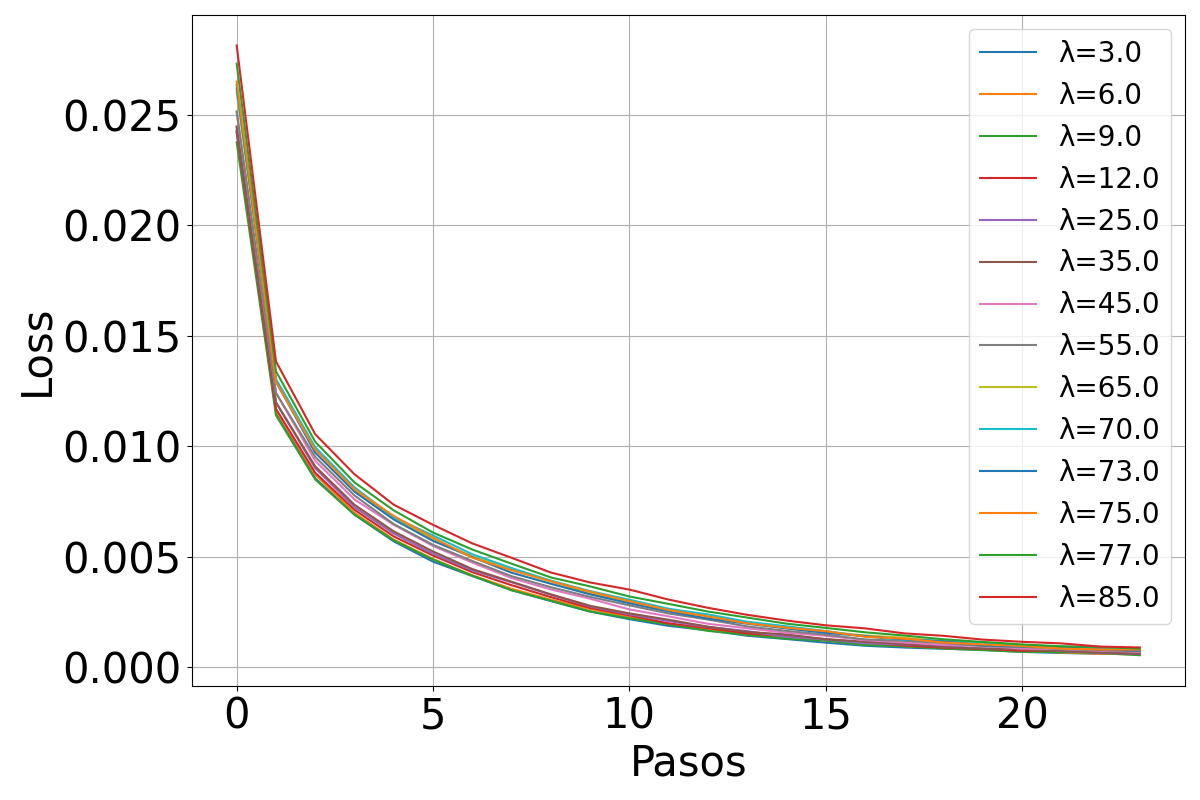
\includegraphics[width=\linewidth]{images/Train_Loss_evolucion_fxshield.png}
        \caption{FX-SHIELD - Train Loss}
    \end{subfigure}
    \hfill
    \begin{subfigure}[b]{0.3\textwidth}
        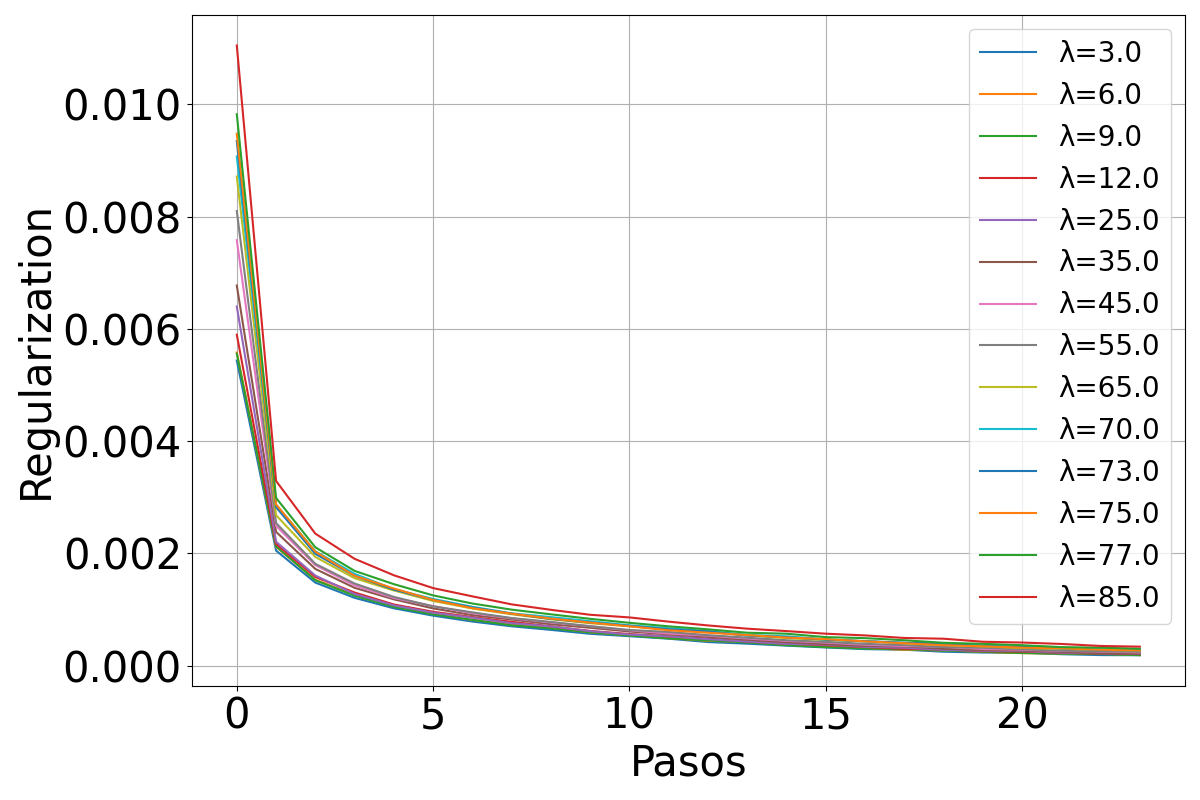
\includegraphics[width=\linewidth]{images/Train_Regularization_evolucion_fxshield.png}
        \caption{FX-SHIELD - Train Reg.}
    \end{subfigure}
    \hfill
    \begin{subfigure}[b]{0.3\textwidth}
        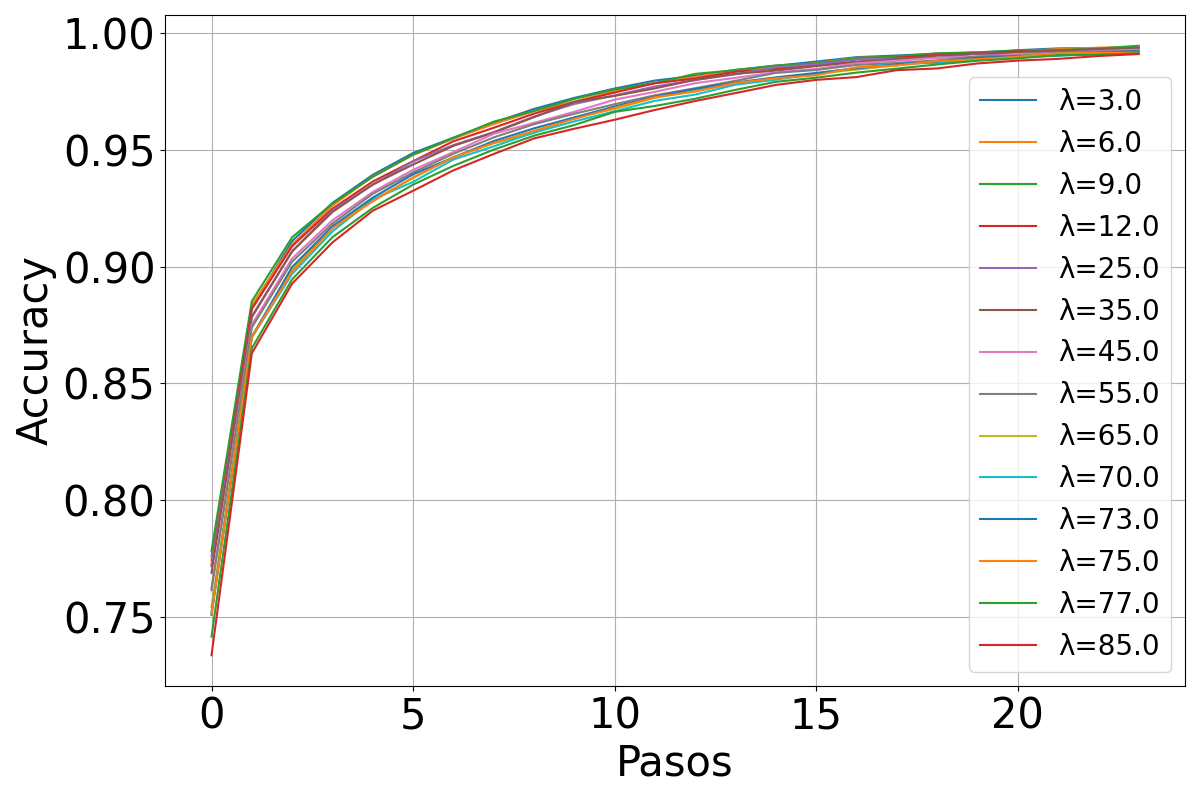
\includegraphics[width=\linewidth]{images/Train_Accuracy_evolucion_fxshield.png}
        \caption{FX-SHIELD - Train Acc.}
    \end{subfigure}

    \vspace{0.5em}

    % Fila 2: Val
    \begin{subfigure}[b]{0.3\textwidth}
        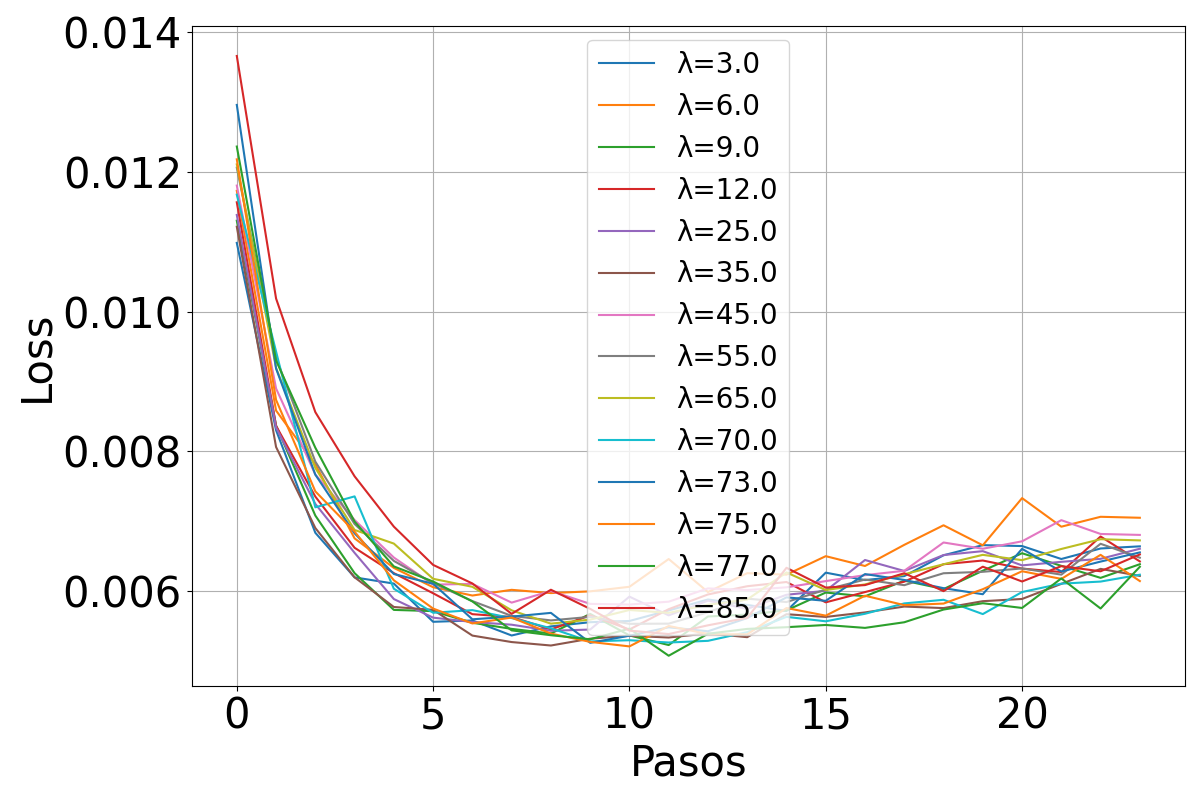
\includegraphics[width=\linewidth]{images/Val_Loss_evolucion_fxshield.png}
        \caption{FX-SHIELD - Val Loss}
    \end{subfigure}
    \hfill
    \begin{subfigure}[b]{0.3\textwidth}
        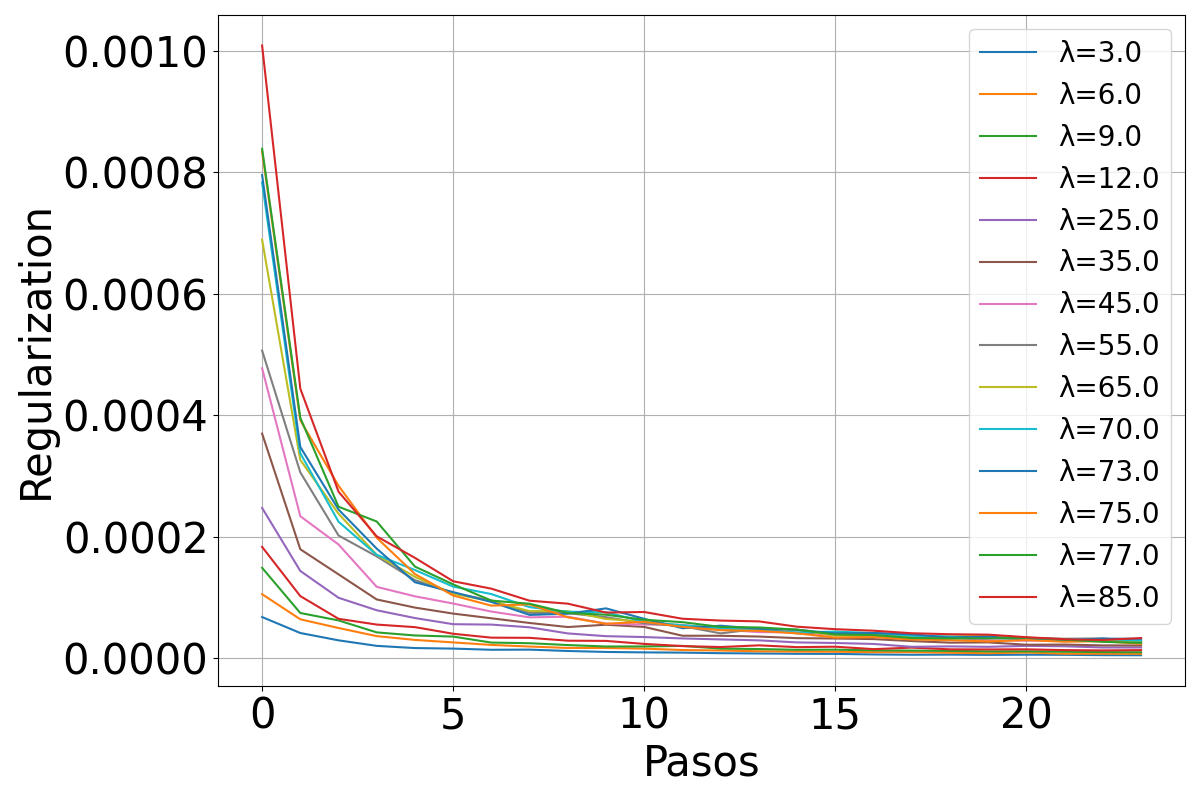
\includegraphics[width=\linewidth]{images/Val_Regularization_evolucion_fxshield.png}
        \caption{FX-SHIELD - Val Reg.}
    \end{subfigure}
    \hfill
    \begin{subfigure}[b]{0.3\textwidth}
        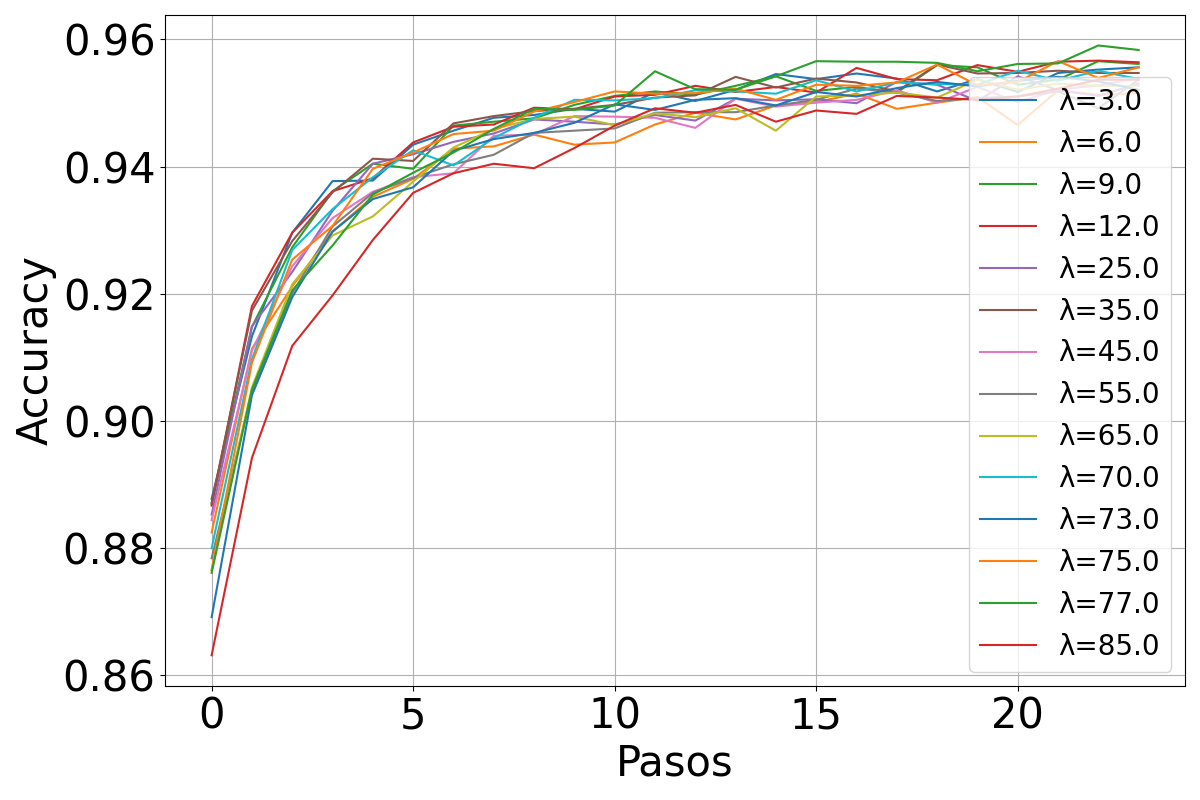
\includegraphics[width=\linewidth]{images/Val_Accuracy_evolucion_fxshield.png}
        \caption{FX-SHIELD - Val Acc.}
    \end{subfigure}

    \caption{Evolución de métricas para el modelo \texttt{FX-SHIELD}}
    \label{fig:metrics_fxshield}
\end{figure}

% === Figura: frshield ===
\begin{figure}[H]
    \centering
    % Fila 1: Train
    \begin{subfigure}[b]{0.3\textwidth}
        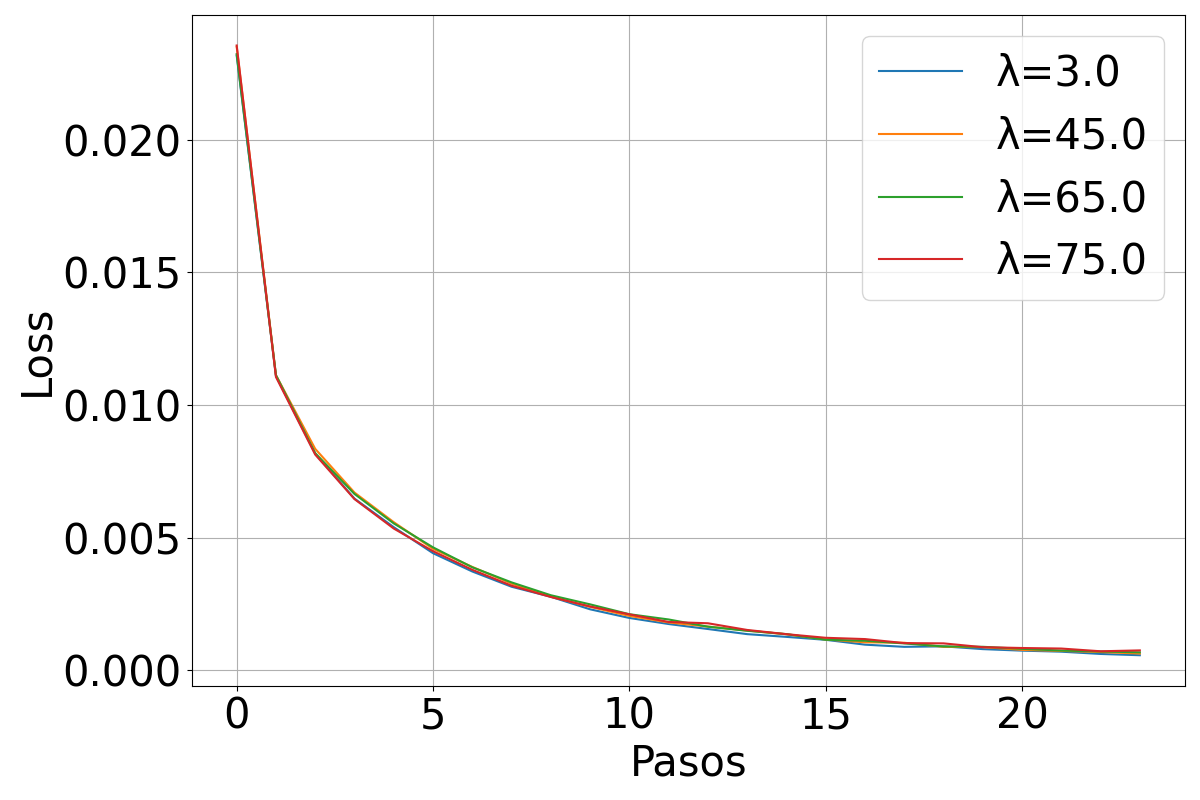
\includegraphics[width=\linewidth]{images/Train_Loss_evolucion_frshield.png}
        \caption{FRSHIELD - Train Loss}
    \end{subfigure}
    \hfill
    \begin{subfigure}[b]{0.3\textwidth}
        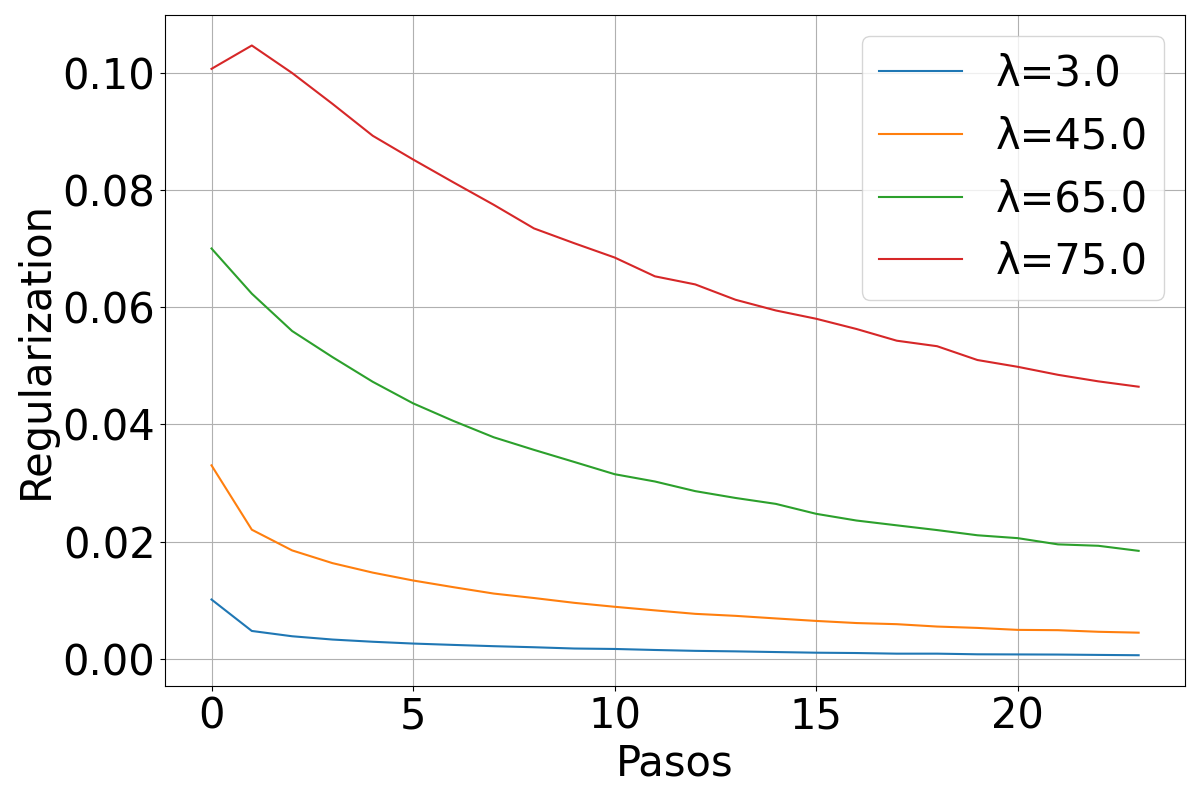
\includegraphics[width=\linewidth]{images/Train_Regularization_evolucion_frshield.png}
        \caption{FRSHIELD - Train Reg.}
    \end{subfigure}
    \hfill
    \begin{subfigure}[b]{0.3\textwidth}
        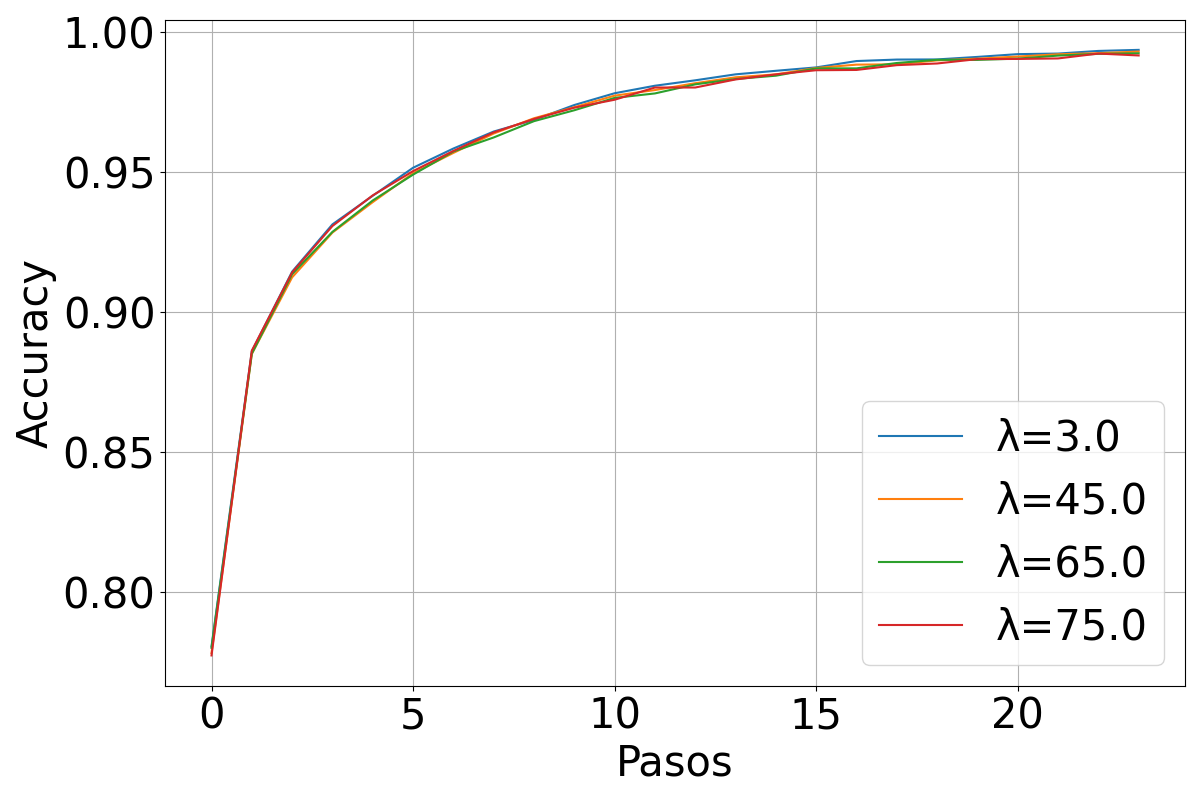
\includegraphics[width=\linewidth]{images/Train_Accuracy_evolucion_frshield.png}
        \caption{FRSHIELD - Train Acc.}
    \end{subfigure}

    \vspace{0.5em}

    % Fila 2: Val
    \begin{subfigure}[b]{0.3\textwidth}
        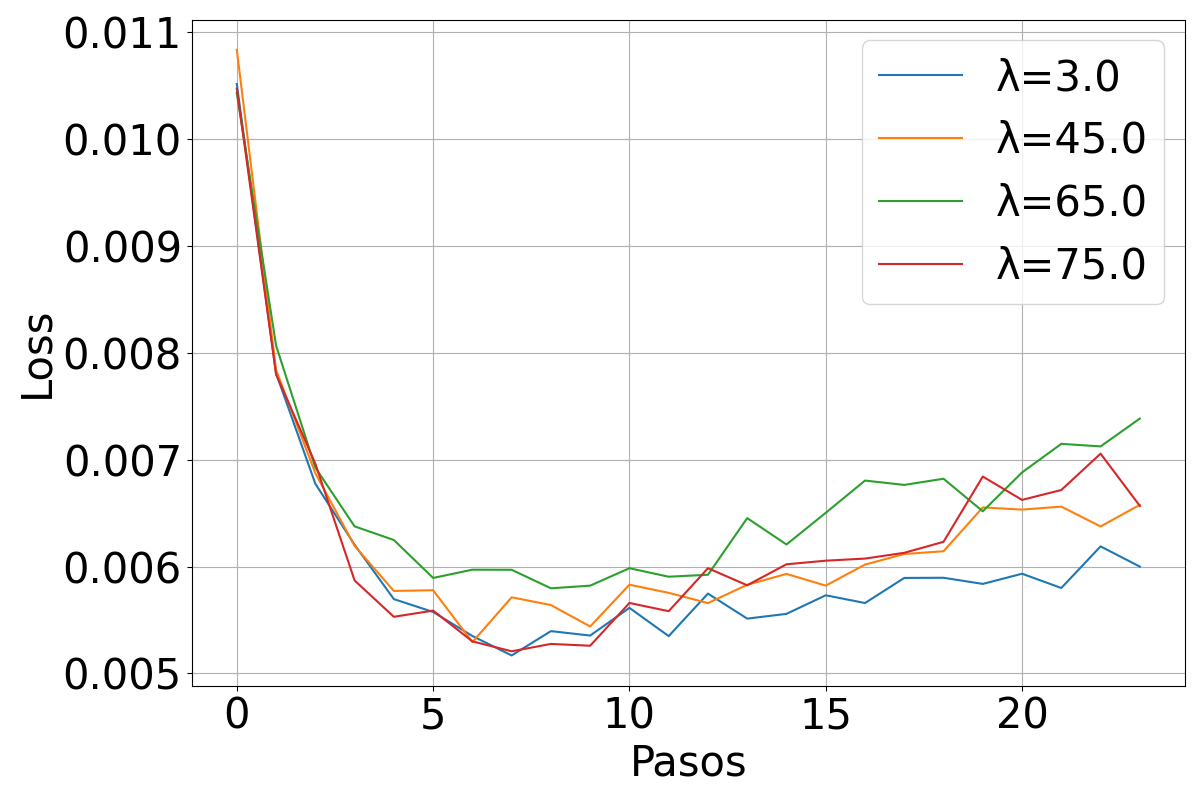
\includegraphics[width=\linewidth]{images/Val_Loss_evolucion_frshield.png}
        \caption{FRSHIELD - Val Loss}
    \end{subfigure}
    \hfill
    \begin{subfigure}[b]{0.3\textwidth}
        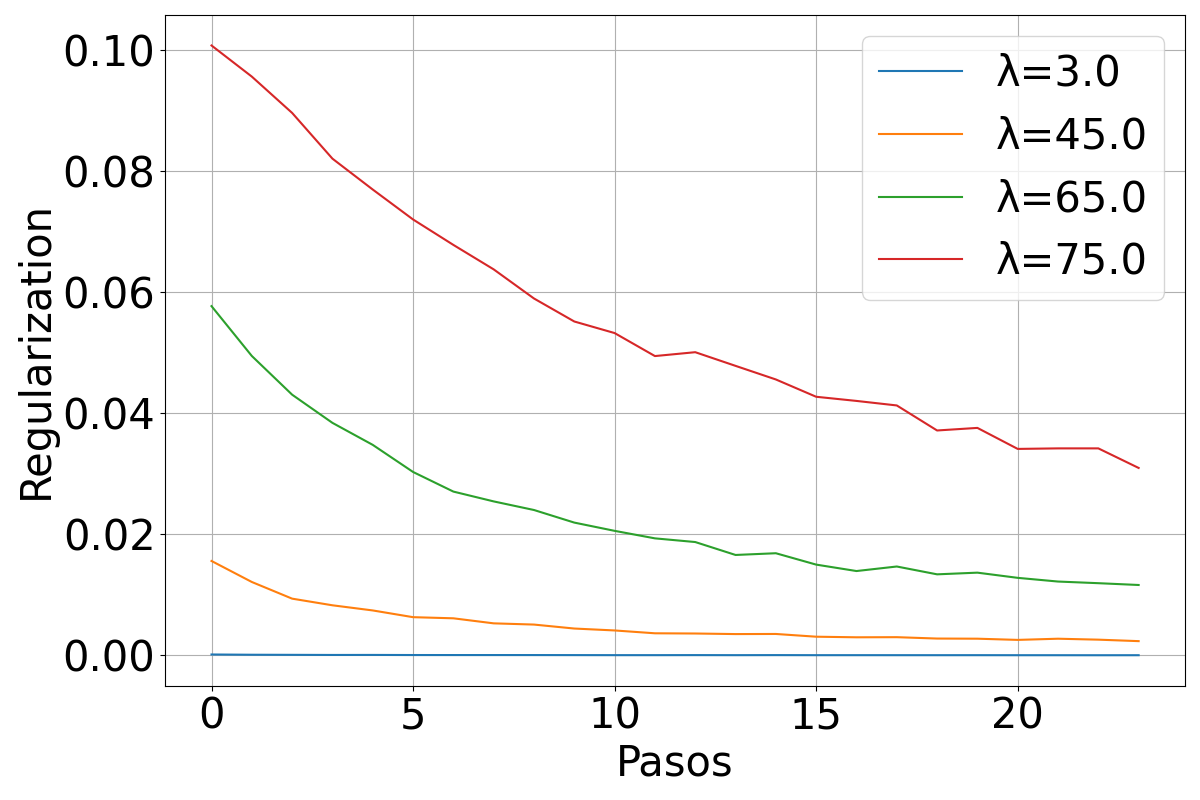
\includegraphics[width=\linewidth]{images/Val_Regularization_evolucion_frshield.png}
        \caption{FRSHIELD - Val Reg.}
    \end{subfigure}
    \hfill
    \begin{subfigure}[b]{0.3\textwidth}
        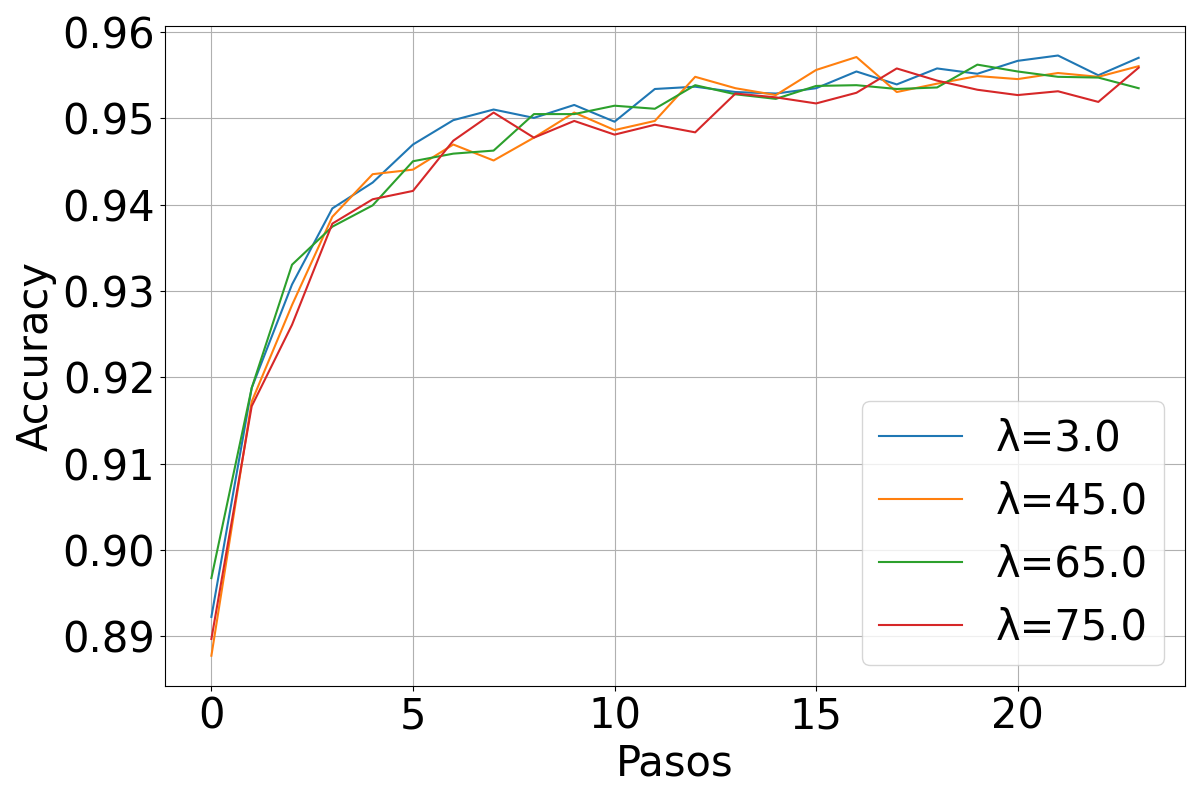
\includegraphics[width=\linewidth]{images/Val_Accuracy_evolucion_frshield.png}
        \caption{FRSHIELD - Val Acc.}
    \end{subfigure}

    \caption{Evolución de métricas para el modelo \texttt{FRSHIELD}}
    \label{fig:metrics_frshield}
\end{figure}

Finalmente para H-SHIELD (Figura \ref{fig:metrics_hshield}) se obtienen resultados parecidos a X-SHIELD. Observando su gráfica de pérdida en entrenamiento y en validación se que este método también podría beneficiarse de entrenar durante más épocas.

% === Figura: hshield ===
\begin{figure}[H]
    \centering
    % Fila 1: Train
    \begin{subfigure}[b]{0.3\textwidth}
        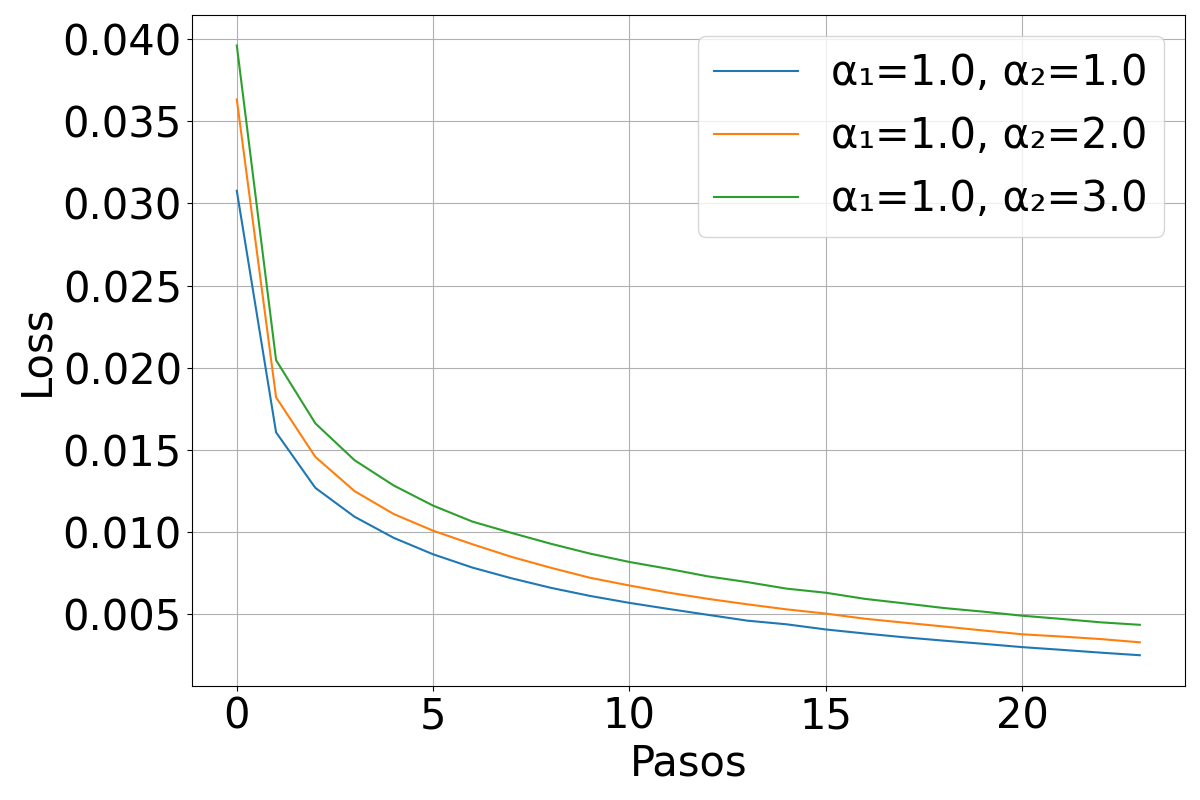
\includegraphics[width=\linewidth]{images/Train_Loss_evolucion_hshield.png}
        \caption{HSHIELD - Train Loss}
    \end{subfigure}
    \hfill
    \begin{subfigure}[b]{0.3\textwidth}
        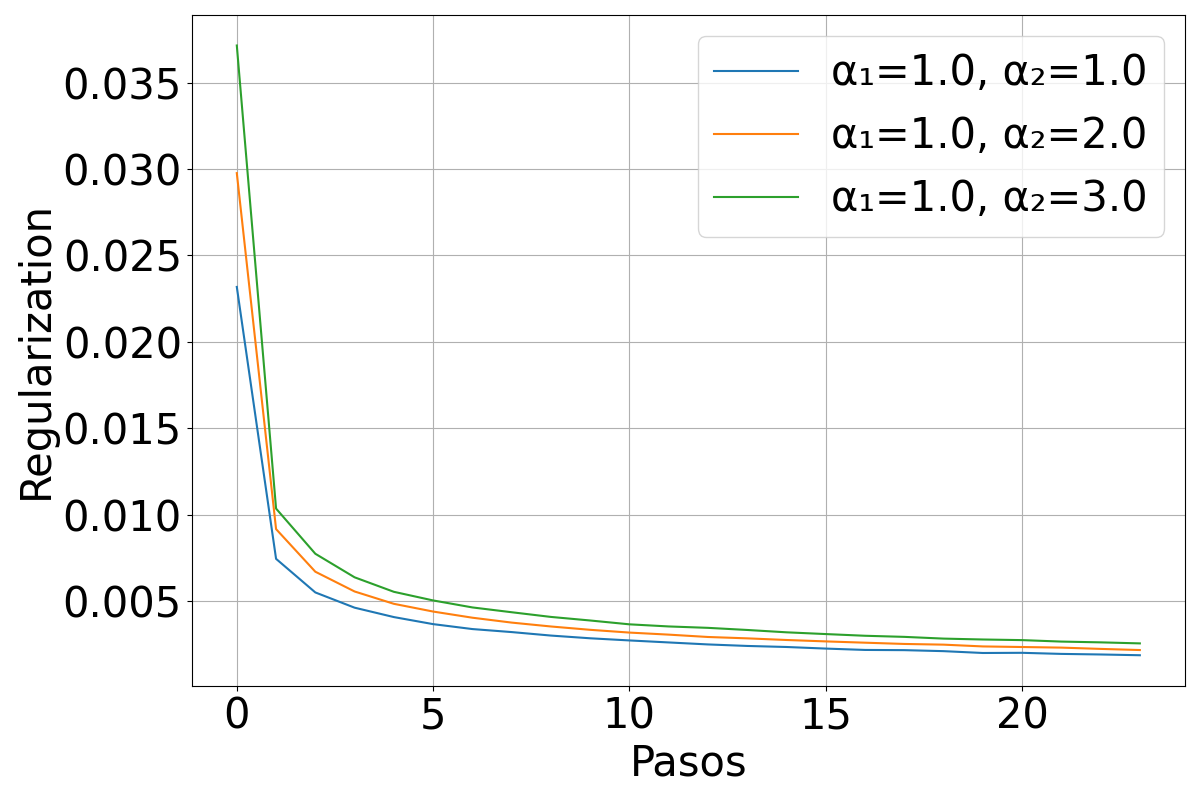
\includegraphics[width=\linewidth]{images/Train_Regularization_evolucion_hshield.png}
        \caption{HSHIELD - Train Reg.}
    \end{subfigure}
    \hfill
    \begin{subfigure}[b]{0.3\textwidth}
        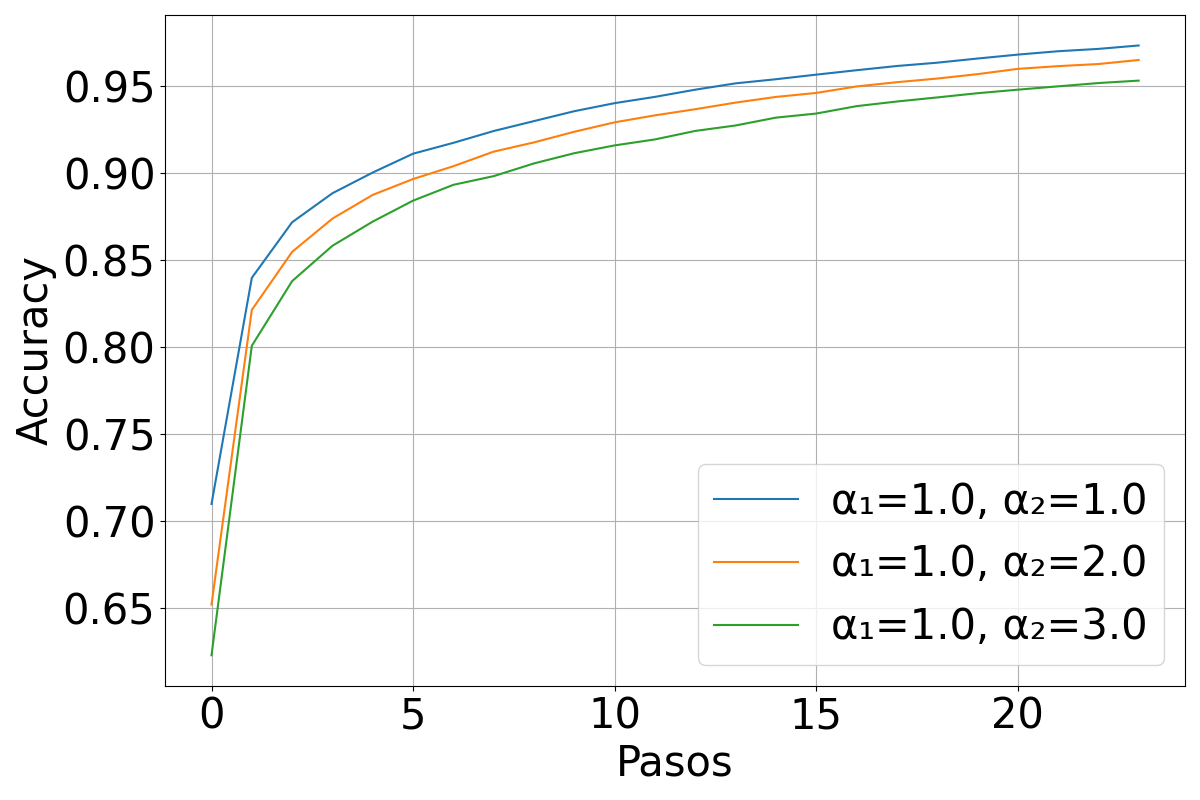
\includegraphics[width=\linewidth]{images/Train_Accuracy_evolucion_hshield.png}
        \caption{HSHIELD - Train Acc.}
    \end{subfigure}

    \vspace{0.5em}

    % Fila 2: Val
    \begin{subfigure}[b]{0.3\textwidth}
        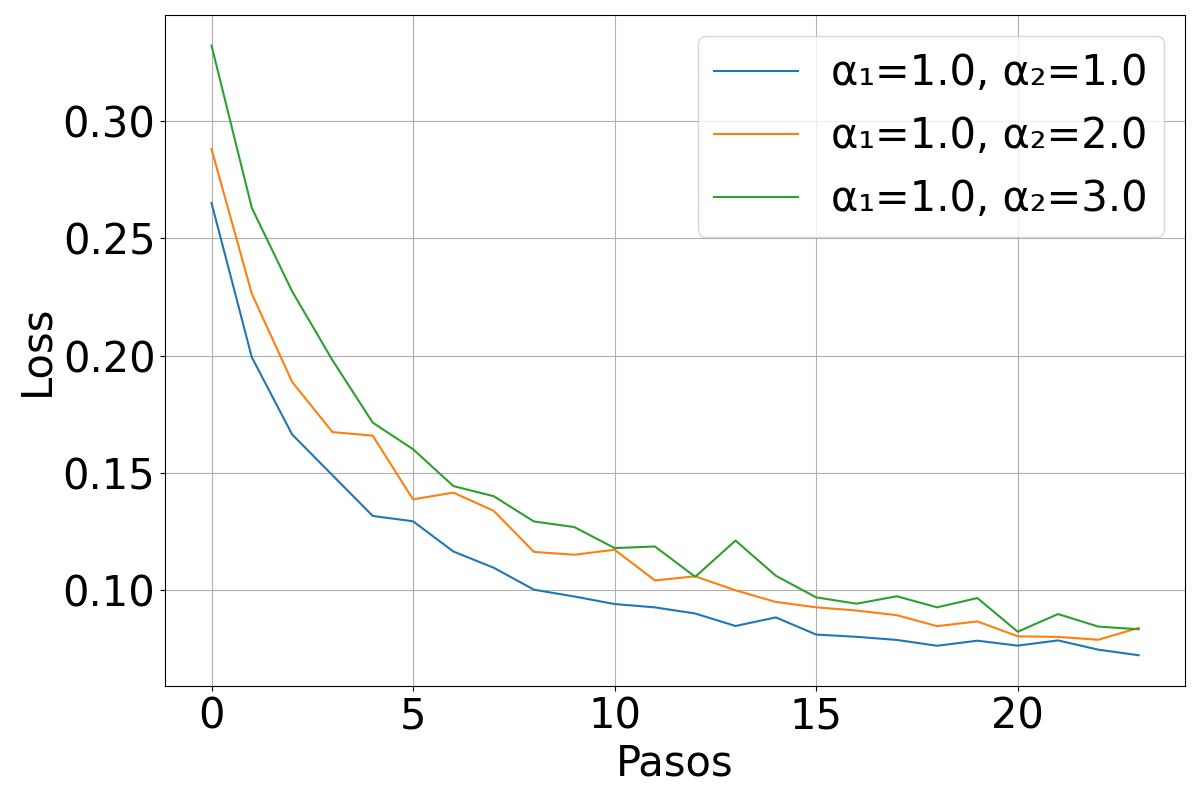
\includegraphics[width=\linewidth]{images/Val_Loss_evolucion_hshield.png}
        \caption{HSHIELD - Val Loss}
    \end{subfigure}
    \hfill
    \begin{subfigure}[b]{0.3\textwidth}
        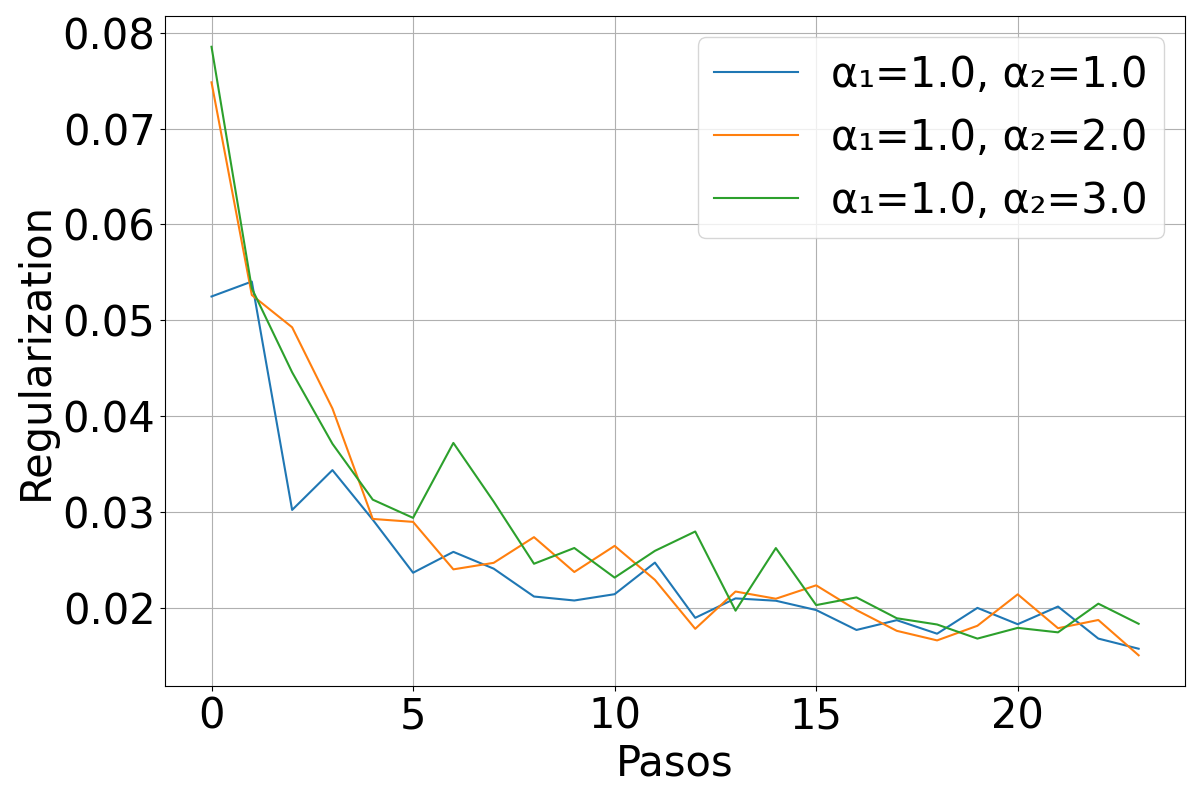
\includegraphics[width=\linewidth]{images/Val_Regularization_evolucion_hshield.png}
        \caption{HSHIELD - Val Reg.}
    \end{subfigure}
    \hfill
    \begin{subfigure}[b]{0.3\textwidth}
        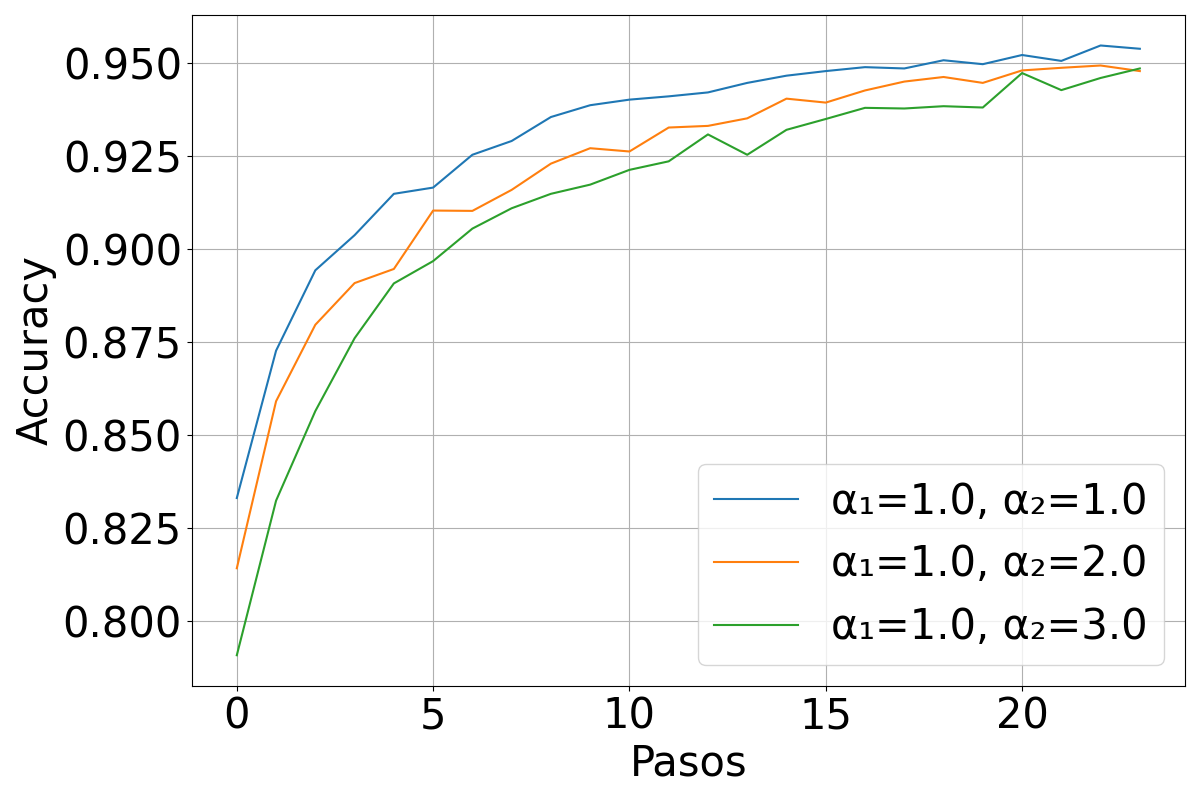
\includegraphics[width=\linewidth]{images/Val_Accuracy_evolucion_hshield.png}
        \caption{HSHIELD - Val Acc.}
    \end{subfigure}

    \caption{Evolución de métricas para el modelo \texttt{HSHIELD}}
    \label{fig:metrics_hshield}
\end{figure}

% === Figura: mejores modelos ===
%\begin{figure}[H]
%    \centering
%     Fila 1: Train
%    \begin{subfigure}[b]{0.3\textwidth}
%        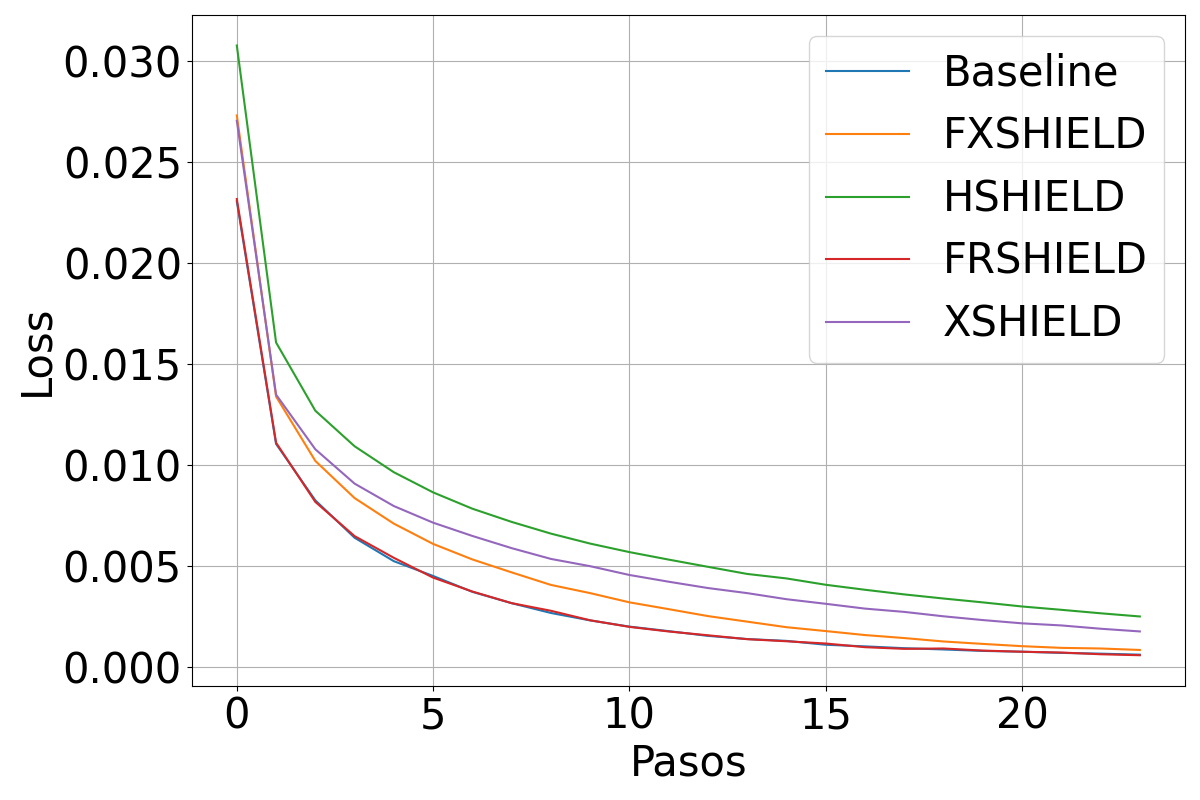
\includegraphics[width=\linewidth]{images/Train_Loss_comparacion.png}
%        \caption{Mejores modelos - Train Loss}
%    \end{subfigure}
%    \hfill
%    \begin{subfigure}[b]{0.3\textwidth}
%        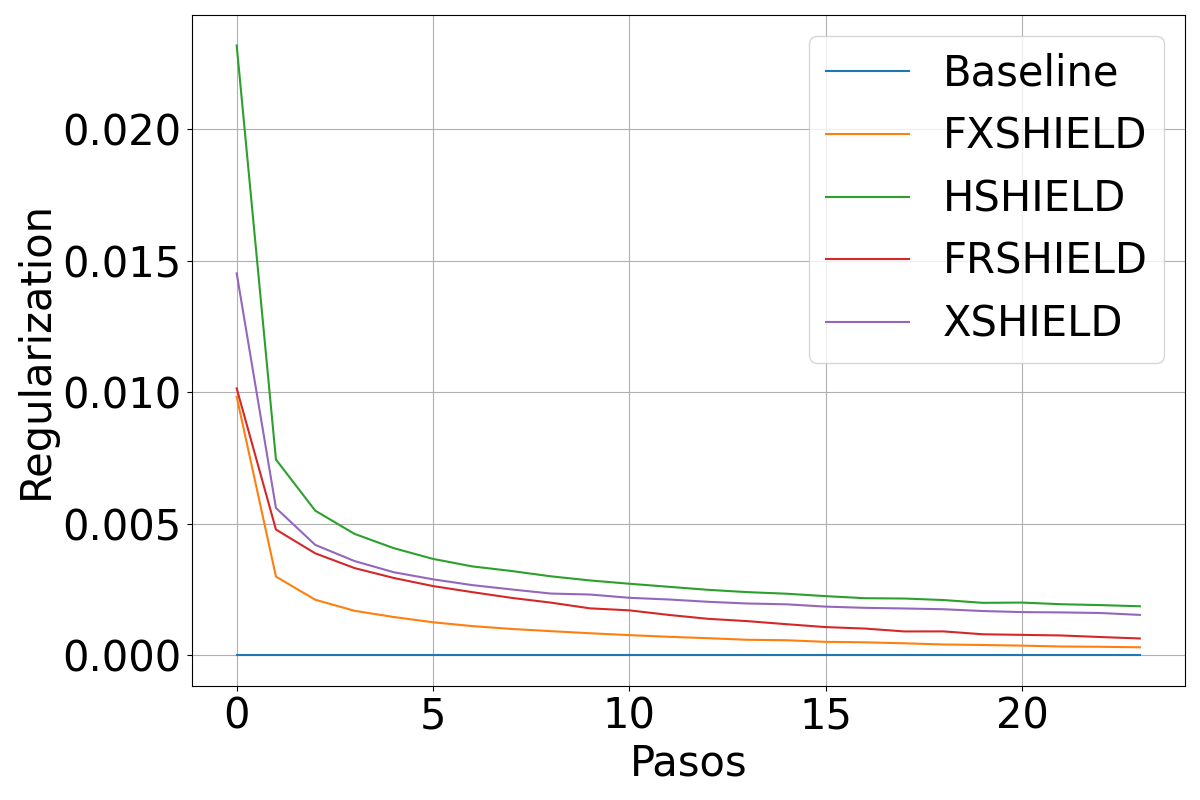
\includegraphics[width=\linewidth]{images/Train_Regularization_comparacion.png}
%        \caption{Mejores modelos - Train Reg.}
%    \end{subfigure}
%    \hfill
%    \begin{subfigure}[b]{0.3\textwidth}
%        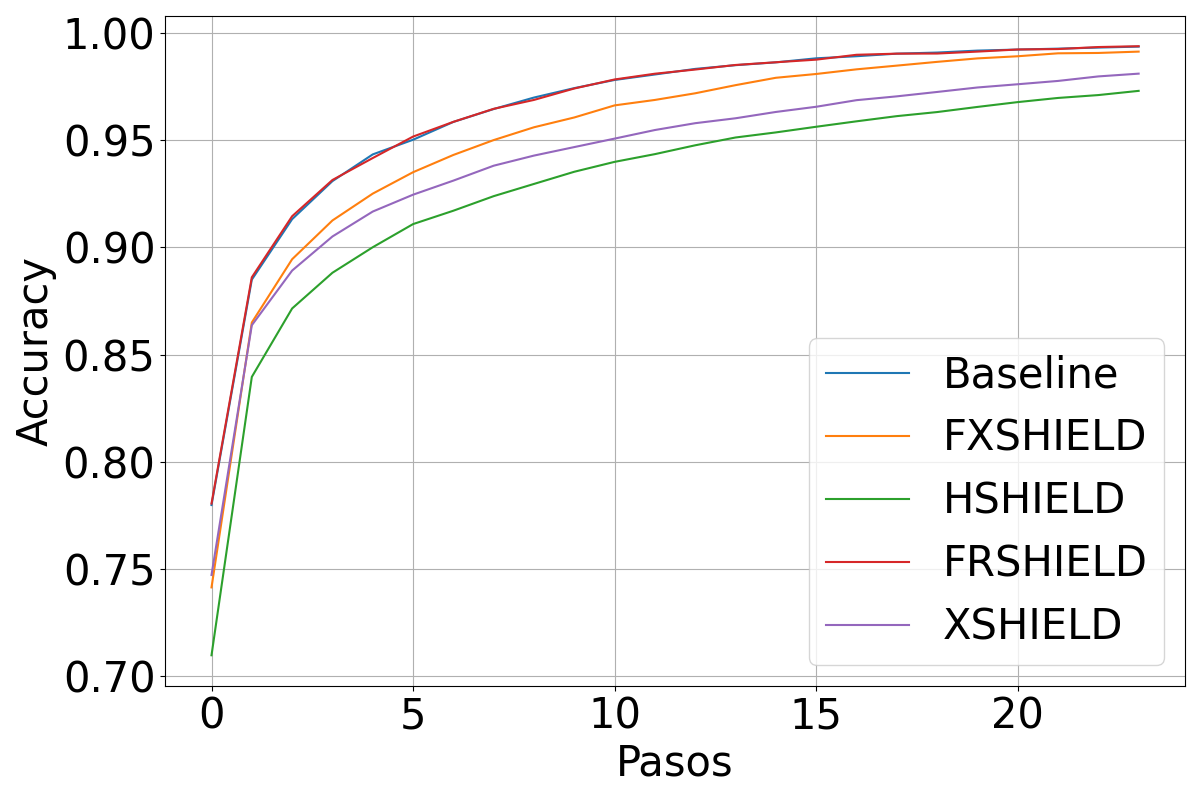
\includegraphics[width=\linewidth]{images/Train_Accuracy_comparacion.png}
%        \caption{Mejores modelos - Train Acc.}
%    \end{subfigure}
%
%    \vspace{0.5em}
%
%    % Fila 2: Val
%    \begin{subfigure}[b]{0.3\textwidth}
%        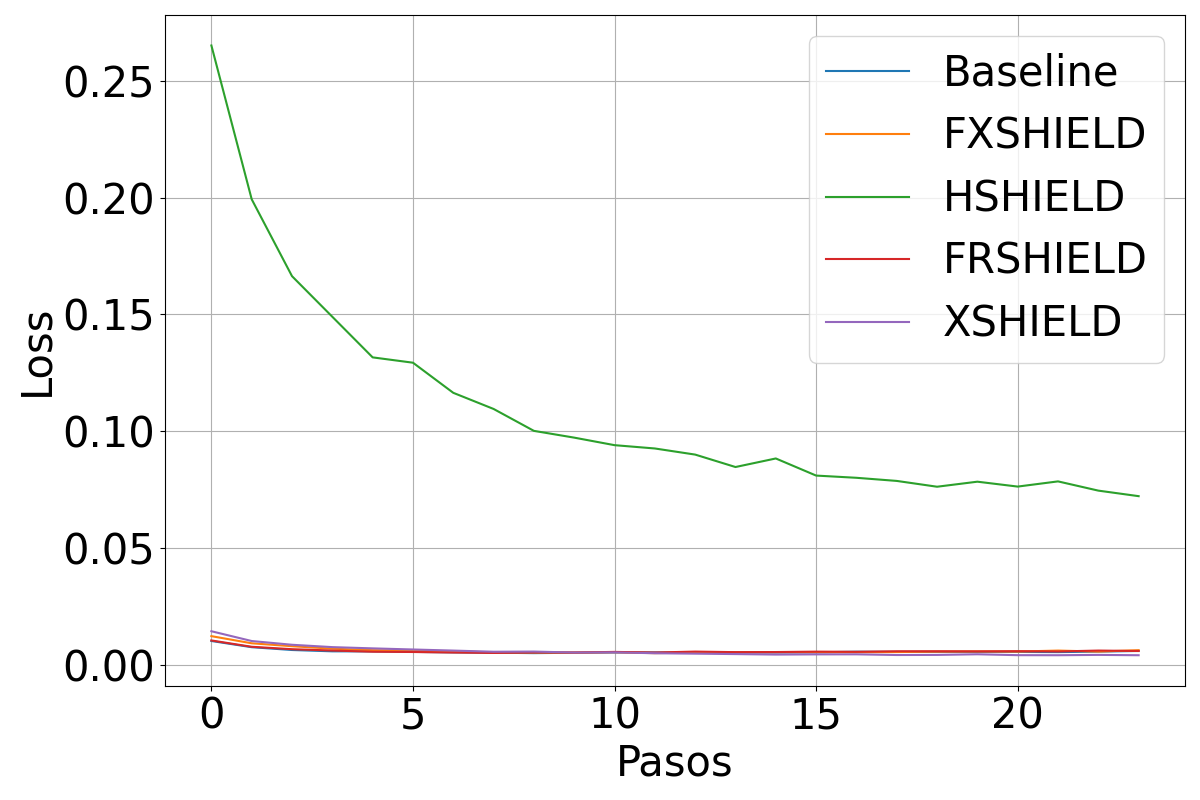
\includegraphics[width=\linewidth]{images/Val_Loss_comparacion.png}
%        \caption{Mejores modelos - Val Loss}
%    \end{subfigure}
%    \hfill
%    \begin{subfigure}[b]{0.3\textwidth}
%        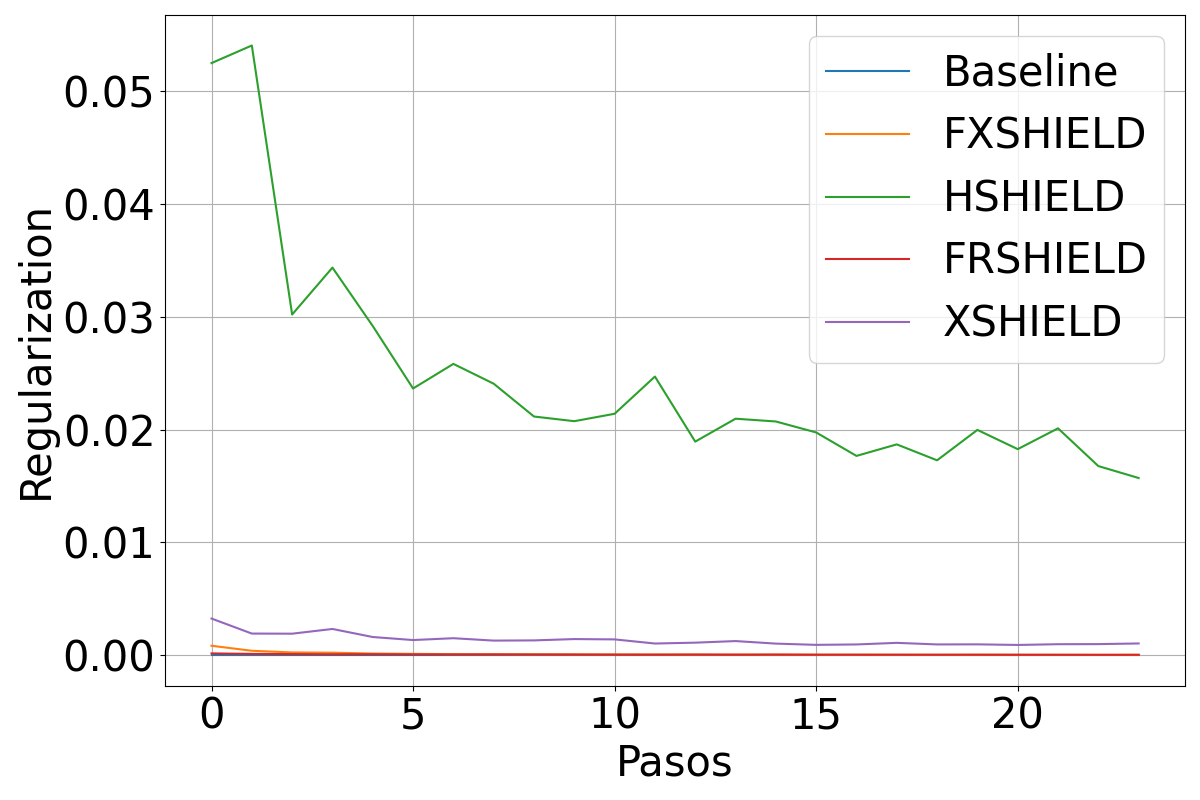
\includegraphics[width=\linewidth]{images/Val_Regularization_comparacion.png}
%        \caption{Mejores modelos - Val Reg.}
%    \end{subfigure}
%    \hfill
%    \begin{subfigure}[b]{0.3\textwidth}
%        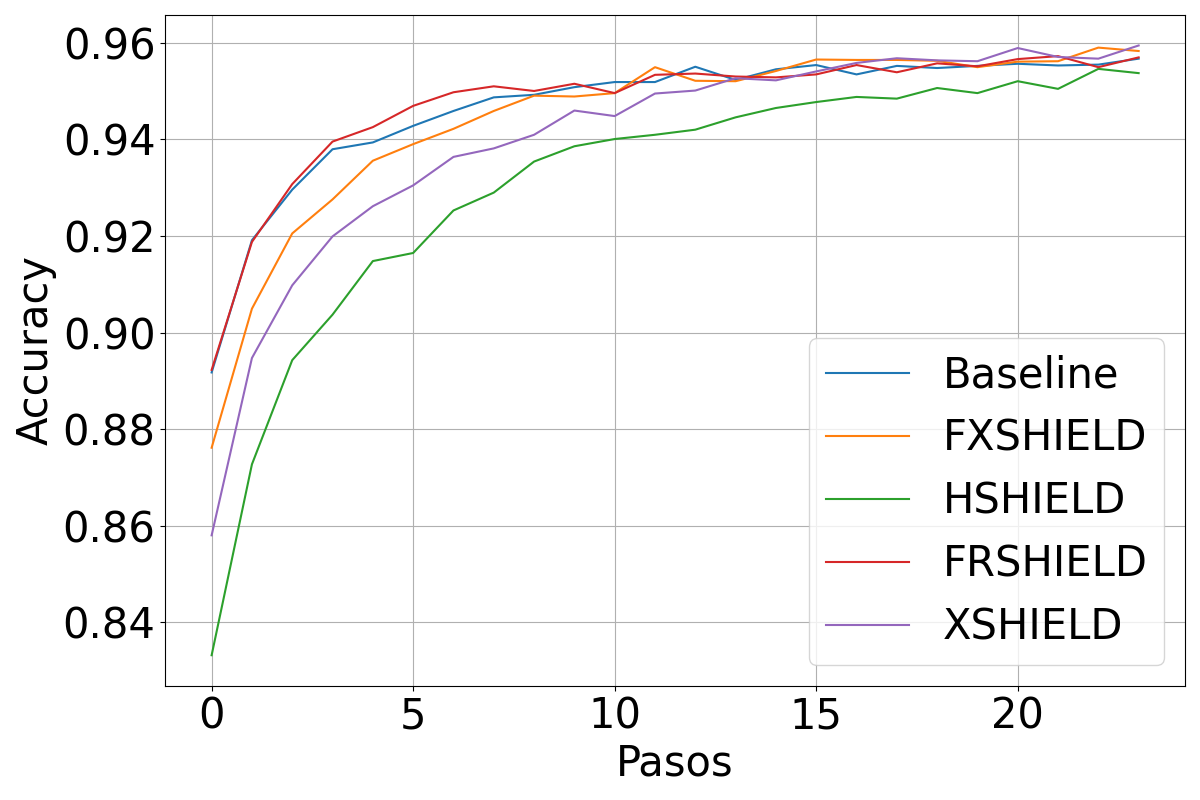
\includegraphics[width=\linewidth]{images/Val_Accuracy_comparacion.png}
%        \caption{Mejores modelos - Val Acc.}
%    \end{subfigure}
%
%    \caption{Evolución de métricas para los mejores modelos.}
%    \label{fig:metrics_mejores}
%\end{figure}

\subsection{Métricas REVEL}

Vemos en la Figura \ref{fig:violinplots} como se distribuyen las 100 medidas por métrica REVEL para cada método. Los métodos FX-SHIELD, X-SHIELD y H-SHIELD tienen distribuciones casi idénticas para la \textit{local concordance} y para la \textit{local fidelity}. Tienen distribuciones muy concentradas al valor máximo. Por otro lado FR-SHIELD tiene un distribución parecida pero menos concentrada, con mayor varianza. 

X-SHIELD y H-SHIELD tienen un distribución de la \textit{Robustness} parecida, con H-SHIELD un poco mayor. Para FX-SHIELD esta es claramente más baja. FR-SHIELD presenta la peor distribución de los cuatro métodos con mayor varianza.

De los \textit{violin plots} de la \textit{conciseness} no se puede discernir nada con una inspección visual excepto que la distribución para FR-SHIELD es muy distinta a la de los otros métodos.

Por último, para la \textit{prescriptivity} se tienen dos distribuciones parecidas para X-SHIELD y H-SHIELD, estando la de X-SHIELD desplazada hacia arriba. Por otro lado se tienen la de FX-SHIELD y FR-SHIELD que son parecidas también. A simple vista no es fácil ver cual de las dos podría ser mejor.


\begin{figure}[H]
    \centering
    
    \begin{subfigure}[b]{0.45\textwidth}
        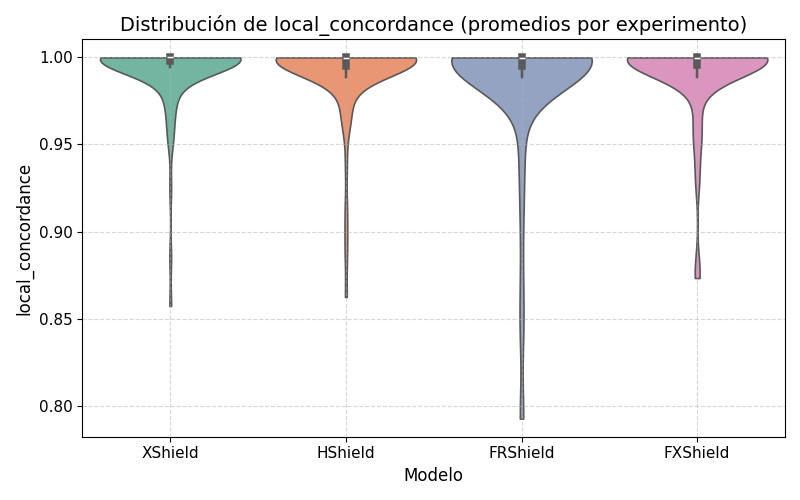
\includegraphics[width=\linewidth]{images/boxplot_local_concordance.png}
        \caption{Local Concordance}
    \end{subfigure}
    \hfill
    \begin{subfigure}[b]{0.45\textwidth}
        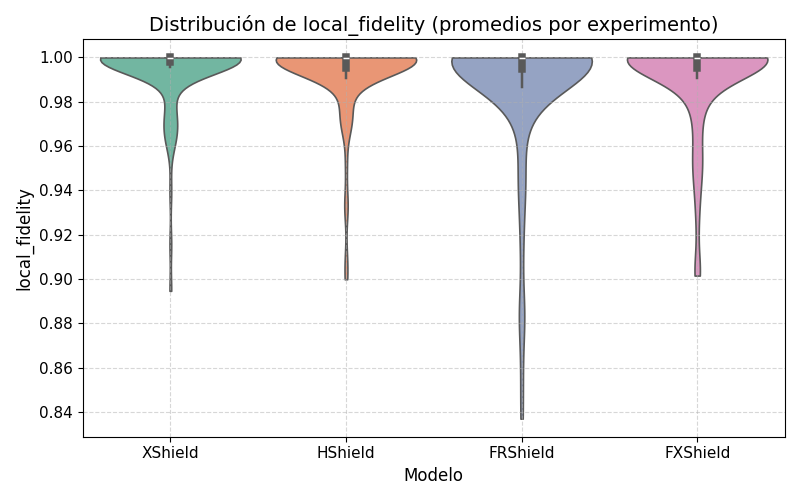
\includegraphics[width=\linewidth]{images/boxplot_local_fidelity.png}
        \caption{Local Fidelity}
    \end{subfigure}    
    
    \begin{subfigure}[b]{0.45\textwidth}
        \includegraphics[width=\linewidth]{images/boxplot_robustness.png}
        \caption{Robustness}
    \end{subfigure}
    \hfill
    \begin{subfigure}[b]{0.45\textwidth}
        \includegraphics[width=\linewidth]{images/boxplot_conciseness.png}
        \caption{Conciseness}
    \end{subfigure}

    \begin{subfigure}[b]{0.45\textwidth}
        \includegraphics[width=\linewidth]{images/boxplot_prescriptivity.png}
        \caption{Prescriptivity}
    \end{subfigure}
    \hfill
    \begin{subfigure}[b]{0.45\textwidth}
        \vspace{0.01\textheight} % Espacio vacío para mantener la alineación
    \end{subfigure}

    \caption{\textit{Violin plots} para las métricas de evaluación de explicaciones REVEL obtenidas para los modelos entrenados con las regularizaciones X-SHIELD, FX-SHIELD, FR-SHIELD y H-SHIELD.}
    \label{fig:violinplots}
\end{figure}

Los últimos resultados obtenidos vienen de los test bayesianos que hemos realizado sobre estas métricas. En la Tabla \ref{tab:bay-X-FX} se tiene que para la \textit{local concordance} y la \textit{local fidelity} de ambos métodos (X-SHIELD y FX-SHIELD) son iguales. Además FX-SHIELD mejora la \textit{prescriptivity} y la \textit{conciseness}, aunque esta última sin una diferencia estadísticamente significativa. De la misma forma, X-SHIELD presenta una mejor \textit{robustness}.

Para las comparaciones entre FX-SHIELD y FR-SHIELD (Tabla \ref{tab:bay-FX-FR}) tenemos que una vez más la \textit{local concordance} y la \textit{local fidelity} de ambos métodos coinciden completamente. FX-SHIELD mejora la \textit{conciseness} y \textit{prescriptivity} de FR-SHIELD, aunque únicamente con diferencia estadísticamente significativa en la primera. Por último ambas coinciden en su rendimiento en \textit{robustness}.

El último test realizado es entre FX-SHIELD y H-SHIELD (Tabla \ref{tab:bay-FX-H}). Otra vez ocurre que para la \textit{local concordance} y la \textit{local fidelity} de ambos métodos son iguales. FX-SHIELD mejora la \textit{prescriptivity} y la \textit{conciseness}, aunque esta última sin una diferencia estadísticamente significativa (pero muy alta igualmente). H-SHIELD mejora en \textit{robustness} de manera significativa a FX-SHIELD.



\begin{table}[ht]
\centering
\begin{tabular}{lccc}
\toprule
\textbf{Métrica} & \textbf{P(XShield $>$ FXShield)} & \textbf{P($=$)} & \textbf{P(FXShield $>$ XShield)} \\
\midrule
Local Fidelity    & 0.00\%  & 100.00\% & 0.00\%  \\
Local Concordance & 0.00\%  & 100.00\% & 0.00\%  \\
Conciseness       & 29.34\% & 0.00\%  & 70.66\%  \\
Prescriptivity    & 1.23\%  & 0.00\%  & 98.77\%  \\
Robustness        & 68.33\% & 31.67\% & 0.00\% \\
\bottomrule
\end{tabular}
\caption{Resultados de los tests bayesianos entre XShield y FXShield.}
\label{tab:bay-X-FX}
\end{table}

\begin{table}[ht]
\centering
\begin{tabular}{lccc}
\toprule
\textbf{Métrica} & \textbf{P(FXShield $>$ FRShield)} & \textbf{P($=$)} & \textbf{P(FRShield $>$ FXShield)} \\
\midrule
Local Fidelity    & 0.00\%  & 100.00\% & 0.00\%  \\
Local Concordance & 0.00\%  & 100.00\% & 0.00\%  \\
Conciseness       & 98.31\% & 0.00\%  & 1.69\%  \\
Prescriptivity    & 77.69\% & 0.00\%  & 22.31\%  \\
Robustness        & 12.28\% & 87.72\% & 0.00\% \\
\bottomrule
\end{tabular}
\caption{Resultados de los tests bayesianos entre FXShield y FRShield.}
\label{tab:bay-FX-FR}
\end{table}


\begin{table}[ht]
\centering
\begin{tabular}{lccc}
\toprule
\textbf{Métrica} & \textbf{P(FXShield $>$ HShield)} & \textbf{P($=$)} & \textbf{P(HShield $>$ FXShield)} \\
\midrule
Local Fidelity    & 0.00\%  & 100.00\% & 0.00\%  \\
Local Concordance & 0.00\%  & 100.00\% & 0.00\%  \\
Conciseness       & 83.28\% & 0.00\%  & 16.72\%  \\
Prescriptivity    & 99.99\% & 0.00\%  & 0.01\%  \\
Robustness        & 0.00\% & 1.29\% & 98.71\% \\
\bottomrule
\end{tabular}
\caption{Resultados de los tests bayesianos entre FXShield y HShield.}
\label{tab:bay-FX-H}
\end{table}


\section{Discusión} \label{sec:discusion}

Respecto al entrenamiento de los modelos el punto principal es que tanto X-SHIELD como H-SHIELD se podrían beneficiar de un mayor número de épocas.

Por otro lado hemos visto que X-SHIELD y H-SHIELD son regularizaciones centradas en mejorar la interpretabilidad del modelo que además consiguen una mejora en el rendimiento en clasificación. Sin embargo los métodos FX-SHIELD y FR-SHIELD mantienen prácticamente intacto este aspecto del modelo, aunque esto de por sí se puede considerar un aspecto positivo de estos ya que muchos métodos utilizados en XAI empeoran tienen un coste en el rendimiento a cambio de mejora de la interpretabilidad.

En cuanto a las métricas de interpretabilidad, recordemos el significado de estas. La \textit{local concordance} y la \textit{local fidelity} miden la similitud de la explicación al modelo de caja negra en el ejemplo y en su vecindario, respectivamente. Estas métricas deben ser muy cercanas a 1 para que la explicación se pueda considerar aceptable. Observemos en la Figura \ref{fig:violinplots} que este es el caso para todos nuestros métodos, y además en los tests bayesianos todos son equivalentes luego esto garantiza que nuestras explicaciones tengan un nivel bueno.

Por otro lado la \textit{prescriptivity} media si la explicación podía predecir correctamente los cambios necesarios en el ejemplo que hacen que cambie de clase. En este caso, nuestro método propuesto FX-SHIELD mejora de forma estadísticamente significativa al método X-SHIELD (también a H-SHIELD) y mejora de manera no significativa a FR-SHIELD. 

\textit{Conciseness} mide cómo de breves son las explicaciones. En esta métrica, una vez más FX-SHIELD es el ganador. Mejorando de manera significativa a FR-SHIELD y de manera no significativa a FX-SHIELD y H-SHIELD (aunque con probabilidad mayor al $70\%$ a ambas). Esto indica que las explicaciones producidas con FX-SHIELD son más fáciles de interpretar.

Cómo última métrica \textit{robustness} nos dice cómo de robusto es el modelo, en el sentido de cuanto varían las explicaciones generadas para el modelo de caja negra. En este caso X-SHIELD y H-SHIELD se presentan como las mejores opciones sobre FX-SHIELD. A su vez FR-SHIELD tiene tiene un rendimiento equivalente a FX-SHIELD en este sentido. 

En resumen el método propuesto FX-SHIELD es una versión mejor de FR-SHIELD (otro método propuesto) lo cual era de esperar porque FR-SHIELD es una versión aleatoria (menos informada) que FX-SHIELD. Por otro lado FX-SHIELD produce explicaciones más interpretables que X-SHIELD, aunque menos robustas. Por otro lado X-SHIELD mejora el rendimiento del modelo en la tarea de clasificación, mejorando la \textit{accuracy} en test. Nuestro último método propuesto H-SHIELD, que combina los métodos X-SHIELD y FX-SHIELD consigue capturar las ventajas de X-SHIELD (mejor \textit{accurcy} y mayor \textit{robustness}) pero no es capaz de mejorar a FX-SHIELD en el resto de métricas REVEL, sin embargo, es capaz de mejorar la robustez de las explicaciones respecto al método X-SHIELD. Además todos los métodos con los que hemos experimentado aseguran un mínimo de calidad en sus explicaciones al tener las métricas de \textit{local fidelity} y \textit{local concordance} prácticamente perfecta, con distribuciones muy concentradas alrededor del máximo.

\clearpage
\chapter{Conclusiones} \label{cap:conc}
Conclusiones del TFM y si he conseguido los objetivos que me propuse al inicio.

\section{Trabajos futuros}

Aquí comento trabajos futuros. Cómo probar con otros datsets o lo que comentamos de sacar las métricas REVEL sobre features (en nuestra primera charla).




% -------------------------------------------------------------------
% APPENDIX: Opcional
% -------------------------------------------------------------------

\appendix % Reinicia la numeración de los capítulos y usa letras para numerarlos
\pdfbookmark[-1]{Apéndices}{appendix} % Alternativamente podemos agrupar los apéndices con un nuevo \part{Apéndices}

%\begin{appendices}
\appendix
\chapter{Tablas de resultados} \label{APENDICEA}

En este apéndice se encuentran las tablas con las métricas  divididas por landmark para cada modelo propuesto y para el método geométrico original.
\begin{table}[h]
\noindent
\makebox[\textwidth]{\includegraphics[scale=0.9]{images/tabla_resultados_metodo_geometrico}}
\caption{Esta tabla contiene las métricas para el método geométrico introducido en \cite{GOMEZTRENADO2023106391} para nuestro conjunto test.}
\label{tab:tabla_resultados_metodo_geometrico}
\end{table}

\begin{table}[h]
\noindent
\makebox[\textwidth]{\includegraphics[scale=0.9]{images/tabla_resultados_clasificador}}
\caption{Esta tabla contiene las métricas para el modelo FSCNet con clasificador.}
\label{tab:tabla_resultados_clasificador}
\end{table}

\begin{table}[h]
\noindent
\makebox[\textwidth]{\includegraphics[scale=0.9]{images/tabla_resultados_clasificador_freeze}}
\caption{Esta tabla contiene las métricas para el modelo FSCNet con clasificador y los pesos de Resnet-18 congelados.}
\label{tab:tabla_resultados_clasificador_freeze}
\end{table}

\begin{table}[h]
\noindent
\makebox[\textwidth]{\includegraphics[scale=0.9]{images/tabla_resultados_hibrido}}
\caption{Esta tabla contiene las métricas para el modelo FSCNet híbrido.}
\label{tab:tabla_resultados_hibrido}
\end{table}

\begin{table}[h]
\noindent
\makebox[\textwidth]{\includegraphics[scale=0.9]{images/tabla_resultados_caracompleta}}
\caption{Esta tabla contiene las métricas para el modelo FSCNet con la cara completa.}
\label{tab:tabla_resultados_caracompleta}
\end{table}

\begin{table}[h]
\noindent
\makebox[\textwidth]{\includegraphics[scale=0.9]{images/tabla_resultados_caracompleta_normales}}
\caption{Esta tabla contiene las métricas para el modelo FSCNet con la cara completa y las normales de los landmarks1.}
\label{tab:tabla_resultados_caracompleta_normales}
\end{table}
\clearpage
\chapter{Curvas de aprendizaje} \label{APENDICEB}
En este apéndice se muestran las distintas curvas de aprendizaje obtenidas durante el entrenamiento de los modelos. Las curvas de aprendizaje muestran la evolución de la función de error en los conjuntos de entrenamiento y test a lo largo del proceso de entrenamiento. Mientras que hay un valor para el error en el conjunto de entrenamiento para cada iteración, el error en test se muestrea únicamente cada época completada. Además se ha añadido la gráfica de la evolución de la accuracy en entrenamiento también.

\begin{figure}[h]
\noindent
\makebox[\textwidth]{\includegraphics[scale=0.9]{images/curvas_clasificador}}
\caption{Curvas de aprendizaje para el modelo FSCNet + clasificador.}
\label{fig:curvas_clasificador}
\end{figure}

\begin{figure}[h]
\noindent
\makebox[\textwidth]{\includegraphics[scale=0.9]{images/curvas_clasificador_freeze}}
\caption{Curvas de aprendizaje para el modelo FSCNet + clasificador con los pesos de Resnet-18 congelados.}
\label{fig:curvas_clasificador_freeze}
\end{figure}

\begin{figure}[h]
\noindent
\makebox[\textwidth]{\includegraphics[scale=0.9]{images/curvas_hibrido}}
\caption{Curvas de aprendizaje para el modelo FSCNet híbrido.}
\label{fig:curvas_hibrido}
\end{figure}

\begin{figure}[h]
\noindent
\makebox[\textwidth]{\includegraphics[scale=0.9]{images/curvas_caracompleta}}
\caption{Curvas de aprendizaje para el modelo FSCNet con la cara completa.}
\label{fig:curvas_caracompleta}
\end{figure}

\begin{figure}[h]
\noindent
\makebox[\textwidth]{\includegraphics[scale=0.9]{images/curvas_caracompleta_normales}}
\caption{Curvas de aprendizaje para el modelo FSCNet con la cara completa + normales.}
\label{fig:curvas_caracompleta_normales}
\end{figure}

\clearpage
\chapter{Matrices de confusión} \label{APENDICEC}
En esta sección se muestran las distintas matrices de confusión obtenidas para los modelos presentados. Están divididas por landmarks.

\begin{figure}[h]
\noindent
\makebox[\textwidth]{\includegraphics[scale=0.7]{images/mc_geometrico}}
\caption{Matriz de confusión del método geométrico.}
\label{fig:mc_geometrico}
\end{figure}

\begin{figure}[h]
\noindent
\makebox[\textwidth]{\includegraphics[scale=0.7]{images/mc_clas}}
\caption{Matriz de confusión  de FSCNet con clasificador.}
\label{fig:mc_clas}
\end{figure}


\begin{figure}[h]
\noindent
\makebox[\textwidth]{\includegraphics[scale=0.7]{images/mc_clas_cong}}
\caption{Matriz de confusión de FSCNet con clasificador y pesos de Resnet-18 congelados.}
\label{fig:mc_clas_cong}
\end{figure}

\begin{figure}[h]
\noindent
\makebox[\textwidth]{\includegraphics[scale=0.7]{images/mc_hibrido}}
\caption{Matriz de confusión de FSCNet híbrido.}
\label{fig:mc_hibrido}
\end{figure}

\begin{figure}[h]
\noindent
\makebox[\textwidth]{\includegraphics[scale=0.7]{images/mc_cara}}
\caption{Matriz de confusión de FSCNet con cara completa .}
\label{fig:mc_cara}
\end{figure}

\begin{figure}[h]
\noindent
\makebox[\textwidth]{\includegraphics[scale=0.7]{images/mc_cara_normal}}
\caption{Matriz de confusión de FSCNet con cara completa + Normales.}
\label{fig:mc_cara_normal}
\end{figure}
\end{appendices}
% Añadir tantos apéndices como sea necesario 

% -------------------------------------------------------------------
% BACKMATTER
% -------------------------------------------------------------------

\backmatter % Desactiva la numeración de los capítulos
\pdfbookmark[-1]{Referencias}{BM-Referencias}

% BIBLIOGRAFÍA
%-------------------------------------------------------------------

\bibliographystyle{alpha-es} 
\begin{small} 
  \bibliography{biblio.bib}
\end{small}


\end{document}
